% ======================================================================
% Paper A of the meander series: the intuition paper and survey.
% Restructured 2026-10-25 from paper_expository_alpha/. New results are proved in papers B-D.
% Compile: tectonic main.tex
% ======================================================================
\documentclass[11pt]{article}
% Shared preamble for the meander paper series (papers A-D). Compile each paper with tectonic.
\usepackage[T1]{fontenc}
\usepackage[margin=1.15in]{geometry}
\usepackage{amsmath,amssymb,amsthm}
\usepackage{booktabs,array}
\usepackage{float}
\usepackage{tikz}
\usetikzlibrary{arrows.meta,decorations.pathmorphing,positioning}
\usepackage{pgfplots}
\pgfplotsset{compat=1.16}
\usepackage[colorlinks=true,linkcolor=blue!50!black,citecolor=blue!50!black,urlcolor=blue!50!black]{hyperref}

\newtheorem{theorem}{Theorem}
\newtheorem{proposition}[theorem]{Proposition}
\newtheorem{lemma}[theorem]{Lemma}
\newtheorem{corollary}[theorem]{Corollary}
\newtheorem{conjecture}[theorem]{Conjecture}
\theoremstyle{definition}
\newtheorem{definition}[theorem]{Definition}
\theoremstyle{remark}
\newtheorem*{remark}{Remark}

\emergencystretch=2em
\raggedbottom

% Tapes of the tape machine. Write -{}- for a double minus inside \tape{...} to avoid the
% typewriter dash ligature.
\newcommand{\tape}[1]{\texttt{#1}}
\newcommand{\hd}[1]{\texttt{[#1]}}

% Series line under the title.
\newcommand{\seriesline}[1]{\par\smallskip{\small\itshape Meander numbers: growth rate and exponent. #1}}

% The running example (order 3): upper arches (1,2), (3,6), (4,5); lower arches (1,6), (2,5), (3,4).
\newcommand{\meanderroad}{%
  \draw (1,0) arc[start angle=180,end angle=0,radius=0.5];
  \draw (3,0) arc[start angle=180,end angle=0,radius=1.5];
  \draw (4,0) arc[start angle=180,end angle=0,radius=0.5];
  \draw (1,0) arc[start angle=180,end angle=360,radius=2.5];
  \draw (2,0) arc[start angle=180,end angle=360,radius=1.5];
  \draw (3,0) arc[start angle=180,end angle=360,radius=0.5];
}
\newcommand{\meanderfigure}{%
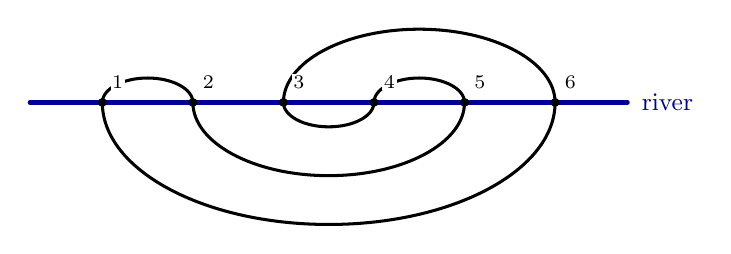
\begin{tikzpicture}[x=1.15cm,y=0.62cm,line cap=round]
  \draw[blue!60!black,line width=1.6pt] (0.2,0)--(6.8,0);
  \node[blue!60!black,anchor=west] at (6.85,0) {\small river};
  \begin{scope}[line width=1.1pt]\meanderroad\end{scope}
  \foreach \k in {1,...,6} {\fill (\k,0) circle[radius=1.6pt]; \node[fill=white,inner sep=0.6pt,font=\scriptsize] at (\k+0.17,0.42) {\k};}
\end{tikzpicture}}

% The series. Each paper cites the others as \cite{PaperA} etc.


% One tape drawn as a row of boxes: #1 shift, #2 comma list of + and -, #3 head index (as in Paper B).
\newcommand{\tp}[3]{%
  \begin{scope}[shift={#1}]
  \foreach \c [count=\i] in {#2} {
    \ifnum\i=#3\relax
      \draw[line width=0.9pt,fill=red!13] ({(\i-1)*0.36},-0.18) rectangle ++(0.36,0.36);
    \else
      \draw[line width=0.4pt] ({(\i-1)*0.36},-0.18) rectangle ++(0.36,0.36);
    \fi
    \node[font=\small,inner sep=0pt] at ({(\i-0.5)*0.36},0) {$\c$};
  }
  \end{scope}}

\title{Why $3.42$? The meander exponent,\\ from random walks to random surfaces\seriesline{Paper A.}}
\author{Carl Johan Ragnarsson}
\date{Draft of October 25, 2026}

\begin{document}
\maketitle

\begin{abstract}
A meander of order $n$ is a closed road that crosses a straight river $2n$ times without
crossing itself. The number $M_n$ of meanders of order $n$ is believed to grow like
$A\,\mu^n n^{-\alpha}$, with a constant $A$, $\mu\approx 12.26$ and
$\alpha=(29+\sqrt{145})/12\approx 3.4201$. The value of $\alpha$ comes from a physical argument
that treats a large meander as a random surface carrying two curves, and it has never been
proved. This paper, the first of a series of four, explains that argument from the beginning,
assuming no physics, and surveys what is now proved. The other papers contain the new results:
an exact encoding of meanders by walks on words and the bounds $12.2191\le\mu\le12.2970$
(Paper~B); the bounds $\mu^n e^{-C\sqrt n}\le M_n\le\mu^{n+1}/(8n)$ and an exactly solvable family
(Paper~C); and, in a continuum model of random surfaces, a proof that the analog of two spanning
trees has tail exponent $(17+\sqrt{145})/12$, which corresponds to the predicted
$\alpha_*=(29+\sqrt{145})/12$, together with a lower bound of the
predicted order in the conjectured limit of large meanders (Paper~D). Here we explain why these results hold and how they fit
together, and we describe the step that is still missing. All code was written using Claude
(Opus 5.5) or Codex (Sol 5.1) with active review and guidance throughout.
\end{abstract}

\tableofcontents

%%%%%%%%%%%%%%%%%%%%%%%%%%%%%%%%%%%%%%%%%%%%%%%%%%%%%%%%%%%%%%%%%%%%%%%%
\section{Introduction}\label{sec:intro}
%%%%%%%%%%%%%%%%%%%%%%%%%%%%%%%%%%%%%%%%%%%%%%%%%%%%%%%%%%%%%%%%%%%%%%%%

\subsection{The problem}

A \emph{meander of order $n$} is a closed road that crosses a straight river $2n$ times and
never crosses itself. Two drawings are the same meander if one can be deformed into the other
without changing the order of the crossings along the river. The number of meanders of order
$n$ is $M_n$:
\[ M_1, M_2, \ldots \;=\; 1,\ 2,\ 8,\ 42,\ 262,\ 1828,\ 13820,\ 110954,\ \ldots \]
Figure~\ref{fig:meander} shows one of the eight meanders of order $3$. Exact values have been
computed for every $n\le 32$~\cite{JG,JensenGit}; values for $33\le n\le 40$ have also been
computed privately, but they are not published or independently checked. No formula for $M_n$
is known.

\begin{figure}[t]
\centering
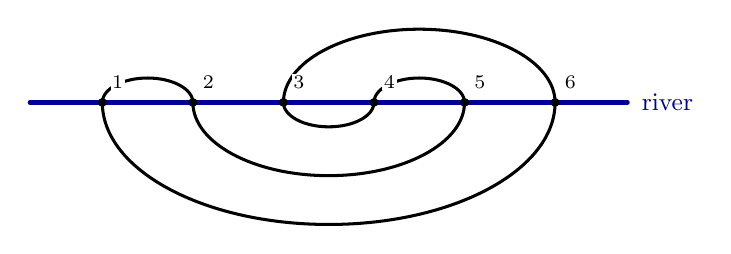
\begin{tikzpicture}[x=1.15cm,y=0.62cm,line cap=round]
  \draw[blue!60!black,line width=1.6pt] (0.2,0)--(6.8,0);
  \node[blue!60!black,anchor=west] at (6.85,0) {\small river};
  \begin{scope}[line width=1.1pt]\meanderroad\end{scope}
  \foreach \k in {1,...,6} {\fill (\k,0) circle[radius=1.6pt]; \node[fill=white,inner sep=0.6pt,font=\scriptsize] at (\k+0.17,0.42) {\k};}
\end{tikzpicture}
\caption{A meander of order $3$. Above the river the road joins crossings $1$--$2$, $3$--$6$
and $4$--$5$; below it joins $1$--$6$, $2$--$5$ and $3$--$4$. Following the road from
crossing $1$ visits $1,2,5,4,3,6$ and returns to $1$.}
\label{fig:meander}
\end{figure}

The numbers are believed to follow the law
\begin{equation}\label{eq:law}
M_n \;\approx\; A\,\mu^n\, n^{-\alpha}
\end{equation}
for constants $A$, $\mu$ and $\alpha$, in the sense that the ratio of the two sides should tend to
one as $n\to\infty$. The two main constants carry different information.

\begin{itemize}
\item The growth rate $\mu=\lim M_n^{1/n}$ exists. Intuitively, a meander offers about $\mu$
choices each time its order grows by one, that is, for each further pair of crossings.
Extrapolation from the exact counts gives $\mu\approx 12.2629$, and the best proved bounds are
$12.2191\le\mu\le12.2970$ (Paper~B; see Section~\ref{sec:tape}).
\item The exponent $\alpha$ is a slow correction on top of the exponential growth. It measures
how much of the naive count $\mu^n$ survives the global requirement that the road closes into a
single loop. Physicists predict~\cite{DGG} that $\alpha$ equals
\begin{equation}\label{eq:alpha}
\alpha_* \;=\; \frac{29+\sqrt{145}}{12} \;\approx\; 3.4201,
\end{equation}
and numerical fits to the exact counts are consistent with it to about three decimal places
(Section~\ref{sec:estimate}). This is not proved. Throughout,
$\alpha$ denotes the true exponent, whatever it is, and $\alpha_*$ the predicted number.
\end{itemize}

The growth rate depends on every detail of the definition, while the exponent is expected to be
\emph{universal}: it should not change if the rules are altered in small ways
(Section~\ref{sec:walks}). The predicted value is also irrational, which has a concrete
consequence. For the exponentially bounded integer coefficients considered here, a linear differential equation
with polynomial coefficients would impose rational local exponents through the theory of
$G$-functions~\cite{Andre}. In the power-law setting above, this forces $\alpha$ to be rational;
Paper~C gives the precise argument. So if $\alpha=\alpha_*$, the generating function
$\sum M_n x^n$, the power series whose coefficients are the counts, satisfies no such equation,
and the usual exact methods of enumeration cannot reach it.

\subsection{What is known, and the papers of this series}

Write $u_n=M_n/\mu^n$ for the factor left over once the exponential growth is removed. The
prediction says $u_n\approx A\,n^{-3.4201}$. Table~\ref{tab:window} lines up what is proved.

\begin{table}[h]
\centering
\begin{tabular}{lll}
\toprule
 & lower bound & upper bound \\
\midrule
growth rate $\mu$ & $12.2191$ (Paper~B) & $12.2970$ (Paper~B) \\
proved for meanders: $u_n$ & $u_n\ge e^{-C\sqrt n}$ (Paper~C) & $u_n\le \mu/(8n)$ (Paper~C) \\
predicted: $u_n$ & $u_n\approx A\,n^{-3.4201}$ & $u_n\approx A\,n^{-3.4201}$\\
near-splits in the limit & exponent $3.4201$ (Paper~D) & exponent $3.134$ (Paper~D)\\
\bottomrule
\end{tabular}
\caption{What is proved, and what is predicted. The first row bounds the growth rate; the best
numerical estimate is $12.2629$. The middle rows concern the leftover factor $u_n=M_n/\mu^n$; $C$
is a constant. The last row concerns
the probability of a near-split in the conjectured limit of large meanders: an approximate
version of a meander splitting into two halves at the middle of the river
(Section~\ref{sec:limit}). Its predicted exponent is $\alpha_*$, and an exponent closer to
$\alpha_*$ is better on either side.}
\label{tab:window}
\end{table}

This paper is the first of four. It explains the intuition and surveys the results; the other
three contain the new results with their proofs. Here and below, a factor $n^{o(1)}$ is one that
grows more slowly than every positive power of $n$ and decays more slowly than every negative
power.
\begin{itemize}
\item \textbf{Paper~B}~\cite{PaperB}: \emph{the tape machine and bounds on the growth rate.} A
meander is encoded exactly by a walk on words in two letters that returns to its start
(Section~\ref{sec:tape}). Positive weights on these words give the upper bound, and a random rule
for choosing the steps of the walk gives the lower bound; together,
$12.2191\le\mu\le12.2970$, certified by exact computer checks.
\item \textbf{Paper~C}~\cite{PaperC}: \emph{the subexponential factor.} For meanders themselves,
as opposed to continuum models, $\mu^n e^{-C\sqrt n}\le M_n\le \mu^{n+1}/(8n)$
(Section~\ref{sec:proved}). Both bounds are new as far as we know; the lower bound improves one
obtained earlier in this project, which had an extra factor $\log n$ in the exponent. Paper~C also
contains an exactly solvable family of meanders with an irrational exponent
(Section~\ref{sec:band}), and precise statements of what would improve the bounds.
\item \textbf{Paper~D}~\cite{PaperD}: \emph{continuum results.} Ang, Park, Pfeffer and Sheffield
introduced a continuum model of random surfaces in which a surface is built from small squares
and its size is the number of squares. The continuum analog of the number of spanning trees (sets
of edges that reach every vertex without forming a loop) is a determinant. They proved that, among
surfaces with a given number of squares, weighting each surface by a power of this determinant
changes the model's single parameter by an exact amount. Paper~D supplies the normalization that
compares surfaces of different sizes, and proves how the probability that the surface has at least
$n$ squares decays with $n$. Together these show that, in this model, when surfaces are weighted
by the analog of two spanning trees, the total weight of surfaces with at least $n$ squares decays
like $n^{-x_2+o(1)}$, with $x_2=(17+\sqrt{145})/12$. This tail exponent corresponds to the
counting exponent $1+x_2=\alpha_*$ (Section~\ref{sec:continuum}).

Paper~D also studies the random surface that Borga, Gwynne and Sun conjecture to describe large
meanders (Section~\ref{sec:limit}). A meander of order $2m$ has a \emph{thin neck at the middle}
if the road crosses a vertical line through the middle of the river only twice; cutting along
the line then splits it into two meanders of order $m$. A \emph{near-split} is the continuum
version of such a neck, allowed to be imperfect by a fraction $\delta$ of the surface. Paper~D
proves that its probability is at least a constant times $\delta^{\alpha_*}$, the predicted
order, and at most a constant times $\delta^{3.134}$. Finally, Paper~D shows what a comparison
between finite meanders and the limit would give, for example
$M_n\ge\mu^n n^{-\alpha_*-o(1)}$ (Section~\ref{sec:bridge}).
\end{itemize}
Earlier exact formulas for related families are collected in~\cite{ExactPaper}.

\subsection{How the paper is organized}

The first half explains where~\eqref{eq:alpha} comes from. Section~\ref{sec:walks} shows the same
kind of exponent for random walks, where everything can be computed, and explains universality.
It then describes two ways to read a meander as a walk. Section~\ref{sec:surfaces} turns a
meander into a random surface with two curves drawn on it and explains the formula that produces
$3.4201$.

The second half surveys what is proved. Section~\ref{sec:proved} treats finite meanders.
Section~\ref{sec:continuum} describes the continuum model in which the KPZ formula, the rule
behind~\eqref{eq:alpha}, is a theorem.
Section~\ref{sec:limit} describes the conjectured limit of large meanders.
Section~\ref{sec:bridge} explains the missing step, from the continuum back to finite meanders,
by comparison with percolation (a classical model of random clusters on a lattice, where the
same step was carried out), and lists open problems.

\subsection{Status of the results}

The background in Sections~\ref{sec:walks} and~\ref{sec:surfaces} is either classical or a
physical prediction, and we say which. Except where noted, every result of the project quoted here
is new as far as we know, and each is proved in Paper~B, C or D, with a pointer to the complete proof in the project repository~\cite{Repo},
except one result on meandric systems in Section~\ref{sec:shape}, whose proof is only in the
repository. Most of these proofs were checked by at least one separate, independent reading; each
paper says which were not, and we repeat this where it matters. Nothing has been reviewed
outside the project. This paper gives short arguments where they explain something and
otherwise points to the paper that has the proof. Appendix~\ref{app:repo} says where in the
repository the proofs and data are.

%%%%%%%%%%%%%%%%%%%%%%%%%%%%%%%%%%%%%%%%%%%%%%%%%%%%%%%%%%%%%%%%%%%%%%%%
\section{Exponents of walks, and meanders as walks}\label{sec:walks}
%%%%%%%%%%%%%%%%%%%%%%%%%%%%%%%%%%%%%%%%%%%%%%%%%%%%%%%%%%%%%%%%%%%%%%%%

\subsection{Walks that come back}

Consider walks of $2n$ steps, each step up or down by one. There are $4^n$ of them. The number
that end where they started is
\[ \binom{2n}{n} \;\approx\; \frac{4^n}{\sqrt{\pi n}} . \]
The factor $n^{-1/2}$ has a simple meaning. After $2n$ steps a walk is typically at distance
about $\sqrt n$ from its start, spread over about $\sqrt n$ possible endpoints, so the chance of
landing exactly on the start is about $1/\sqrt n$.

Now ask in addition that the walk never goes below its starting level. By the ballot theorem,
exactly one in $n+1$ of the walks that come back has this property. The count is the Catalan
number
\begin{equation}\label{eq:catalan}
\mathrm{Cat}_n \;=\; \binom{2n}{n}\cdot\frac{1}{n+1} \;\approx\; \frac{4^n}{\sqrt\pi}\, n^{-1/2}\cdot n^{-1} .
\end{equation}
So the exponent $3/2$ adds up the costs of two global requirements: $1/2$ for coming back and
$1$ for staying above.

These walks are already part of a meander. The road above the river is a set of arches, each
joining two crossings, that do not cross each other; such a set is an \emph{arch system}.
Read the crossings from left to right and write an up step where an arch opens and a down step
where it closes: the result is a walk that comes back and never goes below its start, and every
such walk arises exactly once. So there are $\mathrm{Cat}_n$ choices above the river and
$\mathrm{Cat}_n$ below, and
\[ \mathrm{Cat}_n^2 \;\approx\; \frac{16^n}{\pi}\, n^{-3} \]
pairs of arch systems. A meander is a pair whose arches form a single loop. Requiring one loop
lowers the growth rate from $16$ to $\mu\approx 12.26$ and, by the prediction, raises the
exponent from $3$ to $3.42$.

\subsection{Universality}

Change the allowed steps: allow flat steps of length one as well, or long flat steps of length two. The number
of walks that come back without going below the start grows at a different rate, because there
are more choices per step. The exponent does not change. Table~\ref{tab:walks} reads it off the
exact counts.

\begin{table}[h]
\centering
\begin{tabular}{llcccc}
\toprule
requirement & steps & $\mu$ & $n=10$ & $n=100$ & $n=300$\\
\midrule
come back & up, down & $4$ & $0.4881$ & $0.4988$ & $0.4996$\\
come back, stay above & up, down & $4$ & $1.4010$ & $1.4889$ & $1.4963$\\
come back, stay above & up, down, flat & $3$ & $1.3019$ & $1.4762$ & $1.4919$\\
come back, stay above & up, down, long flat & $3+2\sqrt2$ & $1.3986$ & $1.4887$ & $1.4962$\\
\bottomrule
\end{tabular}
\caption{The exponent read off at size $n$ from exact counts $a_n$, by solving
$a_{n+1}/(\mu a_n)=(n/(n+1))^{\alpha}$ for $\alpha$. The limits are $1/2$ in the first row and
$3/2$ in the others. For the up-down walks and the walks with long flat steps (of length two),
$n$ is half the length; for the walks with flat steps of length one, $n$ is the length.}
\label{tab:walks}
\end{table}

The reason is that, zoomed out, all these walks look alike. A long walk with small steps,
rescaled so that its length is one and its typical height is one, looks like the same jagged
random curve, called Brownian motion, whatever the individual steps are~\cite{Donsker}. The growth rate
counts choices per step, so it depends on every detail. The exponent comes from the
probability of a global event, such as coming back or never going below the start, and that
probability can be computed in the zoomed-out picture, which is the same for all the walks.
Intuitively, $\mu$ is local and $\alpha$ is global.

A family of models with the same zoomed-out picture is called a \emph{universality class}. The
rule of thumb is that an exponent such as $\alpha$ depends only on what kind of object is being
counted, what is drawn on it, and which global conditions are imposed. That is why $\alpha$,
and not $\mu$, is the number worth explaining.

\subsection{Estimating the exponent from the counts}\label{sec:estimate}

The same method reads an exponent off the meander counts. If~\eqref{eq:law} held exactly, the
ratio $M_{n+1}/(\mu M_n)$ would equal $(n/(n+1))^{\alpha}$, so each pair of consecutive counts
gives an estimate of $\alpha$. Figure~\ref{fig:readoff} plots these estimates. The horizontal
axis is spaced in $1/n$, with $n$ growing to the right, so that infinitely large meanders sit at
the right edge. The estimates rise slowly, fall almost on a straight line, and the line points to
about $3.420$.

\begin{figure}[t]
\centering
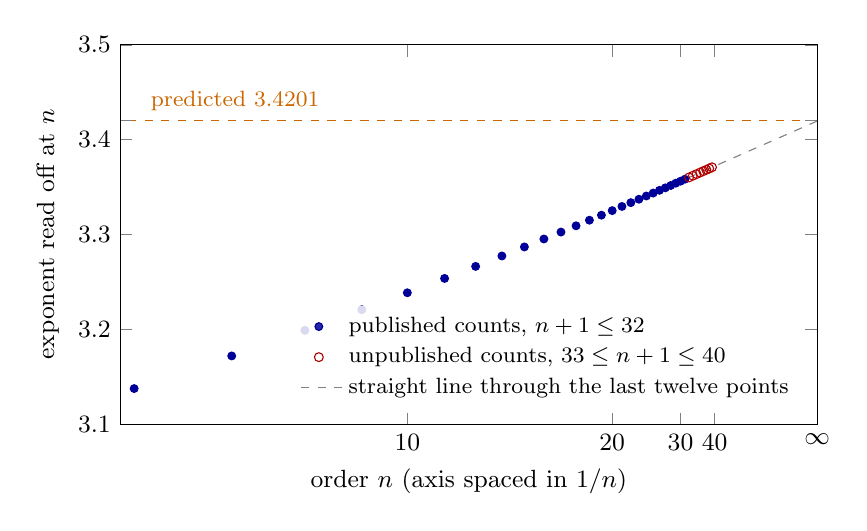
\begin{tikzpicture}
\begin{axis}[width=0.86\textwidth,height=6.4cm,xmin=0,xmax=0.17,ymin=3.1,ymax=3.5,x dir=reverse,
  xlabel={order $n$ (axis spaced in $1/n$)},ylabel={exponent read off at $n$},
  xtick={0,0.025,0.03333,0.05,0.1},xticklabels={$\infty$,$40$,$30$,$20$,$10$},
  extra y ticks={3.4201},extra y tick labels={},extra y tick style={grid=major,grid style={dashed,orange!80!black}},
  legend image post style={xscale=-1},legend cell align=left,
  legend style={font=\footnotesize,at={(0.98,0.04)},anchor=south east,draw=none,fill=white,fill opacity=0.85,text opacity=1},
  tick label style={font=\small},label style={font=\small}]
\addplot[only marks,mark=*,mark size=1.4pt,blue!60!black] coordinates {(0.16667,3.1377) (0.14286,3.1721) (0.12500,3.1991) (0.11111,3.2208) (0.10000,3.2387) (0.09091,3.2538) (0.08333,3.2665) (0.07692,3.2775) (0.07143,3.2870) (0.06667,3.2954) (0.06250,3.3027) (0.05882,3.3093) (0.05556,3.3152) (0.05263,3.3205) (0.05000,3.3253) (0.04762,3.3297) (0.04545,3.3337) (0.04348,3.3373) (0.04167,3.3407) (0.04000,3.3438) (0.03846,3.3467) (0.03704,3.3493) (0.03571,3.3518) (0.03448,3.3542) (0.03333,3.3563) (0.03226,3.3584)};
\addlegendentry{published counts, $n+1\le32$}
\addplot[only marks,mark=o,mark size=1.6pt,red!70!black] coordinates {(0.03125,3.3603) (0.03030,3.3621) (0.02941,3.3638) (0.02857,3.3654) (0.02778,3.3669) (0.02703,3.3683) (0.02632,3.3697) (0.02564,3.3710)};
\addlegendentry{unpublished counts, $33\le n+1\le40$}
\addplot[dashed,gray,domain=0:0.045] {3.4197-1.9010*x};
\addlegendentry{straight line through the last twelve points}
\node[font=\footnotesize,orange!80!black,anchor=south west] at (axis cs:0.165,3.4201) {predicted $3.4201$};
\end{axis}
\end{tikzpicture}
\caption{The exponent read off from consecutive exact counts $M_n$ and $M_{n+1}$,
$6\le n\le 39$, using the numerical estimate $\mu=12.262874$. Filled dots use published counts
($n+1\le 32$)~\cite{JG,JensenGit}. Open circles use the counts for $33\le n+1\le 40$, which were
computed privately and have not been published or independently checked. The gray line, fitted
through the last twelve points, is only a guide to the eye.}
\label{fig:readoff}
\end{figure}

This is a picture, not a measurement. Careful fits with several correction terms are consistent
with $\alpha_*$ to about three decimal places: Jensen and Guttmann estimated
$\alpha=3.4208\pm0.0006$~\cite{JG}, and a fit in this project to all $40$ counts gives
$3.4205\pm0.0004$ (Appendix~\ref{app:repo}). The second fit uses the counts for $33\le n\le40$,
which have not been checked. The data are consistent with a polynomial correction whose exponent differs from $3$, the
value for pairs of arch systems. The existence of such an asymptotic correction remains unproved.

\subsection{A meander as a walk in the quarter plane}\label{sec:quarter}

There is an appealing shortcut to $\alpha$, and it is instructive to see why it fails. Draw a
vertical line between two crossings and record two numbers: the number of arches
below the river and the number above the river that cross the line. Each crossing changes each
number by one, so a meander becomes a walk in the quarter plane that starts and ends near the
corner.

For pairs of arch systems without the one-loop requirement, the two coordinates are two
independent walks of the kind in~\eqref{eq:catalan}, and the exponent $3=3/2+3/2$ follows. More
generally, consider walks with small independent steps in the quarter plane whose two coordinates
have correlation $r$. The number of such walks that stay in the quarter plane and return to the
corner decays with the exponent $1+\pi/\arccos(-r)$~\cite{DW}; at $r=0$ this is $3$. The meander value $3.4201$ would
need $r\approx -0.27$. One could try to measure the correlation in meanders and read off the
exponent. This does not work, for two reasons.

\begin{itemize}
\item The correlation is not $-0.27$. In sampled meanders of order $512$ it is about $-0.19$
for single steps and about $-0.08$ over blocks of $8$ to $64$ steps.
\item The available measurements do not justify a Brownian approximation. Over the sampled range,
the typical size is fitted by $n^{0.52}$; finite-size data alone cannot determine the limiting scaling.
\end{itemize}

The two numbers forget how the open arches are joined to each other, and whether a crossing
closes a loop too early depends on exactly that. The walk organizes computations, but it does not
determine the exponent.

\subsection{The tape machine}\label{sec:tape}

The quarter-plane walk forgets how the open arches are joined. Paper~B~\cite{PaperB} keeps exactly
the information that matters, in a short word in two letters called the \emph{tape}.
Figure~\ref{fig:film} shows the idea before any definitions.

Draw a vertical line, the \emph{sweep line}, between two neighboring crossings and cover
everything to its right. Intuitively, this is like sliding a piece of paper from left to right along the
meander, stopping between two crossings. The sweep line meets a few pieces of road below the river, then
the river itself, then a few pieces of road above. These pieces of road are the \emph{open}
arches: they have started but not yet ended. Each object met by the sweep line gets a letter, \tape{+}
or \tape{-}, and reading the letters from bottom to top gives the tape. The letter on the river
is marked with a square in the figure and with brackets in the text; it is the \emph{head}. As
the paper slides past one more crossing, the tape changes only next to the head.

\begin{figure}[ht]
\centering
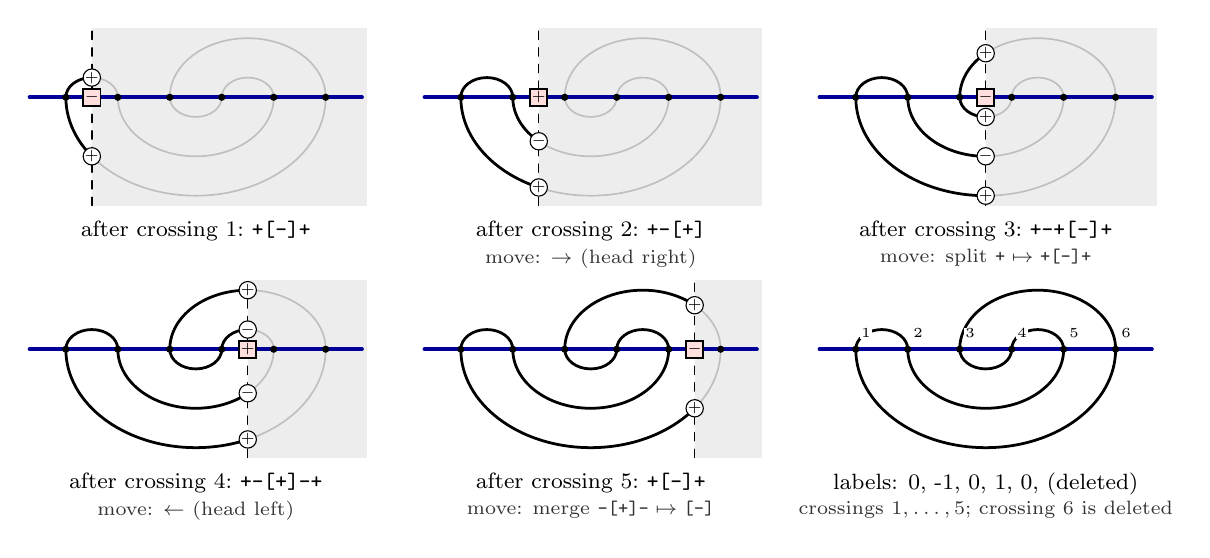
\begin{tikzpicture}[x=0.66cm,y=0.5cm,line cap=round]
\begin{scope}[shift={(0.00,0.00)}]
  \fill[black!7] (1.50,-2.75) rectangle (6.8,1.75);
  \draw[blue!60!black,line width=1.3pt] (0.3,0)--(6.7,0);
  \begin{scope}[black!25,line width=0.6pt]\meanderroad\end{scope}
  \begin{scope}\clip (0.3,-2.75) rectangle (1.50,1.75);\begin{scope}[line width=1pt]\meanderroad\end{scope}\end{scope}
  \draw[dashed,line width=0.5pt] (1.50,-2.75)--(1.50,1.75);
  \foreach \k in {1,...,6} {\fill (\k,0) circle[radius=1.3pt];}
  \draw[fill=white,line width=0.4pt] (1.50,-1.500) circle[radius=0.11cm]; \node[font=\tiny,inner sep=0pt] at (1.50,-1.500) {$+$};
  \draw[fill=red!13,line width=0.7pt] (1.50,0) ++(-0.11cm,-0.11cm) rectangle ++(0.22cm,0.22cm); \node[font=\tiny,inner sep=0pt] at (1.50,0) {$-$};
  \draw[fill=white,line width=0.4pt] (1.50,0.500) circle[radius=0.11cm]; \node[font=\tiny,inner sep=0pt] at (1.50,0.500) {$+$};
  \node[font=\footnotesize,anchor=north] at (3.5,-2.9) {after crossing 1:\ \tape{+}\hd{-}\tape{+}};
\end{scope}
\begin{scope}[shift={(7.60,0.00)}]
  \fill[black!7] (2.50,-2.75) rectangle (6.8,1.75);
  \draw[blue!60!black,line width=1.3pt] (0.3,0)--(6.7,0);
  \begin{scope}[black!25,line width=0.6pt]\meanderroad\end{scope}
  \begin{scope}\clip (0.3,-2.75) rectangle (2.50,1.75);\begin{scope}[line width=1pt]\meanderroad\end{scope}\end{scope}
  \draw[dashed,line width=0.5pt] (2.50,-2.75)--(2.50,1.75);
  \foreach \k in {1,...,6} {\fill (\k,0) circle[radius=1.3pt];}
  \draw[fill=white,line width=0.4pt] (2.50,-2.291) circle[radius=0.11cm]; \node[font=\tiny,inner sep=0pt] at (2.50,-2.291) {$+$};
  \draw[fill=white,line width=0.4pt] (2.50,-1.118) circle[radius=0.11cm]; \node[font=\tiny,inner sep=0pt] at (2.50,-1.118) {$-$};
  \draw[fill=red!13,line width=0.7pt] (2.50,0) ++(-0.11cm,-0.11cm) rectangle ++(0.22cm,0.22cm); \node[font=\tiny,inner sep=0pt] at (2.50,0) {$+$};
  \node[font=\footnotesize,anchor=north] at (3.5,-2.9) {after crossing 2:\ \tape{+}\tape{-}\hd{+}};
  \node[font=\scriptsize,anchor=north,gray!40!black] at (3.5,-3.6) {move: $\to$ (head right)};
\end{scope}
\begin{scope}[shift={(15.20,0.00)}]
  \fill[black!7] (3.50,-2.75) rectangle (6.8,1.75);
  \draw[blue!60!black,line width=1.3pt] (0.3,0)--(6.7,0);
  \begin{scope}[black!25,line width=0.6pt]\meanderroad\end{scope}
  \begin{scope}\clip (0.3,-2.75) rectangle (3.50,1.75);\begin{scope}[line width=1pt]\meanderroad\end{scope}\end{scope}
  \draw[dashed,line width=0.5pt] (3.50,-2.75)--(3.50,1.75);
  \foreach \k in {1,...,6} {\fill (\k,0) circle[radius=1.3pt];}
  \draw[fill=white,line width=0.4pt] (3.50,-2.500) circle[radius=0.11cm]; \node[font=\tiny,inner sep=0pt] at (3.50,-2.500) {$+$};
  \draw[fill=white,line width=0.4pt] (3.50,-1.500) circle[radius=0.11cm]; \node[font=\tiny,inner sep=0pt] at (3.50,-1.500) {$-$};
  \draw[fill=white,line width=0.4pt] (3.50,-0.500) circle[radius=0.11cm]; \node[font=\tiny,inner sep=0pt] at (3.50,-0.500) {$+$};
  \draw[fill=red!13,line width=0.7pt] (3.50,0) ++(-0.11cm,-0.11cm) rectangle ++(0.22cm,0.22cm); \node[font=\tiny,inner sep=0pt] at (3.50,0) {$-$};
  \draw[fill=white,line width=0.4pt] (3.50,1.118) circle[radius=0.11cm]; \node[font=\tiny,inner sep=0pt] at (3.50,1.118) {$+$};
  \node[font=\footnotesize,anchor=north] at (3.5,-2.9) {after crossing 3:\ \tape{+}\tape{-}\tape{+}\hd{-}\tape{+}};
  \node[font=\scriptsize,anchor=north,gray!40!black] at (3.5,-3.6) {move: split $\tape{+}\mapsto\tape{+}\hd{-}\tape{+}$};
\end{scope}
\begin{scope}[shift={(0.00,-6.40)}]
  \fill[black!7] (4.50,-2.75) rectangle (6.8,1.75);
  \draw[blue!60!black,line width=1.3pt] (0.3,0)--(6.7,0);
  \begin{scope}[black!25,line width=0.6pt]\meanderroad\end{scope}
  \begin{scope}\clip (0.3,-2.75) rectangle (4.50,1.75);\begin{scope}[line width=1pt]\meanderroad\end{scope}\end{scope}
  \draw[dashed,line width=0.5pt] (4.50,-2.75)--(4.50,1.75);
  \foreach \k in {1,...,6} {\fill (\k,0) circle[radius=1.3pt];}
  \draw[fill=white,line width=0.4pt] (4.50,-2.291) circle[radius=0.11cm]; \node[font=\tiny,inner sep=0pt] at (4.50,-2.291) {$+$};
  \draw[fill=white,line width=0.4pt] (4.50,-1.118) circle[radius=0.11cm]; \node[font=\tiny,inner sep=0pt] at (4.50,-1.118) {$-$};
  \draw[fill=red!13,line width=0.7pt] (4.50,0) ++(-0.11cm,-0.11cm) rectangle ++(0.22cm,0.22cm); \node[font=\tiny,inner sep=0pt] at (4.50,0) {$+$};
  \draw[fill=white,line width=0.4pt] (4.50,0.500) circle[radius=0.11cm]; \node[font=\tiny,inner sep=0pt] at (4.50,0.500) {$-$};
  \draw[fill=white,line width=0.4pt] (4.50,1.500) circle[radius=0.11cm]; \node[font=\tiny,inner sep=0pt] at (4.50,1.500) {$+$};
  \node[font=\footnotesize,anchor=north] at (3.5,-2.9) {after crossing 4:\ \tape{+}\tape{-}\hd{+}\tape{-}\tape{+}};
  \node[font=\scriptsize,anchor=north,gray!40!black] at (3.5,-3.6) {move: $\leftarrow$ (head left)};
\end{scope}
\begin{scope}[shift={(7.60,-6.40)}]
  \fill[black!7] (5.50,-2.75) rectangle (6.8,1.75);
  \draw[blue!60!black,line width=1.3pt] (0.3,0)--(6.7,0);
  \begin{scope}[black!25,line width=0.6pt]\meanderroad\end{scope}
  \begin{scope}\clip (0.3,-2.75) rectangle (5.50,1.75);\begin{scope}[line width=1pt]\meanderroad\end{scope}\end{scope}
  \draw[dashed,line width=0.5pt] (5.50,-2.75)--(5.50,1.75);
  \foreach \k in {1,...,6} {\fill (\k,0) circle[radius=1.3pt];}
  \draw[fill=white,line width=0.4pt] (5.50,-1.500) circle[radius=0.11cm]; \node[font=\tiny,inner sep=0pt] at (5.50,-1.500) {$+$};
  \draw[fill=red!13,line width=0.7pt] (5.50,0) ++(-0.11cm,-0.11cm) rectangle ++(0.22cm,0.22cm); \node[font=\tiny,inner sep=0pt] at (5.50,0) {$-$};
  \draw[fill=white,line width=0.4pt] (5.50,1.118) circle[radius=0.11cm]; \node[font=\tiny,inner sep=0pt] at (5.50,1.118) {$+$};
  \node[font=\footnotesize,anchor=north] at (3.5,-2.9) {after crossing 5:\ \tape{+}\hd{-}\tape{+}};
  \node[font=\scriptsize,anchor=north,gray!40!black] at (3.5,-3.6) {move: merge $\tape{-}\hd{+}\tape{-}\mapsto\hd{-}$};
\end{scope}
\begin{scope}[shift={(15.20,-6.40)}]
  \draw[blue!60!black,line width=1.3pt] (0.3,0)--(6.7,0);
  \begin{scope}[line width=1pt]\meanderroad\end{scope}
  \foreach \k in {1,...,6} {\fill (\k,0) circle[radius=1.3pt]; \node[fill=white,inner sep=0.5pt,font=\tiny] at (\k+0.2,0.4) {\k};}
  \node[font=\footnotesize,anchor=north] at (3.5,-2.9) {labels: 0,\ -1,\ 0,\ 1,\ 0,\ (deleted)};
  \node[font=\scriptsize,anchor=north,gray!40!black] at (3.5,-3.6) {crossings $1,\dots,5$; crossing $6$ is deleted};
\end{scope}
\end{tikzpicture}

\caption{The tape machine on the meander of Figure~\ref{fig:meander}. In each panel the part of
the meander right of the dashed sweep line is covered (gray). The sweep line meets the open arches below the
river, the river (square: the head), and the open arches above; their letters, read from bottom
to top, form the tape. Passing one crossing changes the tape by one move, named under each panel.
The last panel shows the labels from which the letters are computed.}
\label{fig:film}
\end{figure}

The letters come from a numbering of the crossings. Delete the last crossing; the road, which
was a closed loop, becomes a single path through the other crossings. Give the first crossing the
\emph{label} $0$ and walk along the path: the label drops by one along an arch above the river,
read from left to right, and rises by one along an arch below the river. Intuitively, the label
counts the half turns of the road, with turns above and below the river counted with opposite
signs. A planar argument shows that neighboring crossings along the river have labels that differ
by exactly one. Now give each gap between two objects on the sweep line a number: $-1$ for the gap below
everything, $0$ for the gap above everything, the label of its left end for the gap just above
an open arch below the river, and that label minus one for the gap just below an open arch above
the river. Neighboring gap numbers differ by exactly one, and the letter of each object says
whether the number goes up (\tape{+}) or down (\tape{-}) across it.

\begin{theorem}[the tape machine~\cite{PaperB}]\label{thm:tape}
A \emph{tape} is a word in \tape{+} and \tape{-} with one marked letter, the head, written in
brackets. A \emph{move} does one of the following: move the head one letter left or right; replace
a head \tape{+} by \tape{+}\hd{-}\tape{+}; replace a head \tape{-} by \tape{+}\hd{-}\tape{-} or by
\tape{-}\hd{-}\tape{+}; or replace a head \tape{+} together with its two neighbors by a single
head letter, which is \tape{-} if both neighbors are \tape{-} and \tape{+} otherwise. This last
move is not allowed when both neighbors are \tape{+}, that is, at \tape{+}\hd{+}\tape{+}. Then
the meanders of order $n$ are in one-to-one correspondence with the sequences of $2n-2$ moves that
start at the tape \tape{+}\hd{-}\tape{+} and end at it.
\end{theorem}

\begin{figure}[t]
\centering
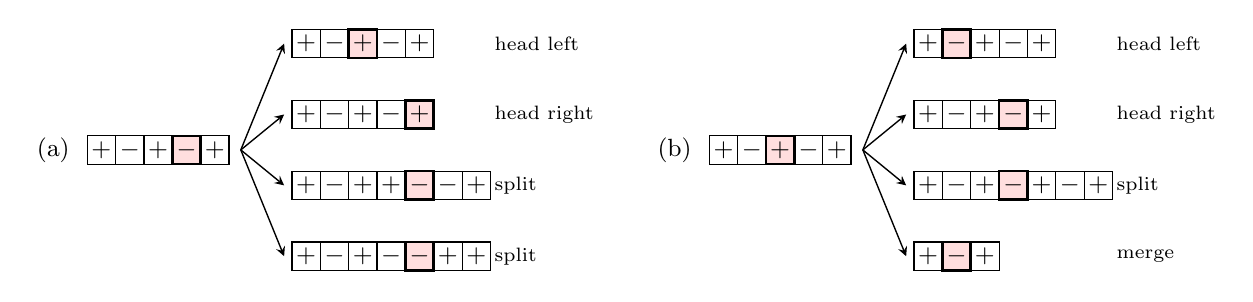
\begin{tikzpicture}[>=stealth]
  \tp{(0,0)}{+,-,+,-,+}{4}
  \tp{(2.6,1.35)}{+,-,+,-,+}{3} \draw[->,line width=0.5pt] (1.95,0)--(2.5,1.35); \node[font=\scriptsize,anchor=west] at (5.05,1.35) {head left};
  \tp{(2.6,0.45)}{+,-,+,-,+}{5} \draw[->,line width=0.5pt] (1.95,0)--(2.5,0.45); \node[font=\scriptsize,anchor=west] at (5.05,0.45) {head right};
  \tp{(2.6,-0.45)}{+,-,+,+,-,-,+}{5} \draw[->,line width=0.5pt] (1.95,0)--(2.5,-0.45); \node[font=\scriptsize,anchor=west] at (5.05,-0.45) {split};
  \tp{(2.6,-1.35)}{+,-,+,-,-,+,+}{5} \draw[->,line width=0.5pt] (1.95,0)--(2.5,-1.35); \node[font=\scriptsize,anchor=west] at (5.05,-1.35) {split};
  \node[font=\small,anchor=east] at (-0.1,0) {(a)};
  \begin{scope}[xshift=7.9cm]
  \tp{(0,0)}{+,-,+,-,+}{3}
  \tp{(2.6,1.35)}{+,-,+,-,+}{2} \draw[->,line width=0.5pt] (1.95,0)--(2.5,1.35); \node[font=\scriptsize,anchor=west] at (5.05,1.35) {head left};
  \tp{(2.6,0.45)}{+,-,+,-,+}{4} \draw[->,line width=0.5pt] (1.95,0)--(2.5,0.45); \node[font=\scriptsize,anchor=west] at (5.05,0.45) {head right};
  \tp{(2.6,-0.45)}{+,-,+,-,+,-,+}{4} \draw[->,line width=0.5pt] (1.95,0)--(2.5,-0.45); \node[font=\scriptsize,anchor=west] at (5.05,-0.45) {split};
  \tp{(2.6,-1.35)}{+,-,+}{2} \draw[->,line width=0.5pt] (1.95,0)--(2.5,-1.35); \node[font=\scriptsize,anchor=west] at (5.05,-1.35) {merge};
  \node[font=\small,anchor=east] at (-0.1,0) {(b)};
  \end{scope}
\end{tikzpicture}
\caption{All moves from two tapes of Figure~\ref{fig:film}; the shaded box is the head.
(a) From \tape{+-+}\hd{-}\tape{+} (after crossing $3$), with the head on a \tape{-}: two head
moves and two splits. (b) From \tape{+-}\hd{+}\tape{-+} (after crossing $4$), with the head on a
\tape{+}: two head moves, one split, and the merge, which returns to the starting tape.}
\label{fig:moves}
\end{figure}

The moves match the four kinds of crossing. A crossing opens or closes one arch above and one
below the river. Opening on one side and closing on the other moves the head; opening on both
sides replaces one letter by three (a \emph{split}); closing on both sides replaces three letters
by one (a \emph{merge}). Figure~\ref{fig:moves} shows every move available at two tapes. The first
crossing creates the starting tape and the last closes the final two arches, so a meander of order
$n$, with $2n$ crossings, gives $2n-2$ moves. In Figure~\ref{fig:film} the four moves are head
right, split, head left and merge.

Each move reads and changes only the head and its two neighbors, so the global one-loop condition
has become a set of local rules. The merge at \tape{+}\hd{+}\tape{+} is excluded because no
consistent labels could follow it: after it, the open arches would force the next label to go
down and up at once. Conversely, a planar argument shows that labels obeying the local rules always
come from a single closed road. For $n=2$ there are exactly two sequences,
\[ \tape{+}\hd{-}\tape{+} \to \hd{+}\tape{-+} \to \tape{+}\hd{-}\tape{+}
\qquad\text{and}\qquad
\tape{+}\hd{-}\tape{+} \to \tape{+-}\hd{+} \to \tape{+}\hd{-}\tape{+},\]
matching the two meanders of order $2$. Enumerating the sequences by computer reproduces
$1, 2, 8, 42, 262, 1828$ for $n\le 6$.

In this picture $M_n$ literally counts walks that come back to their start, as in the first
subsection: walks on the set of tapes. The growth rate $\mu$ is the growth rate of the number of
such walks, and $\alpha$ is the conjectured power-law correction after the factor $\mu^n$ is removed. But the set
of tapes is infinite, and the walk is not close to a Brownian motion, which is why the reasoning
of the first subsection does not produce $\alpha$ directly.

The tape machine is behind the best current bounds on $\mu$, proved in Paper~B,
\[ 12.2191\;\le\;\mu\;\le\;12.2970 .\]
The upper bound uses two positive weights, one looking forward along the moves and one looking
backward. Their paired inequalities control a symmetric operator on every finite set of tapes.
This bounds the number of closed move sequences, and hence the exponential growth of $M_n$,
by $12.2970$ per order.
The lower bound comes from a random rule for choosing moves that looks only at the letters near
the head, keeps the tape statistically the same over time, and on average neither lengthens the
tape nor moves the head to one side. Its \emph{entropy}, the average over the choices it makes
of the logarithm of one over the probability of the choice, is at least $\log 12.2191$ per two
moves. Intuitively, such a rule makes in effect about $12.2191$ equally likely choices per two
moves, so it produces about $12.2191^n$ different sequences of $2n$ moves. These sequences can be
closed into meanders at small cost, which gives $\mu\ge12.2191$. Both certificates were checked in exact arithmetic, and each was checked again by a
separately written program; for the lower bound, part of this second check covers a sample of
the equations rather than all of them. Paper~B explains both certificates; it supersedes an
earlier account of the weight method in this project~\cite{BoundsPaper}. The best bounds
published in a journal are $11.380\le\mu\le12.901$~\cite{AP}, and recent certified computations
and preprints give $11.6080\le\mu\le12.6319$~\cite{Fox} and $\mu\le12.806$~\cite{CDDV}.

\subsection{Meanders with bounded labels}\label{sec:band}

Restricting the labels to a fixed range makes the machine much simpler, and then the exponent
can be computed exactly. For the meanders whose labels all lie between $-1$ and $2$ the following
holds; the proof is in Paper~C~\cite{PaperC}.

\begin{theorem}[meanders with labels in $\{-1,0,1,2\}$]\label{thm:band}
Let $m_0=0.9175\ldots$ be the positive root of $4x^4=2x+1$. The number of meanders of order $n$
with all labels in $\{-1,0,1,2\}$ grows like $\Lambda^n$, where
$\Lambda=(1+2m_0)(1+m_0)^2=10.4245\ldots$ is the larger real root of
$16x^4-112x^3-520x^2-536x+25$. More precisely, the number is $\Lambda^n n^{-\alpha_{\mathrm b}+o(1)}$, where
\[ \alpha_{\mathrm b} \;=\; 1+\frac{\pi}{\arccos\!\big((1+2m_0)/(3+4m_0)\big)} \;=\; 3.7758\ldots \]
\end{theorem}

The exponent has the same form as the quarter-plane return exponent above: one plus $\pi$
divided by an angle. With the labels bounded, the machine has only finitely many control states,
and the two coordinates of Section~\ref{sec:quarter}, the numbers of open arches below and above
the river, behave at large scales like a planar Brownian motion with correlated coordinates. A
linear change of coordinates turns it into a standard Brownian motion and turns the quarter plane
into a wedge with opening angle $\arccos\big((1+2m_0)/(3+4m_0)\big)$, and this angle sets the
exponent. Like $\alpha_*$, the value $\alpha_{\mathrm b}$ is irrational, but for a different
reason: it comes from an angle, not from the root of a quadratic equation. For all meanders the
labels are unbounded, and no reduction of this kind is known.

%%%%%%%%%%%%%%%%%%%%%%%%%%%%%%%%%%%%%%%%%%%%%%%%%%%%%%%%%%%%%%%%%%%%%%%%
\section{Meanders as random surfaces}\label{sec:surfaces}
%%%%%%%%%%%%%%%%%%%%%%%%%%%%%%%%%%%%%%%%%%%%%%%%%%%%%%%%%%%%%%%%%%%%%%%%

This section explains the physical argument behind~\eqref{eq:alpha}. Each step is either a
theorem about simpler objects or a prediction, and we say which.

\subsection{A sphere made of squares}

Turn each crossing of the river and the road into a small square tile. The river enters and
leaves the tile through two opposite sides, and the road through the other two
(Figure~\ref{fig:tile}). When two crossings are neighbors along the river, glue their tiles
along the sides through which the river passes from one to the other, and do the same for
neighbors along the road. The river is an infinite straight line; add a point at infinity, so
that the plane becomes a sphere and the river becomes a closed loop. With this, every side of
every tile is glued to a side of another tile, and the tiles form a closed surface shaped like a
sphere.

\begin{figure}[t]
\centering
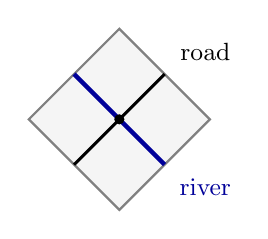
\begin{tikzpicture}[scale=1.15]
  \draw[gray,line width=0.8pt,fill=gray!8] (0,1)--(1,0)--(0,-1)--(-1,0)--cycle;
  \draw[blue!60!black,line width=1.6pt] (-0.5,0.5)--(0.5,-0.5);
  \draw[line width=1.1pt] (0.5,0.5)--(-0.5,-0.5);
  \fill (0,0) circle[radius=1.6pt];
  \node[blue!60!black,font=\small] at (0.95,-0.75) {river};
  \node[font=\small] at (0.95,0.75) {road};
\end{tikzpicture}
\caption{One crossing becomes one square tile; the river and the road each pass through it once.
Gluing the tiles of all $2n$ crossings gives a sphere made of $2n$ squares, with two curves drawn
on it that each pass through every square once.}
\label{fig:tile}
\end{figure}

So a meander of order $n$ is a sphere built from $2n$ squares, together with two curves on it,
the river and the road, each of which passes through every square exactly once. Counting
meanders means counting such decorated spheres.

\subsection{Random surfaces without drawings}

The sphere of squares can also be drawn directly from the picture of the meander, and this is
the easiest way to see what kind of object it is (Figure~\ref{fig:spheres}). The river and the
road cut the plane into regions; recall that the river is closed up through a point at infinity,
so the region above the river and the region below it at infinity are different. Put a dot in each
region. Each piece of river or road between two crossings separates two regions; join their dots
by an edge that crosses that piece. Each crossing is then surrounded by exactly four edges, so it
becomes a square, and these squares are the tiles of Figure~\ref{fig:tile}. A meander of order $n$
gives $2n+2$ dots, $4n$ edges and $2n$ squares. For the meander of order~$2$ in
Figure~\ref{fig:spheres}(a), the six regions $v_1,\ldots,v_6$ give the sphere in panel~(b): two
points $v_1$ and $v_6$ joined by four paths of length two, through $v_2$, $v_3$, $v_4$ and $v_5$,
with a square between each pair of neighboring paths (one of them is the outside of the
picture).

\begin{figure}[t]
\centering
% Spheres of squares from meanders (Section 3.2). Regions of the plane become vertices,
% pieces of river and road become edges, crossings become square faces.
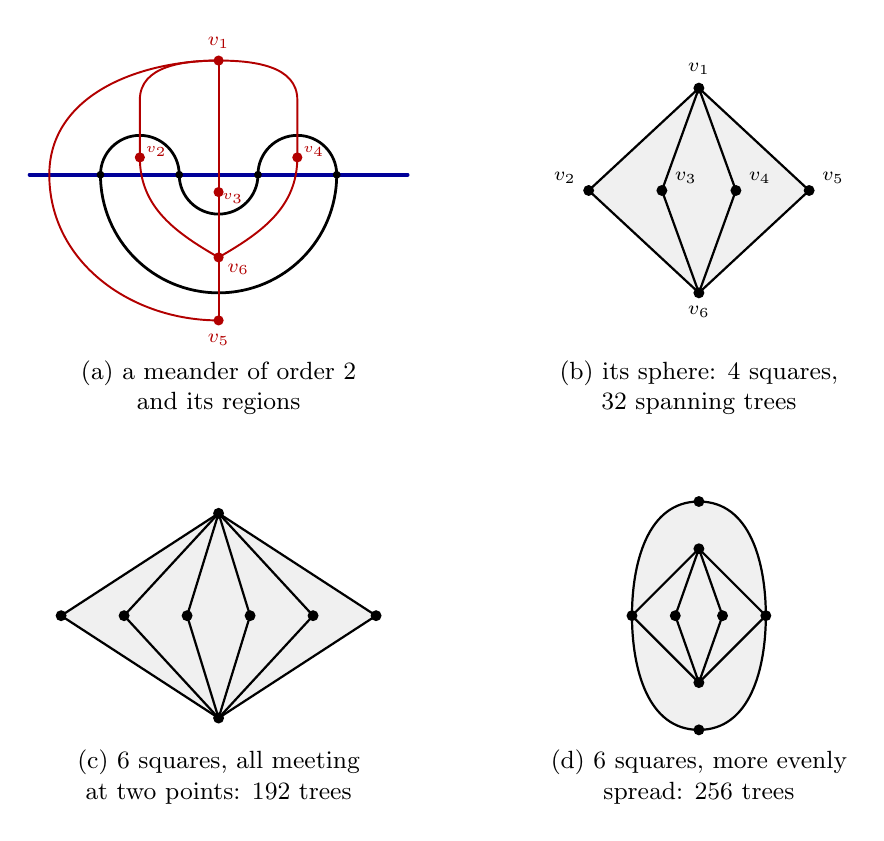
\begin{tikzpicture}[line cap=round]
  \tikzset{reg/.style={circle,fill=red!70!black,inner sep=1.3pt},
           dual/.style={red!70!black,line width=0.7pt},
           qv/.style={circle,fill=black,inner sep=1.4pt},
           qe/.style={line width=0.8pt},
           lab/.style={font=\scriptsize}}
  % ---------- (a) meander of order 2 with its regions ----------
  \begin{scope}[x=1cm,y=1cm]
    \draw[blue!60!black,line width=1.4pt] (0.1,0)--(4.9,0);
    \begin{scope}[line width=1pt]
      \draw (1,0) arc[start angle=180,end angle=0,radius=0.5];
      \draw (3,0) arc[start angle=180,end angle=0,radius=0.5];
      \draw (1,0) arc[start angle=180,end angle=360,radius=1.5];
      \draw (2,0) arc[start angle=180,end angle=360,radius=0.5];
    \end{scope}
    \foreach \k in {1,...,4} \fill (\k,0) circle[radius=1.4pt];
    % dual edges
    \draw[dual] (1.5,0.22)--(1.5,0.95) to[out=90,in=180] (2.5,1.45);
    \draw[dual] (3.5,0.22)--(3.5,0.95) to[out=90,in=0] (2.5,1.45);
    \draw[dual] (2.5,1.45)--(2.5,-0.22);
    \draw[dual] (1.5,0.22) to[out=-90,in=150] (2.5,-1.05);
    \draw[dual] (3.5,0.22) to[out=-90,in=30] (2.5,-1.05);
    \draw[dual] (2.5,-0.22)--(2.5,-1.05)--(2.5,-1.85);
    \draw[dual] (2.5,1.45) to[out=180,in=90] (0.35,0) to[out=-90,in=180] (2.5,-1.85);
    \foreach \p/\n/\a in {(1.5,0.22)/A/north,(3.5,0.22)/B/north,(2.5,1.45)/U/south,(2.5,-0.22)/C/east,(2.5,-1.05)/D/east,(2.5,-1.85)/L/north} {
      \node[reg] at \p {}; }
    \node[lab,font=\tiny,red!70!black] at (1.71,0.29) {$v_2$};
    \node[lab,font=\tiny,red!70!black] at (3.71,0.29) {$v_4$};
    \node[lab,red!70!black] at (2.5,1.68) {$v_1$};
    \node[lab,font=\tiny,red!70!black] at (2.68,-0.30) {$v_3$};
    \node[lab,red!70!black] at (2.75,-1.2) {$v_6$};
    \node[lab,red!70!black] at (2.5,-2.1) {$v_5$};
    \node[font=\small,align=center] at (2.5,-2.7) {(a) a meander of order $2$\\ and its regions};
  \end{scope}
  % ---------- (b) its sphere: four squares ----------
  \begin{scope}[xshift=8.6cm,yshift=-0.2cm]
    \fill[gray!12] (0,1.3)--(-1.4,0)--(0,-1.3)--(1.4,0)--cycle;
    \foreach \x/\n/\dx/\an in {-1.4/2/-0.04/east,-0.47/3/0.04/west,0.47/4/0.04/west,1.4/5/0.04/west} {
      \draw[qe] (0,1.3)--(\x,0)--(0,-1.3);
      \node[qv] at (\x,0) {}; \node[lab,anchor=\an] at (\x+\dx,0.16) {$v_\n$};}
    \node[qv] at (0,1.3) {}; \node[lab,anchor=south] at (0,1.35) {$v_1$};
    \node[qv] at (0,-1.3) {}; \node[lab,anchor=north] at (0,-1.35) {$v_6$};
    \node[font=\small,align=center] at (0,-2.5) {(b) its sphere: $4$ squares,\\ $32$ spanning trees};
  \end{scope}
  % ---------- (c) the six-square sphere where all squares meet at two points ----------
  \begin{scope}[yshift=-5.6cm,xshift=2.5cm]
    \fill[gray!12] (0,1.3)--(-2.0,0)--(0,-1.3)--(2.0,0)--cycle;
    \foreach \x in {-2.0,-1.2,-0.4,0.4,1.2,2.0} {
      \draw[qe] (0,1.3)--(\x,0)--(0,-1.3); \node[qv] at (\x,0) {};}
    \node[qv] at (0,1.3) {}; \node[qv] at (0,-1.3) {};
    \node[font=\small,align=center] at (0,-2.05) {(c) $6$ squares, all meeting\\ at two points: $192$ trees};
  \end{scope}
  % ---------- (d) the six-square sphere of the meander of Figure 1 ----------
  \begin{scope}[yshift=-5.6cm,xshift=8.6cm]
    \coordinate (U) at (0,0.85); \coordinate (C) at (0.85,0); \coordinate (G) at (0,-0.85); \coordinate (E) at (-0.85,0);
    \fill[gray!12] (C) to[out=90,in=0] (0,1.45) to[out=180,in=90] (E) to[out=-90,in=180] (0,-1.45) to[out=0,in=-90] (C);
    \draw[qe] (U)--(C)--(G)--(E)--cycle;
    \draw[qe] (U)--(-0.3,0)--(G);
    \draw[qe] (U)--(0.3,0)--(G);
    \draw[qe] (C) to[out=90,in=0] (0,1.45) to[out=180,in=90] (E);
    \draw[qe] (C) to[out=-90,in=0] (0,-1.45) to[out=180,in=-90] (E);
    \foreach \p in {(U),(C),(G),(E),(0,1.45),(0,-1.45),(-0.3,0),(0.3,0)} \node[qv] at \p {};
    \node[font=\small,align=center] at (0,-2.05) {(d) $6$ squares, more evenly\\ spread: $256$ trees};
  \end{scope}
\end{tikzpicture}

\caption{From a meander to a sphere of squares. (a) The meander of order $2$ whose upper arches
join $1$--$2$ and $3$--$4$ and whose lower arches join $1$--$4$ and $2$--$3$. Each region gets a
dot, and each piece of river or road becomes an edge (red) between the dots on its two sides.
(b) The resulting sphere, redrawn: each crossing has become a square, and the outside of the
picture is the fourth square. (c), (d) Two spheres of six squares that come from meanders of
order $3$; (d) comes from the meander of Figure~\ref{fig:meander}. They carry $192$ and $256$
spanning trees.}
\label{fig:spheres}
\end{figure}

A graph drawn on the sphere without crossings, considered up to deformation, is called a
\emph{planar map}. Its \emph{faces} are the regions into which the edges cut the sphere, and a
sphere glued from squares is a planar map in which every face has four sides. Not every such
sphere comes from a meander, since a meander also carries the river and the road, but every
sphere of squares is a random-surface model in its own right. Such spheres, with nothing drawn on
them, are well understood. Tutte counted them in the 1960s~\cite{Tutte}: with one marked edge
(which removes symmetries), the numbers with $1,2,3,4,5$ squares are $2, 9, 54, 378, 2916$, and
with $n$ squares there are about
\[ 12^n\, n^{-5/2} \]
of them. Here $n$ counts squares, while a meander of order $n$ has $2n$ squares; the exponent
does not depend on this choice of scale. Glued from triangles instead, the count grows at a
different rate but with the same power $n^{-5/2}$. This is universality again, now for surfaces.
Zoomed out, a uniformly random sphere glued from many squares, or from many triangles, looks like
one and the same random surface, called the \emph{Brownian map}; it plays the role that Brownian
motion plays for walks~\cite{LeGall,Miermont}.

In physics, a sum over random geometries of space is called a theory of \emph{quantum gravity}.
In two dimensions a geometry is just a surface, so ``two-dimensional quantum gravity'' means
nothing more than a random surface. No actual gravity is involved, and the name is used below
only when quoting the physics literature.

\subsection{One drawing: a spanning tree}

Now draw something on the surface and count surfaces together with drawings. The simplest case
is a \emph{spanning tree}: a set of edges that connects every vertex without closing any loop.
Mullin showed that the planar maps with $n$ edges and a marked spanning tree number exactly
$\mathrm{Cat}_n\mathrm{Cat}_{n+1}$~\cite{Mullin}, so about
\[ 16^n\, n^{-3} \]
up to a constant factor (again with one marked edge). The exponent has moved from $5/2$ to $3$.
The proof explains why. A map with a spanning tree can be read as two interleaved bracket words,
one for the tree and one for the edges outside it; a \emph{bracket word} is a sequence of opening
and closing brackets that match up, like the arch systems above. Each word is a walk that comes
back and stays above its start, so the exponent is $3/2+3/2$.

A meander carries two drawings, the river and the road. Each is a single curve that visits
every square once. Physicists expect such a curve to constrain the surface, at large scales, in
the same way as a spanning tree: both are ``space filling'' in the sense that they reach every
part of the surface, and in the zoomed-out limit both become the same kind of random curve. If
this is right, a meander is a random surface with two tree-like drawings, and its exponent
should be the next step up from~$3$.

\subsection{The effect of a drawing on the surface}\label{sec:charge}

Counting surfaces with drawings means summing, over all surfaces, the number of drawings each
one can carry. A surface that can carry many drawings is counted many times, so the drawing
changes which surfaces are typical.

Figure~\ref{fig:spheres} shows this at six squares. Sphere~(c) carries $192$ spanning trees and
sphere~(d) carries $256$, so when surfaces are counted together with their spanning trees, (d)
counts $4/3$ times as much as~(c). In~(c) all six squares meet at the same two points; in~(d)
they are spread more evenly. The same pattern holds at eight squares: the $42$ meanders of
order~$4$ give spheres carrying between $1024$ and $2048$ spanning trees, the fewest when all
squares meet at two points and the most when the squares are spread most evenly.

The reason is a \emph{neck}: a short closed curve on the surface that separates it into two large
pieces. A tree has to cross a neck through its few edges, so the parts of the tree on the two
sides are almost independent, and many combinations that a round surface would allow are lost.
Intuitively, trees prefer round, well-connected surfaces and penalize thin necks. A curve that
must visit every square behaves the same way, since it too has to pass back and forth through any
neck.

How strongly a drawing does this is measured by a single number $c$, which physicists call the
\emph{central charge} of the drawing. It can be described by counting alone. The number of
spanning trees of a graph is a determinant, by Kirchhoff's theorem: write $\det\Delta_G$ for the
determinant of the \emph{Laplacian matrix} of the surface $G$ with one row and column removed.
(The Laplacian matrix of a graph has the vertex degrees on its diagonal and, off the diagonal,
minus the number of edges between the two vertices.) This determinant is large for round,
well-connected surfaces and small for pinched ones. For many kinds of drawings, the number of
drawings that a large surface $G$ can carry is predicted to behave like
\begin{equation}\label{eq:charge}
\#\{\text{drawings on } G\} \;\approx\; \rho^{|G|}\,\big(\det\Delta_G\big)^{-c/2},
\end{equation}
where $|G|$ is the number of squares, $\rho$ is a constant that depends on the kind of drawing but
not on the surface, and the second factor carries all the dependence on the shape of $G$. The
exponent in~\eqref{eq:charge} defines $c$.
\begin{itemize}
\item \emph{Nothing drawn.} Every surface carries exactly one empty drawing, so $c=0$.
\item \emph{A spanning tree.} The number is exactly $\det\Delta_G$, so $c=-2$.
\item \emph{Two independent drawings.} Their numbers multiply, so the powers of the determinant
add, and so do the values of $c$. Two spanning trees give $(\det\Delta_G)^2$, that is, $c=-4$.
\item \emph{A random height at each vertex}, with a Gaussian weight that penalizes differences
between neighbors (the discrete Gaussian free field). Its total weight is proportional to
$(\det\Delta_G)^{-1/2}$, so $c=+1$. Positive $c$ favors pinched surfaces.
\item \emph{A single curve that visits every square once}, like the river or the road. Its number
is not a determinant. Physicists predict that at large scales it behaves as if $c=-2$, like a
spanning tree: both reach every part of the surface, and in the zoomed-out limit both become the
same kind of random curve. A meander, with two such curves, is therefore predicted to have
$c=-2+(-2)=-4$.
\end{itemize}
So negative $c$ means a preference for round surfaces with few thin necks, and the more negative
$c$ is, the stronger the preference. For trees, \eqref{eq:charge} is an identity; for the curves of
a meander it is the first of the two unproved assumptions of the physical argument.

\subsection{The KPZ formula}

A rule found in physics, the Knizhnik--Polyakov--Zamolodchikov (KPZ) formula~\cite{KPZ}, turns
$c$ into the counting exponent. Applied to meanders by Di~Francesco, Golinelli and
Guitter~\cite{DGG}, it reads
\begin{equation}\label{eq:kpz}
\alpha \;=\; 1+x, \qquad x+\frac1x \;=\; \frac{13-c}{6},\quad x\ge1.
\end{equation}
Here $x$ is the larger of the two roots of the quadratic equation. It has its own meaning: if
surfaces of size exactly $n$ are counted with weight about $n^{-\alpha}$, then the total weight of
sizes at least $n$ is about $n^{-(\alpha-1)}=n^{-x}$, so $x$ is the exponent of this \emph{tail}.
Section~\ref{sec:continuum} describes a model in which the formula is proved, in Paper~D, by
computing exactly such a tail.
At $c=0$ it gives $x=3/2$ and $\alpha=5/2$, Tutte's exponent. At $c=-2$ it gives $x=2$ and
$\alpha=3$, Mullin's exponent. At $c=-4$ the equation $x+1/x=17/6$ becomes $6x^2-17x+6=0$, so
$x=(17+\sqrt{145})/12$ and
\[ \alpha \;=\; \frac{29+\sqrt{145}}{12}\;\approx\;3.4201 .\]
The square root appears because~\eqref{eq:kpz} is a quadratic equation for $x$. The rule does
not add up exponents. It adds up central charges and then solves for $\alpha$.

\begin{figure}[t]
\centering
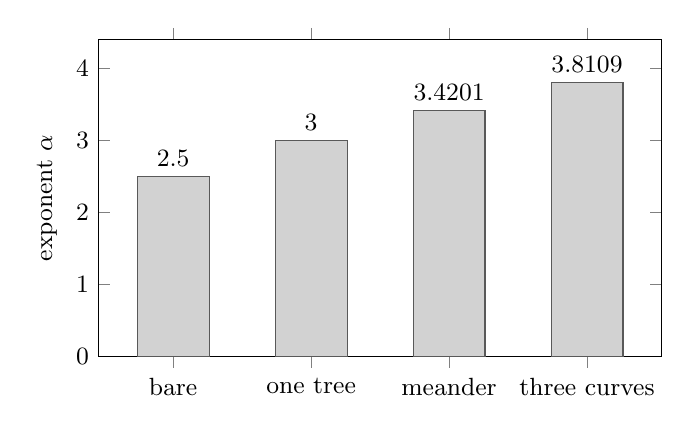
\begin{tikzpicture}
\begin{axis}[ybar,width=0.72\textwidth,height=5.6cm,ymin=0,ymax=4.4,bar width=26pt,
  symbolic x coords={bare,one tree,meander,three curves},xtick=data,
  nodes near coords,nodes near coords style={font=\small},
  every node near coord/.append style={/pgf/number format/fixed,/pgf/number format/precision=4},
  ylabel={exponent $\alpha$},tick label style={font=\small},label style={font=\small},
  enlarge x limits=0.18]
\addplot[fill=gray!35,draw=gray!70!black] coordinates {(bare,2.5) (one tree,3) (meander,3.4201) (three curves,3.8109)};
\end{axis}
\end{tikzpicture}
\caption{The exponent from~\eqref{eq:kpz} for a bare surface ($c=0$), one tree ($c=-2$), two
tree-like curves as in a meander ($c=-4$), and three ($c=-6$). The steps shrink: $+0.5$,
$+0.42$, $+0.39$.}
\label{fig:staircase}
\end{figure}

Figure~\ref{fig:staircase} shows the effect. If the two drawings of a meander simply added their
effects, each would raise the exponent by $1/2$ and meanders would have $\alpha=3.5$. The steps
shrink instead. Intuitively, both drawings live on the same surface, and each additional drawing
has less effect on a surface that the others have already made round.

The first two values of~\eqref{eq:kpz} agree with theorems of Tutte and Mullin. The third, for
meanders, rests on two assumptions that have not been proved for meanders: that each curve
counts as $c=-2$, and that the two curves are independent enough at large scales for their
central charges to add.

\subsection{The exponent and the shape of the surface}\label{sec:shape}

The exponent also has a direct geometric meaning in terms of necks. Take a meander of order $2m$
and draw a vertical line through the middle of the river, between crossings $2m$ and $2m+1$.
Suppose the road meets this line only twice, both times above the river. On the sphere of squares
the line is then a neck that crosses the drawing only twice, and cutting along it and reconnecting
the two road ends on each side produces two meanders of order $m$. Call an arch above the river
\emph{outermost} if no other arch above the river passes over it. The cut-off piece on each side
carries a marked outermost arch, the one created by the reconnection, and conversely two meanders
of order $m$, each with one marked outermost arch, can be glued back in exactly one way. A meander
has at least one outermost arch above the river and, on average, a bounded number of them
(Paper~C). So the number of such meanders lies between $M_m^2$ and a constant times $M_m^2$, and
the chance that a random meander of order $2m$ has this thin neck at its middle is, up to
constant factors,
\[ \frac{M_m^2}{M_{2m}} \;\approx\; \frac{(A\mu^m m^{-\alpha})^2}{A\mu^{2m}(2m)^{-\alpha}} \;=\; A\,2^{\alpha}\, m^{-\alpha} .\]
Here we used the law~\eqref{eq:law}. So $\alpha$ is the exponent of the probability of a thin
neck that cuts the surface into two equal halves. For walks that stay above their start, the same calculation with
Catalan numbers gives $\mathrm{Cat}_m^2/\mathrm{Cat}_{2m}\approx m^{-3/2}$: a walk returns to its starting level at its
midpoint with probability of order $m^{-3/2}$.

\begin{figure}[b]
\centering
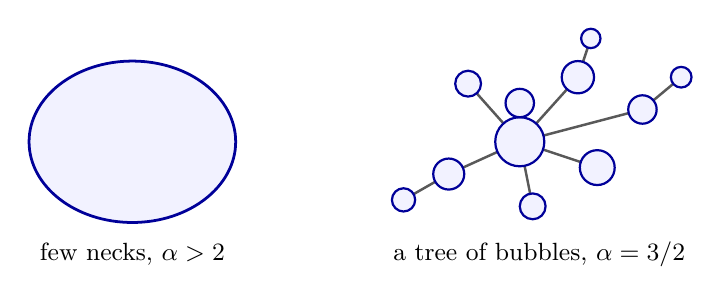
\begin{tikzpicture}[scale=0.82]
  \draw[blue!60!black,line width=1pt,fill=blue!5] (0,0) ellipse (1.6 and 1.25);
  \node[font=\small] at (0,-1.75) {few necks, $\alpha>2$};
  \begin{scope}[xshift=6cm]
  \foreach \a/\b in {0/0.6, 0.9/1.0, -0.8/0.9, 1.2/-0.4, -1.1/-0.5, 0.2/-1.0, 1.9/0.5}
     {\draw[gray!70!black,line width=0.9pt] (0,0)--(\a,\b);}
  \draw[gray!70!black,line width=0.9pt] (1.9,0.5)--(2.5,1.0) (-1.1,-0.5)--(-1.8,-0.9) (0.9,1.0)--(1.1,1.6);
  \foreach \a/\b/\r in {0/0/0.38, 0/0.6/0.22, 0.9/1.0/0.25, -0.8/0.9/0.2, 1.2/-0.4/0.27, -1.1/-0.5/0.24, 0.2/-1.0/0.2, 1.9/0.5/0.22, 2.5/1.0/0.16, -1.8/-0.9/0.18, 1.1/1.6/0.15}
     {\draw[blue!60!black,line width=0.8pt,fill=blue!5] (\a,\b) circle[radius=\r];}
  \node[font=\small] at (0.3,-1.75) {a tree of bubbles, $\alpha=3/2$};
  \end{scope}
\end{tikzpicture}
\caption{Two kinds of large random surface. Left: a round surface in which thin necks are rare.
Right: a surface that has fallen apart into small bubbles joined at necks.}
\label{fig:bubbles}
\end{figure}

Physics gives a picture of two regimes.
\begin{itemize}
\item The KPZ formula~\eqref{eq:kpz} always gives $x\ge1$, so $\alpha\ge2$. As $c$ rises to $1$
it gives $\alpha=2$, and for $c>1$ it has no real solution $x\ge1$. Wherever the formula applies,
balanced necks are rare, and a large random surface is a genuinely two-dimensional blob.
\item When the drawings make necks cheap enough, for instance when many small loops are favored
as in the next paragraph, the formula stops applying. A large random
surface then falls apart into a tree of small bubbles joined at necks
(Figure~\ref{fig:bubbles}), and the exponent is $3/2$, the exponent of trees, because the
bubbles are arranged like the vertices of a random tree.
\end{itemize}
In the physics literature a piece of surface cut off by a neck is called a \emph{baby universe}.

Meanders are predicted to sit in the first regime, but a related family crosses between the two.
A \emph{meandric system} of order $n$ is a pair of arch systems on the same $2n$ crossings, one
above and one below the river, whose arches may form any number of closed loops; meanders are the
systems with one loop. Give each system the weight $q^{k}$, where $q>0$ and $k$ is its number of
loops, and let $Z_n(q)$ be the total weight of the systems of order $n$. For $0\le q\le 2$ the
physical prediction for the exponent of $Z_n(q)$ is again of the form~\eqref{eq:kpz}, with a
central charge that depends on $q$: writing $q=2\cos(\pi\eta)$ with $0\le \eta\le 1/2$,
\[ c(q) \;=\; -1-\frac{6\eta^2}{1-\eta}, \]
which is $-1$ at $q=2$ and $-4$ at $q=0$. The value $q=0$ stands for meanders: as $q\to0$, the
weight divided by $q$ concentrates on the systems with one loop. For large $q$,
systems with many small loops win: the road is broken into many small circles, the surface
becomes a tree of small bubbles held together by the river, and the exponent drops to $3/2$. A
proof of this second regime for $q\ge 167.6$ is in the project repository~\cite{Repo}
(Appendix~\ref{app:repo}); it has not yet been independently checked, and it is not part of
Papers~B--D. Finite-size numerical measurements suggest a crossover, but do not determine the location of a
transition. Beyond $q=2$, the exponent and the onset of the tree regime remain unresolved outside the proved range.

%%%%%%%%%%%%%%%%%%%%%%%%%%%%%%%%%%%%%%%%%%%%%%%%%%%%%%%%%%%%%%%%%%%%%%%%
\section{What is proved for finite meanders}\label{sec:proved}
%%%%%%%%%%%%%%%%%%%%%%%%%%%%%%%%%%%%%%%%%%%%%%%%%%%%%%%%%%%%%%%%%%%%%%%%

For finite meanders the proved statements trap the leftover factor $u_n=M_n/\mu^n$ in a window.
The proofs are in Paper~C~\cite{PaperC}; here we explain why they work.

\begin{theorem}\label{thm:sqrt}
There is a constant $C$ such that for every $n\ge1$
\[ \mu^n e^{-C\sqrt n} \;\le\; M_n \;\le\; \frac{\mu^{n+1}}{8n} . \]
\end{theorem}

The upper bound decays like $n^{-1}$, already a power law but with exponent $1$ instead of
$3.42$. The lower bound decays faster than any power of $n$. So the true $u_n$, believed to be
$A\,n^{-3.4201}$, is proved to lie between $e^{-C\sqrt n}$ and $\mu/(8n)$. In logarithmic terms,
\[ -C\sqrt n \;\le\; \log u_n \;\le\; -\log n + \log(\mu/8),\]
while the prediction is $-3.4201\log n+\log A$. Both bounds are new as far as we know. The
lower bound improves one obtained earlier in this project, which had $C\sqrt n\log n$ in the
exponent. Both sides have a short explanation.

\subsection{The upper bound}\label{sec:upperA}

Meanders can be glued: two meanders of orders $a$ and $b$ can be placed side by side on the
river and their roads joined into one, so that the two pieces can be recovered from the result
(Paper~C). This gives $M_{a+b}\ge M_aM_b$. Fekete's lemma says that a sequence $(y_k)$ with
$y_{j+k}\ge y_j+y_k$ has $y_k/k\to\sup_k y_k/k$. Applied to $y_k=\log M_k$, it shows that
$\mu=\lim M_n^{1/n}$ exists, equals $\sup_n M_n^{1/n}$, and so $M_n\le\mu^n$ for every $n$.

A more careful gluing inserts a second meander of order $n$, capped by one extra pair of
crossings (one on each side of it, joined by a new arch below the river), into a gap of a first
meander of order $n$. The result has order $2n+1$, and the insertion can be done in at least
$4n-1$ ways, all of which can be told apart afterwards. So $M_{2n+1}\ge(4n-1)M_n^2$ (Paper~C), and
since $8(2n+1)(4n-1)\ge64n^2$, the numbers $g(n)=8n\,M_n$ satisfy $g(2n+1)\ge g(n)^2$. The upper
bound follows in two lines. Since $(2n+1)+1=2(n+1)$, the numbers $f(n)=\log g(n)/(n+1)$ satisfy
$f(2n+1)\ge f(n)$.
Iterating along $n,\,2n+1,\,4n+3,\ldots$ gives an increasing sequence whose limit is $\log\mu$,
because $g(n)^{1/n}\to\mu$. So $f(n)\le\log\mu$, that is $8nM_n\le\mu^{n+1}$. Intuitively, if
two halves can be glued in about $n$ ways, a meander of order $2n$ is about $n$ times more common
than a pair of halves, and that forces a factor $1/n$.

\subsection{The lower bound}

The lower bound needs the opposite inequality: a large meander must not be much more common than
a pair of smaller ones. Cut it in two. Let the meander have order $m$, so that its sphere has
$2m$ squares. By a form of the planar separator theorem (balanced separators of this size are
classical for planar graphs~\cite{LT,Miller}), the sphere has a closed curve, a
\emph{separator}, that crosses the river and the road at about $\sqrt m$ points in total and
splits the sphere into two pieces of comparable size. Each piece can be completed to a meander:
draw a new closed curve just outside the piece, made of bits of river and road, and then join the
remaining loose ends outside it so that the river and the road each close up into one curve. The
original meander can be recovered from the two completed ones plus a small record. The new
ingredient is that the number of possible records is at most $e^{Bs}$ for a constant $B$, where
$s$ is the number of points where the separator crosses the drawing. Intuitively, the new curve
can be traced again in the completed meander one step at a time, with at most three choices per
step, so the piece is easy to find. Earlier completions had no such curve and needed about
$m^{s}$ records, which produced the extra logarithm.

With $s$ of order $\sqrt m$ this gives
\[ M_m \;\le\; e^{B'\sqrt m}\, M_a M_b \]
for some $a$ and $b$ that each lie between $m/10$ and $9m/10$ and add up to $m$ plus at most a
constant times $\sqrt m$. In terms of $L(n)=n\log\mu-\log M_n=-\log u_n$, which satisfies
$L(n)\ge0$ and $L(n)/n\to0$, this says $L(a)+L(b)\le L(m)+B''\sqrt m$, so one of the two pieces, of size $k$, has
$L(k)/k\le L(m)/m+B''/\sqrt m$. Start from a huge size and keep passing to such a piece until the
size first drops below a target $n$. The sizes shrink geometrically, so the added terms
$B''/\sqrt{\text{size}}$ sum to at most a constant times $1/\sqrt n$, and the starting term
$L(m)/m$ is as small as we like. This gives some $k$ between $n/10$ and $n$ with
$L(k)\le B'''\sqrt n$. Finally, $L(a+b)\le L(a)+L(b)$, so splitting any $n$ into such blocks of
geometrically decreasing sizes gives $L(n)\le C\sqrt n$, which is Theorem~\ref{thm:sqrt}.

The square root has a clear source. Some planar maps, such as square grids, really need
separators with about $\sqrt m$ crossings, and the argument uses one separator for every meander.
To do better, the separator would have to be shorter, which can only hold for a fraction of
meanders, and that fraction would have to be estimated. Paper~C states exactly what such an
estimate would give. It also gives a second criterion, in terms of meanders whose arches are
nested only to a bounded depth, and shows why building such meanders by gluing short ones cannot
meet it. These criteria are proved but not yet independently checked.

\subsection{Prime meanders}

Say that a meander has a \emph{cut} at the gap between crossings $2m$ and $2m+1$ if no arch
below the river passes over the gap, the crossings $2m$ and $2m+1$ are joined by a short arch
above the river, and exactly one other arch above the river passes over the gap. This is a thin
neck of the kind in Section~\ref{sec:shape}, at any position, and the meanders with a cut are
exactly the pairs glued side by side as at the start of Section~\ref{sec:upperA}. A meander is
\emph{prime} if it has no cut. Every meander factors uniquely into prime meanders (a close
relative of known decompositions), and on average a meander has a bounded number of cuts. A small new result is that the chance of a cut at a given
position tends to zero as the distance of that position from both ends grows; its proof has not
yet been independently checked. These facts, an exact identity that relates the power law to
necks at the middle (used in Section~\ref{sec:bridge}), and exact data are in Paper~C.

%%%%%%%%%%%%%%%%%%%%%%%%%%%%%%%%%%%%%%%%%%%%%%%%%%%%%%%%%%%%%%%%%%%%%%%%
\section{A continuum model in which the KPZ formula is a theorem}\label{sec:continuum}
%%%%%%%%%%%%%%%%%%%%%%%%%%%%%%%%%%%%%%%%%%%%%%%%%%%%%%%%%%%%%%%%%%%%%%%%

The physical argument of Section~\ref{sec:surfaces} has two unproved steps for meanders: that
each curve acts like a spanning tree, and that the effects add up through the central charge.
This section describes a continuum model of random surfaces in which the second step is exact,
and explains the remaining ingredient, which Paper~D proves. In this section $N$ denotes a number
of squares, not the order of a meander.

\subsection{From counting to a continuum}\label{sec:dictionary}

The rest of the paper speaks the language of continuum random surfaces. This subsection explains
how that language translates the counting of Sections~\ref{sec:walks} and~\ref{sec:surfaces},
in three steps, and Table~\ref{tab:dictionary} collects the translation.

\emph{Step 1: describe a large surface by where its area sits.} Any sphere of squares can be
spread out over a round sphere in an essentially unique way that preserves angles (by the
uniformization theorem of complex analysis), much as a map of the Earth spreads the globe over a
flat page. After this, the surface is recorded by a single function on the round sphere: how
densely its squares are packed near each point. Write this density as $e^{\gamma h}$, where $h$
is a random function and $\gamma$ a number that sets how strongly $h$ is felt. For a uniformly
random sphere of squares, the logarithm of the density is predicted to be a \emph{Gaussian free
field}, the two-dimensional analog of Brownian motion described below. Intuitively, Brownian
motion records the ups and downs of a random walk, and the Gaussian free field records where a
random surface is crowded and where it is sparse.

\emph{Step 2: drawings change the law of the field.} Counting surfaces together with drawings
multiplies the weight of each surface by its number of drawings, which by~\eqref{eq:charge} is a
power of $\det\Delta_G$ up to a size factor. A classical formula of Polyakov says how this
determinant depends on the shape: its logarithm is a constant times the \emph{energy}
$\int|\nabla h|^2$ of the field, plus simpler terms that shift the field or depend only on the
size, without changing how much the field fluctuates. The weight of a Gaussian
field is itself of the form $e^{-\text{const}\cdot\int|\nabla h|^2}$. Multiplying one Gaussian
weight by another gives a Gaussian weight again, with a changed constant. So a drawing does not
change the kind of random surface; it only changes the parameter $\gamma$. Each spanning tree
changes it by the same amount, which is the additivity of $c$ in continuum form. Trees make the
field smoother, so $\gamma$ decreases: $\gamma^2=8/3$ for bare surfaces, $2$ with one tree, and
$(17-\sqrt{145})/3\approx1.653$ with two.

\emph{Step 3: read off the exponent from the size.} A counting law $\mu^n n^{-\alpha}$ becomes
a statement about the size of the surface: the total weight of surfaces of size at least $n$
decays like $n^{-(\alpha-1)}$ (Section~\ref{sec:surfaces}). In the continuum the size is a random
variable, and the question becomes how heavy its tail is. The growth rate $\mu$ has no continuum
counterpart: it counts local choices, and those are invisible after zooming out.

\begin{table}[ht]
\centering
\small
\renewcommand{\arraystretch}{1.15}
\begin{tabular}{p{0.47\textwidth}p{0.43\textwidth}}
\toprule
counting & continuum \\
\midrule
number of squares & area, or the number of squares of a random subdivision \\
uniformly random sphere of squares, $c=0$ & field with $\gamma^2=8/3$ (the Brownian map) \\
each sphere counted with its spanning trees, $c=-2$ & field with $\gamma^2=2$ \\
two tree-like drawings (a meander), $c=-4$ & field with $\gamma^2=(17-\sqrt{145})/3$ \\
a curve visiting every square once & a random curve through every point (SLE$_8$, Section~\ref{sec:limit}) \\
counting exponent $\alpha$ & one plus the tail exponent of the size, $1+4/\gamma^2$ \\
growth rate $\mu$ & no counterpart (a local quantity) \\
thin neck splitting a meander into halves & near-split of the two curves (Section~\ref{sec:limit}) \\
\bottomrule
\end{tabular}
\caption{A dictionary between counting and the continuum. Each entry on the right is a model or a
prediction, not a theorem about the entry on the left; the next subsections say which parts are
proved.}
\label{tab:dictionary}
\end{table}

The model below makes Steps~2 and~3 exact for a continuum surface built directly from a Gaussian
free field, with squares in place of area.

\subsection{Random surfaces from a random field}

The model is built from the \emph{Gaussian free field} $h$ on the sphere. It is a random
function whose values $h(z)$ and $h(w)$ at two points have covariance about $-\log|z-w|$, minus
the logarithm of their distance. It is too rough to have values at single points, since this
covariance is infinite at $z=w$, but its average $h_S$ over a square
$S$ is an ordinary normal random variable, with variance about $\log(1/|S|)$, where $|S|$ denotes
the side length of $S$. Intuitively, $h$ is the two-dimensional analog of Brownian motion. We use
it on a fixed unit square drawn on the sphere.

Fix a parameter $Q\ge2$ and a small number $\varepsilon>0$. Start from the unit square and repeat
the following rule: split a square $S$ into four equal squares if
\[ e^{h_S/Q}\,|S| \;>\; \varepsilon ,\]
and keep it otherwise. Let $N$ be the number of squares at the end. Intuitively,
$e^{h_S/Q}|S|$ is the size of $S$ as seen by the field. Where the field is high, squares count as
large and are split again and again, so high regions are covered by many small squares. Intuitively, the final squares play the role of the faces of a random planar map, and
$N$ is the size of the surface. The parameter $Q$ enters only through this rule; the field itself
does not depend on it. This construction is due to Ang, Park, Pfeffer and
Sheffield~\cite{APPS}, following earlier work on the same subdivisions~\cite{DS}.

The parameter $Q$ is tied to the central charge $c$ by $Q^2=(25-c)/6$, so $Q\ge2$ corresponds to
$c\le1$. This is how the physics literature matches $Q$ to $c$, and the next subsection shows why it
is natural: adding $k$ spanning trees raises $Q^2$ by $k/3$, which is exactly a drop of $2k$ in
$c$. The probability literature usually writes $Q$ through a second number $\gamma\in(0,2]$,
\begin{equation}\label{eq:Q}
Q^2 \;=\; \frac{25-c}{6}, \qquad Q \;=\; \frac{2}{\gamma}+\frac{\gamma}{2};
\end{equation}
of the two solutions $\gamma$ of the second equation we take the one in $(0,2]$. So $\gamma=2$ at
$Q=2$, and $\gamma\to0$ as $Q\to\infty$. A bare surface, $c=0$, has $Q^2=25/6$ and
$\gamma^2=8/3$; the meander value $c=-4$ has $Q^2=29/6$ and
$\gamma^2=(17-\sqrt{145})/3\approx1.653$. Squaring the second relation gives
$Q^2-2=4/\gamma^2+\gamma^2/4$, so with $x=4/\gamma^2$ it says exactly $x+1/x=(13-c)/6$. The KPZ
formula~\eqref{eq:kpz} is therefore the statement that the tail exponent $x$ equals $4/\gamma^2$.

\subsection{Drawings as an exact change of parameter}

For a planar map, the number of spanning trees equals a determinant built from the map's
Laplacian matrix, by Kirchhoff's theorem; equivalently, it is the product of the nonzero
eigenvalues of the Laplacian, divided by the number of vertices. The continuum model has an
analog. The Laplacian of a
continuum surface has infinitely many eigenvalues, so their product has to be renormalized; the
result is the \emph{regularized determinant}. Ang, Park, Pfeffer and Sheffield proved that
weighting the model by the $k$-th power of this determinant has exactly the same effect, for
surfaces with a given number of squares, as changing $Q^2$ to $Q^2+k/3$, that is, $c$ to
$c-2k$~\cite[Theorem~6.9]{APPS}. Intuitively, in this model drawing $k$ spanning trees is the
same as lowering the central charge by $2k$. The additivity of $c$, which is an assumption for
meanders, is here a theorem.

Write $Q_k$ for the parameter after the change, $Q_k^2=Q^2+k/3$. Their theorem compares
surfaces with the same number of squares. Comparing surfaces with different numbers of squares
needs two corrections, which Paper~D derives. The determinant contains a factor proportional to
$N^{1/3}$, which must be divided out. And the comparison of the two models is a Gaussian change of
variables, which contributes a factor $Q/Q_k$ for each square, so $(Q/Q_k)^N$ in all; one
multiplies by its inverse. This second factor is purely exponential in $N$: like $\mu^n$ for
meanders, it changes the growth rate but not the exponent.

\subsection{The tail law}

What was missing to read off an exponent is the distribution of the number of squares. It is
proved in Paper~D~\cite{PaperD}.

\begin{theorem}[Paper~D~\cite{PaperD}]\label{thm:tail}
For every $Q\ge2$ and every fixed $\varepsilon>0$,
\[ \lim_{n\to\infty}\frac{\log \Pr(N\ge n)}{\log n} \;=\; -\frac{4}{\gamma^2}, \]
with $\gamma$ given by~\eqref{eq:Q}.
\end{theorem}

Combined with the exact change of parameter, this gives the full KPZ curve.

\begin{theorem}[Paper~D~\cite{PaperD}]\label{thm:apps}
In the model above at $c=0$, with $Q_0^2=25/6$, weight each surface by the $k$-th power of the
regularized determinant, divided by $N^{k/3}$, and by the factor $(Q_k/Q_0)^N$ with
$Q_k^2=Q_0^2+k/3$. For every real $k\ge-1/2$, the total weight of surfaces with at least $n$
squares is $n^{-x_k+o(1)}$, where
\[ x_k+\frac1{x_k} \;=\; \frac{13+2k}{6},\qquad x_k\ge1 .\]
At $k=2$, the analog of two spanning trees, $x_2=(17+\sqrt{145})/12$, so
$1+x_2=\alpha_*$.
\end{theorem}

By the discussion after~\eqref{eq:kpz}, a tail exponent $x_2$ corresponds to the counting
exponent $1+x_2$. Two caveats keep this in proportion. The statement is about cumulative tails,
$\Pr(N\ge n)$, up to factors $n^{o(1)}$, not about the probability of each size. And it concerns
a continuum model in which the spanning trees are replaced by a determinant; it says nothing
directly about meanders, where the curves are actual curves on a discrete surface.

\subsection{Idea of the proof}\label{sec:tailidea}

We describe the upper bound for $Q>2$; the endpoint $Q=2$ needs a separate argument, given in
Paper~D. The number of squares is large only if the field is unusually high somewhere, since
high regions are where squares keep splitting. Count the squares of side $2^{-j}$ whose split
condition holds.
For a number $a>0$, the condition $e^{h_S/Q}2^{-j}>\varepsilon$ implies
$(e^{h_S/Q}2^{-j}/\varepsilon)^{aQ}>1$, and averaging over the $4^j$ squares at that depth shows
that their number is at most a constant times
\[ 2^{\,j\,(2-aQ+a^2/2)} \]
times a random factor whose $p$-th moment, the expected value of its $p$-th power, is finite for
every $p<4/a^2$. The exponent
$2-aQ+a^2/2$ is a quadratic in $a$ whose two roots are $\gamma$ and $4/\gamma$, as one checks from
$Q=2/\gamma+\gamma/2$. It is negative exactly between them. Choosing $a$ slightly above $\gamma$
makes the counts summable over $j$ and shows that the $p$-th moment of $N$ is finite for every
$p<4/\gamma^2$. By Markov's inequality, $\Pr(N\ge n)\le \mathbb E[N^p]\,n^{-p}$ for each such
order $p$, hence $\Pr(N\ge n)\le n^{-4/\gamma^2+o(1)}$. The matching lower bound comes from the
cheapest way to make $N$ large: raise the field over one small square, which happens with a
probability of the predicted size, and show that its descendants then produce enough squares.

The ratio of the two roots, $(4/\gamma)/\gamma=4/\gamma^2$, is exactly the KPZ number $x$. This
is where the quadratic of the physical prediction comes from in the proof.

\subsection{Area versus number of squares}\label{sec:area}

The surface also carries an area: the integral of $e^{\gamma h}$, suitably renormalized because
$h$ has no values at points. A square of side $|S|$ has area roughly $e^{\gamma h_S}|S|^{\gamma Q}$,
and the splitting rule $e^{h_S/Q}|S|>\varepsilon$ is the same as asking that this rough area
exceed $\varepsilon^{\gamma Q}$. So the rule splits squares until each has small area. A natural
first idea is that $N$ should be proportional to the area, whose tail is
known~\cite{RV,Wong}. For $Q>2$ this is false in a precise sense (Paper~D): given that the area is
very large, the probability that $N=1$ stays bounded away from zero. The field can be very high on
fine scales inside a square that the splitting rule never inspects, because the rule only looks
at averages over squares it has already created. The proof of Theorem~\ref{thm:tail} therefore
works with the squares directly.

\subsection{A branching random walk model}\label{sec:cascade}

A simpler model shows the mechanism in its purest form. Call
$H(S)=h_S+Q\log(|S|/\varepsilon)$ the \emph{height} of a square, so that $S$ is split exactly when
$H(S)>0$. Passing from a square to one of its four children lowers $Q\log|S|$ by $Q\log2$ and
changes $h_S$ by a random amount of variance about $\log2$. In the toy model these random amounts
are independent normal steps, independent for different children; in the model of
Section~\ref{sec:continuum} they are correlated. A square is split while its height is positive.
The squares then form a \emph{branching random walk killed at zero}: each square has four
children, each child's height is its parent's height plus a random step, and a square whose height
is not positive has no children. The number $N$ of final squares is determined by this family
tree, and for $Q>2$ its tail is known precisely~\cite{AHZ}:
\[ \Pr(N\ge n) \;\sim\; \mathrm{const}\cdot n^{-x}, \qquad x \;=\; \frac{\lambda_+}{\lambda_-},
\qquad \lambda_\pm \;=\; Q\pm\sqrt{Q^2-4}. \]
The two rates are the roots of Section~\ref{sec:tailidea}: $\lambda_-=\gamma$ and
$\lambda_+=4/\gamma$. Since $\lambda_+\lambda_-=4$ and $\lambda_++\lambda_-=2Q$,
\[ x+\frac1x \;=\; \frac{\lambda_+^2+\lambda_-^2}{\lambda_+\lambda_-} \;=\; Q^2-2 \;=\; \frac{13-c}{6} .\]
So the KPZ quadratic is the relation between the two exponential rates of a killed branching
random walk. In this toy model Paper~D also proves the local version: for $Q>2$, every
starting height and every $n$ that is one more than a multiple of $3$ (the only possible values,
since each split adds three squares), $\Pr(N=n)$ lies between two constant multiples of
$n^{-1-x}$. At $Q^2=29/6$ the
exponent $1+x$ is again $\alpha_*$.

%%%%%%%%%%%%%%%%%%%%%%%%%%%%%%%%%%%%%%%%%%%%%%%%%%%%%%%%%%%%%%%%%%%%%%%%
\section{The conjectured limit of large meanders}\label{sec:limit}
%%%%%%%%%%%%%%%%%%%%%%%%%%%%%%%%%%%%%%%%%%%%%%%%%%%%%%%%%%%%%%%%%%%%%%%%

\subsection{The conjecture}

Borga, Gwynne and Sun proposed a precise description of what a large uniformly random meander
looks like when zoomed out~\cite{BGS}. It has four ingredients.

\begin{itemize}
\item \emph{The surface} is a \emph{Liouville quantum gravity sphere} (the name comes from
physics): a continuum random surface of total area one, built from the Gaussian free field as in
Section~\ref{sec:continuum}, with the size of a region measured by the area $\int e^{\gamma h}$ of
Section~\ref{sec:area} instead of by counting squares. Its parameter is
$\gamma^2=(17-\sqrt{145})/3$, the value that~\eqref{eq:Q} assigns to $c=-4$.
\item \emph{The river and the road} become two random curves. Recall that each of them visits
every square of the sphere exactly once. When the squares become infinitely small, such a curve
becomes a continuous curve that passes through every point of the surface, like the
space-filling curves of Peano and Hilbert, but random. Which random curve it is, is known for
spanning trees (Figure~\ref{fig:peano}). Walk around a spanning tree of a fine grid, keeping the
tree on your left. This path visits the neighborhood of every vertex and returns to its start,
and as the grid gets finer it converges to a particular random space-filling curve, called
SLE$_8$~\cite{LSWust}. (SLE, for Schramm--Loewner evolution, is a family of random curves indexed
by a number; the value $8$ gives the curve that fills space.) Since the river and the road are
expected to behave like spanning trees (Section~\ref{sec:charge}), both become SLE$_8$ curves.
\item \emph{The two curves are independent} of each other and of the surface. Intuitively,
zoomed out, knowing the river tells nothing about the road. This is the continuum form of the
assumption that the two central charges add.
\item \emph{Time along each curve is measured by area}: by time $t$ the curve has covered area $t$,
and it covers the whole surface by time one. This is the continuum version of numbering the
crossings: the $i$-th crossing along the river corresponds to time about $i/(2n)$ along the
river curve, and similarly for the road.
\end{itemize}

\begin{figure}[ht]
\centering
% Path around a random spanning tree (Wilsons algorithm); generated by a script.
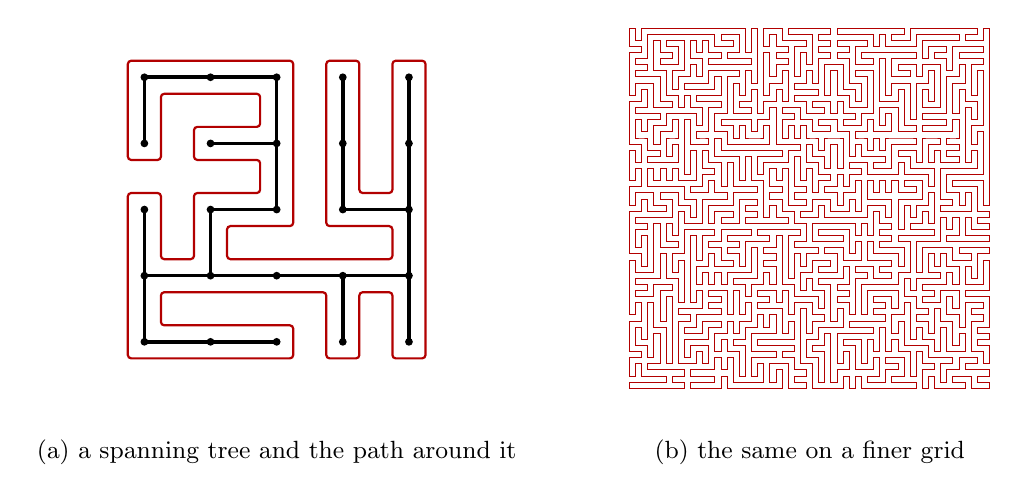
\begin{tikzpicture}
\begin{scope}[x=0.420cm,y=0.420cm,yshift=0.55cm]
  \draw[red!70!black,line width=0.8pt,rounded corners=1.2pt] (3.5,-0.5) -- (4.5,-0.5) -- (4.5,0.5) -- (3.5,0.5) -- (2.5,0.5) -- (1.5,0.5) -- (0.5,0.5) -- (0.5,1.5) -- (1.5,1.5) -- (2.5,1.5) -- (3.5,1.5) -- (4.5,1.5) -- (5.5,1.5) -- (5.5,0.5) -- (5.5,-0.5) -- (6.5,-0.5) -- (6.5,0.5) -- (6.5,1.5) -- (7.5,1.5) -- (7.5,0.5) -- (7.5,-0.5) -- (8.5,-0.5) -- (8.5,0.5) -- (8.5,1.5) -- (8.5,2.5) -- (8.5,3.5) -- (8.5,4.5) -- (8.5,5.5) -- (8.5,6.5) -- (8.5,7.5) -- (8.5,8.5) -- (7.5,8.5) -- (7.5,7.5) -- (7.5,6.5) -- (7.5,5.5) -- (7.5,4.5) -- (6.5,4.5) -- (6.5,5.5) -- (6.5,6.5) -- (6.5,7.5) -- (6.5,8.5) -- (5.5,8.5) -- (5.5,7.5) -- (5.5,6.5) -- (5.5,5.5) -- (5.5,4.5) -- (5.5,3.5) -- (6.5,3.5) -- (7.5,3.5) -- (7.5,2.5) -- (6.5,2.5) -- (5.5,2.5) -- (4.5,2.5) -- (3.5,2.5) -- (2.5,2.5) -- (2.5,3.5) -- (3.5,3.5) -- (4.5,3.5) -- (4.5,4.5) -- (4.5,5.5) -- (4.5,6.5) -- (4.5,7.5) -- (4.5,8.5) -- (3.5,8.5) -- (2.5,8.5) -- (1.5,8.5) -- (0.5,8.5) -- (-0.5,8.5) -- (-0.5,7.5) -- (-0.5,6.5) -- (-0.5,5.5) -- (0.5,5.5) -- (0.5,6.5) -- (0.5,7.5) -- (1.5,7.5) -- (2.5,7.5) -- (3.5,7.5) -- (3.5,6.5) -- (2.5,6.5) -- (1.5,6.5) -- (1.5,5.5) -- (2.5,5.5) -- (3.5,5.5) -- (3.5,4.5) -- (2.5,4.5) -- (1.5,4.5) -- (1.5,3.5) -- (1.5,2.5) -- (0.5,2.5) -- (0.5,3.5) -- (0.5,4.5) -- (-0.5,4.5) -- (-0.5,3.5) -- (-0.5,2.5) -- (-0.5,1.5) -- (-0.5,0.5) -- (-0.5,-0.5) -- (0.5,-0.5) -- (1.5,-0.5) -- (2.5,-0.5) -- cycle;
  \draw[line width=1.3pt] (0,2)--(0,0);
  \draw[line width=1.3pt] (0,4)--(0,2);
  \draw[line width=1.3pt] (0,6)--(0,8);
  \draw[line width=1.3pt] (0,8)--(2,8);
  \draw[line width=1.3pt] (2,8)--(4,8);
  \draw[line width=1.3pt] (4,8)--(4,6);
  \draw[line width=1.3pt] (4,6)--(4,4);
  \draw[line width=1.3pt] (4,4)--(2,4);
  \draw[line width=1.3pt] (2,4)--(2,2);
  \draw[line width=1.3pt] (2,2)--(0,2);
  \draw[line width=1.3pt] (2,0)--(0,0);
  \draw[line width=1.3pt] (2,6)--(4,6);
  \draw[line width=1.3pt] (4,0)--(2,0);
  \draw[line width=1.3pt] (4,2)--(2,2);
  \draw[line width=1.3pt] (6,0)--(6,2);
  \draw[line width=1.3pt] (6,2)--(4,2);
  \draw[line width=1.3pt] (6,4)--(8,4);
  \draw[line width=1.3pt] (8,4)--(8,2);
  \draw[line width=1.3pt] (8,2)--(6,2);
  \draw[line width=1.3pt] (6,6)--(6,4);
  \draw[line width=1.3pt] (6,8)--(6,6);
  \draw[line width=1.3pt] (8,0)--(8,2);
  \draw[line width=1.3pt] (8,6)--(8,4);
  \draw[line width=1.3pt] (8,8)--(8,6);
  \foreach \i in {0,...,4} \foreach \j in {0,...,4} \fill (2*\i,2*\j) circle[radius=1.4pt];
\end{scope}
\begin{scope}[xshift=6.2cm]
\begin{scope}[x=0.0775cm,y=0.0775cm]
  \draw[red!70!black,line width=0.35pt] (26.5,20.5) -- (26.5,21.5) -- (27.5,21.5) -- (27.5,20.5) -- (27.5,19.5) -- (28.5,19.5) -- (28.5,20.5) -- (28.5,21.5) -- (29.5,21.5) -- (30.5,21.5) -- (30.5,22.5) -- (29.5,22.5) -- (28.5,22.5) -- (27.5,22.5) -- (26.5,22.5) -- (26.5,23.5) -- (27.5,23.5) -- (28.5,23.5) -- (28.5,24.5) -- (28.5,25.5) -- (28.5,26.5) -- (27.5,26.5) -- (26.5,26.5) -- (26.5,27.5) -- (26.5,28.5) -- (25.5,28.5) -- (24.5,28.5) -- (24.5,29.5) -- (24.5,30.5) -- (23.5,30.5) -- (22.5,30.5) -- (22.5,31.5) -- (23.5,31.5) -- (24.5,31.5) -- (24.5,32.5) -- (23.5,32.5) -- (22.5,32.5) -- (22.5,33.5) -- (22.5,34.5) -- (22.5,35.5) -- (23.5,35.5) -- (23.5,34.5) -- (23.5,33.5) -- (24.5,33.5) -- (24.5,34.5) -- (24.5,35.5) -- (25.5,35.5) -- (25.5,34.5) -- (25.5,33.5) -- (25.5,32.5) -- (25.5,31.5) -- (25.5,30.5) -- (25.5,29.5) -- (26.5,29.5) -- (27.5,29.5) -- (28.5,29.5) -- (28.5,30.5) -- (27.5,30.5) -- (26.5,30.5) -- (26.5,31.5) -- (27.5,31.5) -- (28.5,31.5) -- (28.5,32.5) -- (27.5,32.5) -- (26.5,32.5) -- (26.5,33.5) -- (26.5,34.5) -- (26.5,35.5) -- (26.5,36.5) -- (26.5,37.5) -- (27.5,37.5) -- (27.5,36.5) -- (27.5,35.5) -- (27.5,34.5) -- (27.5,33.5) -- (28.5,33.5) -- (28.5,34.5) -- (28.5,35.5) -- (29.5,35.5) -- (29.5,34.5) -- (29.5,33.5) -- (29.5,32.5) -- (29.5,31.5) -- (30.5,31.5) -- (30.5,32.5) -- (30.5,33.5) -- (31.5,33.5) -- (32.5,33.5) -- (32.5,34.5) -- (31.5,34.5) -- (30.5,34.5) -- (30.5,35.5) -- (30.5,36.5) -- (29.5,36.5) -- (28.5,36.5) -- (28.5,37.5) -- (28.5,38.5) -- (28.5,39.5) -- (29.5,39.5) -- (29.5,38.5) -- (29.5,37.5) -- (30.5,37.5) -- (31.5,37.5) -- (31.5,36.5) -- (31.5,35.5) -- (32.5,35.5) -- (32.5,36.5) -- (32.5,37.5) -- (32.5,38.5) -- (32.5,39.5) -- (33.5,39.5) -- (33.5,38.5) -- (33.5,37.5) -- (33.5,36.5) -- (33.5,35.5) -- (34.5,35.5) -- (34.5,36.5) -- (34.5,37.5) -- (34.5,38.5) -- (34.5,39.5) -- (34.5,40.5) -- (33.5,40.5) -- (32.5,40.5) -- (31.5,40.5) -- (31.5,39.5) -- (31.5,38.5) -- (30.5,38.5) -- (30.5,39.5) -- (30.5,40.5) -- (29.5,40.5) -- (28.5,40.5) -- (28.5,41.5) -- (28.5,42.5) -- (27.5,42.5) -- (27.5,41.5) -- (27.5,40.5) -- (26.5,40.5) -- (26.5,41.5) -- (26.5,42.5) -- (25.5,42.5) -- (25.5,41.5) -- (25.5,40.5) -- (24.5,40.5) -- (24.5,41.5) -- (24.5,42.5) -- (24.5,43.5) -- (25.5,43.5) -- (26.5,43.5) -- (26.5,44.5) -- (25.5,44.5) -- (24.5,44.5) -- (24.5,45.5) -- (25.5,45.5) -- (26.5,45.5) -- (27.5,45.5) -- (27.5,44.5) -- (27.5,43.5) -- (28.5,43.5) -- (29.5,43.5) -- (29.5,42.5) -- (29.5,41.5) -- (30.5,41.5) -- (31.5,41.5) -- (32.5,41.5) -- (32.5,42.5) -- (31.5,42.5) -- (30.5,42.5) -- (30.5,43.5) -- (31.5,43.5) -- (32.5,43.5) -- (33.5,43.5) -- (33.5,42.5) -- (33.5,41.5) -- (34.5,41.5) -- (35.5,41.5) -- (35.5,40.5) -- (35.5,39.5) -- (35.5,38.5) -- (35.5,37.5) -- (36.5,37.5) -- (36.5,38.5) -- (36.5,39.5) -- (37.5,39.5) -- (37.5,38.5) -- (37.5,37.5) -- (38.5,37.5) -- (39.5,37.5) -- (40.5,37.5) -- (41.5,37.5) -- (41.5,36.5) -- (40.5,36.5) -- (39.5,36.5) -- (39.5,35.5) -- (40.5,35.5) -- (41.5,35.5) -- (42.5,35.5) -- (42.5,36.5) -- (42.5,37.5) -- (42.5,38.5) -- (42.5,39.5) -- (43.5,39.5) -- (44.5,39.5) -- (45.5,39.5) -- (46.5,39.5) -- (46.5,40.5) -- (45.5,40.5) -- (44.5,40.5) -- (43.5,40.5) -- (42.5,40.5) -- (41.5,40.5) -- (41.5,39.5) -- (41.5,38.5) -- (40.5,38.5) -- (40.5,39.5) -- (40.5,40.5) -- (39.5,40.5) -- (39.5,39.5) -- (39.5,38.5) -- (38.5,38.5) -- (38.5,39.5) -- (38.5,40.5) -- (37.5,40.5) -- (36.5,40.5) -- (36.5,41.5) -- (37.5,41.5) -- (38.5,41.5) -- (38.5,42.5) -- (38.5,43.5) -- (39.5,43.5) -- (39.5,42.5) -- (39.5,41.5) -- (40.5,41.5) -- (41.5,41.5) -- (42.5,41.5) -- (42.5,42.5) -- (42.5,43.5) -- (42.5,44.5) -- (41.5,44.5) -- (41.5,43.5) -- (41.5,42.5) -- (40.5,42.5) -- (40.5,43.5) -- (40.5,44.5) -- (40.5,45.5) -- (41.5,45.5) -- (42.5,45.5) -- (43.5,45.5) -- (43.5,44.5) -- (43.5,43.5) -- (43.5,42.5) -- (43.5,41.5) -- (44.5,41.5) -- (45.5,41.5) -- (46.5,41.5) -- (46.5,42.5) -- (45.5,42.5) -- (44.5,42.5) -- (44.5,43.5) -- (44.5,44.5) -- (44.5,45.5) -- (44.5,46.5) -- (44.5,47.5) -- (44.5,48.5) -- (43.5,48.5) -- (43.5,47.5) -- (43.5,46.5) -- (42.5,46.5) -- (41.5,46.5) -- (40.5,46.5) -- (40.5,47.5) -- (40.5,48.5) -- (40.5,49.5) -- (40.5,50.5) -- (40.5,51.5) -- (40.5,52.5) -- (40.5,53.5) -- (41.5,53.5) -- (41.5,52.5) -- (41.5,51.5) -- (41.5,50.5) -- (41.5,49.5) -- (41.5,48.5) -- (41.5,47.5) -- (42.5,47.5) -- (42.5,48.5) -- (42.5,49.5) -- (43.5,49.5) -- (44.5,49.5) -- (45.5,49.5) -- (45.5,48.5) -- (45.5,47.5) -- (45.5,46.5) -- (45.5,45.5) -- (45.5,44.5) -- (45.5,43.5) -- (46.5,43.5) -- (46.5,44.5) -- (46.5,45.5) -- (46.5,46.5) -- (46.5,47.5) -- (46.5,48.5) -- (46.5,49.5) -- (47.5,49.5) -- (48.5,49.5) -- (48.5,50.5) -- (48.5,51.5) -- (49.5,51.5) -- (49.5,50.5) -- (49.5,49.5) -- (49.5,48.5) -- (49.5,47.5) -- (49.5,46.5) -- (48.5,46.5) -- (48.5,47.5) -- (48.5,48.5) -- (47.5,48.5) -- (47.5,47.5) -- (47.5,46.5) -- (47.5,45.5) -- (48.5,45.5) -- (49.5,45.5) -- (50.5,45.5) -- (50.5,46.5) -- (50.5,47.5) -- (50.5,48.5) -- (50.5,49.5) -- (50.5,50.5) -- (50.5,51.5) -- (50.5,52.5) -- (49.5,52.5) -- (48.5,52.5) -- (47.5,52.5) -- (47.5,51.5) -- (47.5,50.5) -- (46.5,50.5) -- (46.5,51.5) -- (46.5,52.5) -- (45.5,52.5) -- (44.5,52.5) -- (43.5,52.5) -- (43.5,51.5) -- (44.5,51.5) -- (45.5,51.5) -- (45.5,50.5) -- (44.5,50.5) -- (43.5,50.5) -- (42.5,50.5) -- (42.5,51.5) -- (42.5,52.5) -- (42.5,53.5) -- (43.5,53.5) -- (44.5,53.5) -- (45.5,53.5) -- (46.5,53.5) -- (46.5,54.5) -- (45.5,54.5) -- (44.5,54.5) -- (43.5,54.5) -- (42.5,54.5) -- (41.5,54.5) -- (40.5,54.5) -- (39.5,54.5) -- (38.5,54.5) -- (37.5,54.5) -- (37.5,53.5) -- (38.5,53.5) -- (39.5,53.5) -- (39.5,52.5) -- (38.5,52.5) -- (37.5,52.5) -- (36.5,52.5) -- (36.5,53.5) -- (36.5,54.5) -- (36.5,55.5) -- (37.5,55.5) -- (38.5,55.5) -- (38.5,56.5) -- (37.5,56.5) -- (36.5,56.5) -- (35.5,56.5) -- (34.5,56.5) -- (33.5,56.5) -- (33.5,55.5) -- (34.5,55.5) -- (35.5,55.5) -- (35.5,54.5) -- (34.5,54.5) -- (33.5,54.5) -- (33.5,53.5) -- (34.5,53.5) -- (35.5,53.5) -- (35.5,52.5) -- (35.5,51.5) -- (35.5,50.5) -- (35.5,49.5) -- (36.5,49.5) -- (37.5,49.5) -- (37.5,48.5) -- (37.5,47.5) -- (37.5,46.5) -- (36.5,46.5) -- (36.5,47.5) -- (36.5,48.5) -- (35.5,48.5) -- (34.5,48.5) -- (34.5,49.5) -- (34.5,50.5) -- (34.5,51.5) -- (34.5,52.5) -- (33.5,52.5) -- (32.5,52.5) -- (31.5,52.5) -- (31.5,51.5) -- (31.5,50.5) -- (31.5,49.5) -- (31.5,48.5) -- (31.5,47.5) -- (32.5,47.5) -- (32.5,48.5) -- (32.5,49.5) -- (32.5,50.5) -- (32.5,51.5) -- (33.5,51.5) -- (33.5,50.5) -- (33.5,49.5) -- (33.5,48.5) -- (33.5,47.5) -- (34.5,47.5) -- (35.5,47.5) -- (35.5,46.5) -- (35.5,45.5) -- (36.5,45.5) -- (37.5,45.5) -- (38.5,45.5) -- (38.5,46.5) -- (38.5,47.5) -- (38.5,48.5) -- (38.5,49.5) -- (38.5,50.5) -- (37.5,50.5) -- (36.5,50.5) -- (36.5,51.5) -- (37.5,51.5) -- (38.5,51.5) -- (39.5,51.5) -- (39.5,50.5) -- (39.5,49.5) -- (39.5,48.5) -- (39.5,47.5) -- (39.5,46.5) -- (39.5,45.5) -- (39.5,44.5) -- (38.5,44.5) -- (37.5,44.5) -- (37.5,43.5) -- (37.5,42.5) -- (36.5,42.5) -- (35.5,42.5) -- (34.5,42.5) -- (34.5,43.5) -- (35.5,43.5) -- (36.5,43.5) -- (36.5,44.5) -- (35.5,44.5) -- (34.5,44.5) -- (34.5,45.5) -- (34.5,46.5) -- (33.5,46.5) -- (33.5,45.5) -- (33.5,44.5) -- (32.5,44.5) -- (32.5,45.5) -- (32.5,46.5) -- (31.5,46.5) -- (30.5,46.5) -- (29.5,46.5) -- (29.5,45.5) -- (30.5,45.5) -- (31.5,45.5) -- (31.5,44.5) -- (30.5,44.5) -- (29.5,44.5) -- (28.5,44.5) -- (28.5,45.5) -- (28.5,46.5) -- (27.5,46.5) -- (26.5,46.5) -- (26.5,47.5) -- (27.5,47.5) -- (28.5,47.5) -- (29.5,47.5) -- (30.5,47.5) -- (30.5,48.5) -- (29.5,48.5) -- (28.5,48.5) -- (27.5,48.5) -- (26.5,48.5) -- (26.5,49.5) -- (27.5,49.5) -- (28.5,49.5) -- (28.5,50.5) -- (28.5,51.5) -- (29.5,51.5) -- (29.5,50.5) -- (29.5,49.5) -- (30.5,49.5) -- (30.5,50.5) -- (30.5,51.5) -- (30.5,52.5) -- (30.5,53.5) -- (31.5,53.5) -- (32.5,53.5) -- (32.5,54.5) -- (31.5,54.5) -- (30.5,54.5) -- (30.5,55.5) -- (31.5,55.5) -- (32.5,55.5) -- (32.5,56.5) -- (31.5,56.5) -- (30.5,56.5) -- (30.5,57.5) -- (31.5,57.5) -- (32.5,57.5) -- (32.5,58.5) -- (31.5,58.5) -- (30.5,58.5) -- (29.5,58.5) -- (28.5,58.5) -- (27.5,58.5) -- (26.5,58.5) -- (25.5,58.5) -- (25.5,57.5) -- (26.5,57.5) -- (27.5,57.5) -- (28.5,57.5) -- (29.5,57.5) -- (29.5,56.5) -- (29.5,55.5) -- (29.5,54.5) -- (29.5,53.5) -- (29.5,52.5) -- (28.5,52.5) -- (28.5,53.5) -- (28.5,54.5) -- (27.5,54.5) -- (27.5,53.5) -- (27.5,52.5) -- (27.5,51.5) -- (27.5,50.5) -- (26.5,50.5) -- (26.5,51.5) -- (26.5,52.5) -- (26.5,53.5) -- (26.5,54.5) -- (26.5,55.5) -- (27.5,55.5) -- (28.5,55.5) -- (28.5,56.5) -- (27.5,56.5) -- (26.5,56.5) -- (25.5,56.5) -- (24.5,56.5) -- (24.5,57.5) -- (24.5,58.5) -- (23.5,58.5) -- (22.5,58.5) -- (21.5,58.5) -- (21.5,57.5) -- (21.5,56.5) -- (21.5,55.5) -- (22.5,55.5) -- (22.5,56.5) -- (22.5,57.5) -- (23.5,57.5) -- (23.5,56.5) -- (23.5,55.5) -- (24.5,55.5) -- (25.5,55.5) -- (25.5,54.5) -- (24.5,54.5) -- (23.5,54.5) -- (23.5,53.5) -- (24.5,53.5) -- (25.5,53.5) -- (25.5,52.5) -- (24.5,52.5) -- (23.5,52.5) -- (23.5,51.5) -- (23.5,50.5) -- (22.5,50.5) -- (22.5,51.5) -- (22.5,52.5) -- (22.5,53.5) -- (22.5,54.5) -- (21.5,54.5) -- (21.5,53.5) -- (21.5,52.5) -- (21.5,51.5) -- (21.5,50.5) -- (21.5,49.5) -- (21.5,48.5) -- (21.5,47.5) -- (22.5,47.5) -- (22.5,48.5) -- (22.5,49.5) -- (23.5,49.5) -- (24.5,49.5) -- (24.5,50.5) -- (24.5,51.5) -- (25.5,51.5) -- (25.5,50.5) -- (25.5,49.5) -- (25.5,48.5) -- (25.5,47.5) -- (25.5,46.5) -- (24.5,46.5) -- (24.5,47.5) -- (24.5,48.5) -- (23.5,48.5) -- (23.5,47.5) -- (23.5,46.5) -- (22.5,46.5) -- (21.5,46.5) -- (21.5,45.5) -- (21.5,44.5) -- (20.5,44.5) -- (20.5,45.5) -- (20.5,46.5) -- (20.5,47.5) -- (20.5,48.5) -- (19.5,48.5) -- (19.5,47.5) -- (19.5,46.5) -- (18.5,46.5) -- (17.5,46.5) -- (17.5,45.5) -- (18.5,45.5) -- (19.5,45.5) -- (19.5,44.5) -- (18.5,44.5) -- (17.5,44.5) -- (16.5,44.5) -- (16.5,45.5) -- (16.5,46.5) -- (16.5,47.5) -- (16.5,48.5) -- (16.5,49.5) -- (17.5,49.5) -- (17.5,48.5) -- (17.5,47.5) -- (18.5,47.5) -- (18.5,48.5) -- (18.5,49.5) -- (18.5,50.5) -- (18.5,51.5) -- (19.5,51.5) -- (19.5,50.5) -- (19.5,49.5) -- (20.5,49.5) -- (20.5,50.5) -- (20.5,51.5) -- (20.5,52.5) -- (20.5,53.5) -- (20.5,54.5) -- (20.5,55.5) -- (20.5,56.5) -- (20.5,57.5) -- (20.5,58.5) -- (19.5,58.5) -- (19.5,57.5) -- (19.5,56.5) -- (19.5,55.5) -- (19.5,54.5) -- (18.5,54.5) -- (18.5,55.5) -- (18.5,56.5) -- (18.5,57.5) -- (18.5,58.5) -- (17.5,58.5) -- (16.5,58.5) -- (15.5,58.5) -- (14.5,58.5) -- (13.5,58.5) -- (12.5,58.5) -- (11.5,58.5) -- (10.5,58.5) -- (9.5,58.5) -- (8.5,58.5) -- (7.5,58.5) -- (6.5,58.5) -- (5.5,58.5) -- (4.5,58.5) -- (3.5,58.5) -- (2.5,58.5) -- (1.5,58.5) -- (1.5,57.5) -- (1.5,56.5) -- (0.5,56.5) -- (0.5,57.5) -- (0.5,58.5) -- (-0.5,58.5) -- (-0.5,57.5) -- (-0.5,56.5) -- (-0.5,55.5) -- (0.5,55.5) -- (1.5,55.5) -- (1.5,54.5) -- (0.5,54.5) -- (-0.5,54.5) -- (-0.5,53.5) -- (-0.5,52.5) -- (-0.5,51.5) -- (-0.5,50.5) -- (-0.5,49.5) -- (-0.5,48.5) -- (-0.5,47.5) -- (0.5,47.5) -- (0.5,48.5) -- (0.5,49.5) -- (1.5,49.5) -- (2.5,49.5) -- (3.5,49.5) -- (3.5,48.5) -- (3.5,47.5) -- (3.5,46.5) -- (3.5,45.5) -- (4.5,45.5) -- (5.5,45.5) -- (6.5,45.5) -- (6.5,46.5) -- (5.5,46.5) -- (4.5,46.5) -- (4.5,47.5) -- (4.5,48.5) -- (4.5,49.5) -- (4.5,50.5) -- (3.5,50.5) -- (2.5,50.5) -- (1.5,50.5) -- (0.5,50.5) -- (0.5,51.5) -- (1.5,51.5) -- (2.5,51.5) -- (2.5,52.5) -- (1.5,52.5) -- (0.5,52.5) -- (0.5,53.5) -- (1.5,53.5) -- (2.5,53.5) -- (2.5,54.5) -- (2.5,55.5) -- (2.5,56.5) -- (2.5,57.5) -- (3.5,57.5) -- (4.5,57.5) -- (5.5,57.5) -- (6.5,57.5) -- (7.5,57.5) -- (8.5,57.5) -- (9.5,57.5) -- (10.5,57.5) -- (11.5,57.5) -- (12.5,57.5) -- (13.5,57.5) -- (13.5,56.5) -- (13.5,55.5) -- (14.5,55.5) -- (15.5,55.5) -- (16.5,55.5) -- (16.5,56.5) -- (15.5,56.5) -- (14.5,56.5) -- (14.5,57.5) -- (15.5,57.5) -- (16.5,57.5) -- (17.5,57.5) -- (17.5,56.5) -- (17.5,55.5) -- (17.5,54.5) -- (16.5,54.5) -- (15.5,54.5) -- (15.5,53.5) -- (16.5,53.5) -- (17.5,53.5) -- (18.5,53.5) -- (19.5,53.5) -- (19.5,52.5) -- (18.5,52.5) -- (17.5,52.5) -- (16.5,52.5) -- (15.5,52.5) -- (14.5,52.5) -- (13.5,52.5) -- (12.5,52.5) -- (12.5,53.5) -- (13.5,53.5) -- (14.5,53.5) -- (14.5,54.5) -- (13.5,54.5) -- (12.5,54.5) -- (12.5,55.5) -- (12.5,56.5) -- (11.5,56.5) -- (11.5,55.5) -- (11.5,54.5) -- (10.5,54.5) -- (10.5,55.5) -- (10.5,56.5) -- (9.5,56.5) -- (9.5,55.5) -- (9.5,54.5) -- (9.5,53.5) -- (10.5,53.5) -- (11.5,53.5) -- (11.5,52.5) -- (11.5,51.5) -- (11.5,50.5) -- (10.5,50.5) -- (10.5,51.5) -- (10.5,52.5) -- (9.5,52.5) -- (9.5,51.5) -- (9.5,50.5) -- (8.5,50.5) -- (7.5,50.5) -- (7.5,49.5) -- (7.5,48.5) -- (6.5,48.5) -- (6.5,49.5) -- (6.5,50.5) -- (6.5,51.5) -- (7.5,51.5) -- (8.5,51.5) -- (8.5,52.5) -- (8.5,53.5) -- (8.5,54.5) -- (8.5,55.5) -- (8.5,56.5) -- (7.5,56.5) -- (6.5,56.5) -- (5.5,56.5) -- (5.5,55.5) -- (6.5,55.5) -- (7.5,55.5) -- (7.5,54.5) -- (7.5,53.5) -- (7.5,52.5) -- (6.5,52.5) -- (5.5,52.5) -- (4.5,52.5) -- (4.5,53.5) -- (5.5,53.5) -- (6.5,53.5) -- (6.5,54.5) -- (5.5,54.5) -- (4.5,54.5) -- (4.5,55.5) -- (4.5,56.5) -- (3.5,56.5) -- (3.5,55.5) -- (3.5,54.5) -- (3.5,53.5) -- (3.5,52.5) -- (3.5,51.5) -- (4.5,51.5) -- (5.5,51.5) -- (5.5,50.5) -- (5.5,49.5) -- (5.5,48.5) -- (5.5,47.5) -- (6.5,47.5) -- (7.5,47.5) -- (7.5,46.5) -- (7.5,45.5) -- (8.5,45.5) -- (8.5,46.5) -- (8.5,47.5) -- (9.5,47.5) -- (9.5,46.5) -- (9.5,45.5) -- (10.5,45.5) -- (11.5,45.5) -- (11.5,44.5) -- (11.5,43.5) -- (11.5,42.5) -- (10.5,42.5) -- (10.5,43.5) -- (10.5,44.5) -- (9.5,44.5) -- (8.5,44.5) -- (7.5,44.5) -- (6.5,44.5) -- (5.5,44.5) -- (5.5,43.5) -- (5.5,42.5) -- (4.5,42.5) -- (3.5,42.5) -- (3.5,41.5) -- (3.5,40.5) -- (3.5,39.5) -- (4.5,39.5) -- (4.5,40.5) -- (4.5,41.5) -- (5.5,41.5) -- (6.5,41.5) -- (6.5,42.5) -- (6.5,43.5) -- (7.5,43.5) -- (7.5,42.5) -- (7.5,41.5) -- (7.5,40.5) -- (6.5,40.5) -- (5.5,40.5) -- (5.5,39.5) -- (5.5,38.5) -- (5.5,37.5) -- (6.5,37.5) -- (6.5,38.5) -- (6.5,39.5) -- (7.5,39.5) -- (7.5,38.5) -- (7.5,37.5) -- (7.5,36.5) -- (6.5,36.5) -- (5.5,36.5) -- (4.5,36.5) -- (3.5,36.5) -- (2.5,36.5) -- (2.5,37.5) -- (3.5,37.5) -- (4.5,37.5) -- (4.5,38.5) -- (3.5,38.5) -- (2.5,38.5) -- (2.5,39.5) -- (2.5,40.5) -- (1.5,40.5) -- (0.5,40.5) -- (0.5,41.5) -- (0.5,42.5) -- (0.5,43.5) -- (1.5,43.5) -- (1.5,42.5) -- (1.5,41.5) -- (2.5,41.5) -- (2.5,42.5) -- (2.5,43.5) -- (3.5,43.5) -- (4.5,43.5) -- (4.5,44.5) -- (3.5,44.5) -- (2.5,44.5) -- (1.5,44.5) -- (0.5,44.5) -- (0.5,45.5) -- (1.5,45.5) -- (2.5,45.5) -- (2.5,46.5) -- (2.5,47.5) -- (2.5,48.5) -- (1.5,48.5) -- (1.5,47.5) -- (1.5,46.5) -- (0.5,46.5) -- (-0.5,46.5) -- (-0.5,45.5) -- (-0.5,44.5) -- (-0.5,43.5) -- (-0.5,42.5) -- (-0.5,41.5) -- (-0.5,40.5) -- (-0.5,39.5) -- (0.5,39.5) -- (1.5,39.5) -- (1.5,38.5) -- (1.5,37.5) -- (1.5,36.5) -- (0.5,36.5) -- (0.5,37.5) -- (0.5,38.5) -- (-0.5,38.5) -- (-0.5,37.5) -- (-0.5,36.5) -- (-0.5,35.5) -- (-0.5,34.5) -- (-0.5,33.5) -- (0.5,33.5) -- (0.5,34.5) -- (0.5,35.5) -- (1.5,35.5) -- (1.5,34.5) -- (1.5,33.5) -- (1.5,32.5) -- (0.5,32.5) -- (-0.5,32.5) -- (-0.5,31.5) -- (-0.5,30.5) -- (-0.5,29.5) -- (0.5,29.5) -- (0.5,30.5) -- (0.5,31.5) -- (1.5,31.5) -- (2.5,31.5) -- (3.5,31.5) -- (3.5,30.5) -- (3.5,29.5) -- (4.5,29.5) -- (5.5,29.5) -- (5.5,28.5) -- (4.5,28.5) -- (3.5,28.5) -- (2.5,28.5) -- (2.5,29.5) -- (2.5,30.5) -- (1.5,30.5) -- (1.5,29.5) -- (1.5,28.5) -- (0.5,28.5) -- (-0.5,28.5) -- (-0.5,27.5) -- (-0.5,26.5) -- (-0.5,25.5) -- (-0.5,24.5) -- (-0.5,23.5) -- (-0.5,22.5) -- (-0.5,21.5) -- (0.5,21.5) -- (1.5,21.5) -- (1.5,20.5) -- (1.5,19.5) -- (2.5,19.5) -- (2.5,20.5) -- (2.5,21.5) -- (2.5,22.5) -- (2.5,23.5) -- (2.5,24.5) -- (1.5,24.5) -- (1.5,23.5) -- (1.5,22.5) -- (0.5,22.5) -- (0.5,23.5) -- (0.5,24.5) -- (0.5,25.5) -- (1.5,25.5) -- (2.5,25.5) -- (2.5,26.5) -- (1.5,26.5) -- (0.5,26.5) -- (0.5,27.5) -- (1.5,27.5) -- (2.5,27.5) -- (3.5,27.5) -- (4.5,27.5) -- (5.5,27.5) -- (6.5,27.5) -- (6.5,28.5) -- (6.5,29.5) -- (6.5,30.5) -- (5.5,30.5) -- (4.5,30.5) -- (4.5,31.5) -- (5.5,31.5) -- (6.5,31.5) -- (7.5,31.5) -- (7.5,30.5) -- (7.5,29.5) -- (8.5,29.5) -- (9.5,29.5) -- (9.5,28.5) -- (9.5,27.5) -- (10.5,27.5) -- (10.5,28.5) -- (10.5,29.5) -- (10.5,30.5) -- (9.5,30.5) -- (8.5,30.5) -- (8.5,31.5) -- (8.5,32.5) -- (7.5,32.5) -- (6.5,32.5) -- (5.5,32.5) -- (4.5,32.5) -- (3.5,32.5) -- (2.5,32.5) -- (2.5,33.5) -- (2.5,34.5) -- (2.5,35.5) -- (3.5,35.5) -- (3.5,34.5) -- (3.5,33.5) -- (4.5,33.5) -- (4.5,34.5) -- (4.5,35.5) -- (5.5,35.5) -- (5.5,34.5) -- (5.5,33.5) -- (6.5,33.5) -- (6.5,34.5) -- (6.5,35.5) -- (7.5,35.5) -- (7.5,34.5) -- (7.5,33.5) -- (8.5,33.5) -- (9.5,33.5) -- (10.5,33.5) -- (10.5,34.5) -- (10.5,35.5) -- (10.5,36.5) -- (10.5,37.5) -- (10.5,38.5) -- (9.5,38.5) -- (9.5,37.5) -- (9.5,36.5) -- (9.5,35.5) -- (9.5,34.5) -- (8.5,34.5) -- (8.5,35.5) -- (8.5,36.5) -- (8.5,37.5) -- (8.5,38.5) -- (8.5,39.5) -- (8.5,40.5) -- (8.5,41.5) -- (8.5,42.5) -- (8.5,43.5) -- (9.5,43.5) -- (9.5,42.5) -- (9.5,41.5) -- (9.5,40.5) -- (9.5,39.5) -- (10.5,39.5) -- (11.5,39.5) -- (12.5,39.5) -- (12.5,40.5) -- (11.5,40.5) -- (10.5,40.5) -- (10.5,41.5) -- (11.5,41.5) -- (12.5,41.5) -- (12.5,42.5) -- (12.5,43.5) -- (12.5,44.5) -- (12.5,45.5) -- (13.5,45.5) -- (14.5,45.5) -- (14.5,46.5) -- (13.5,46.5) -- (12.5,46.5) -- (11.5,46.5) -- (10.5,46.5) -- (10.5,47.5) -- (11.5,47.5) -- (12.5,47.5) -- (13.5,47.5) -- (14.5,47.5) -- (14.5,48.5) -- (14.5,49.5) -- (14.5,50.5) -- (13.5,50.5) -- (13.5,49.5) -- (13.5,48.5) -- (12.5,48.5) -- (11.5,48.5) -- (10.5,48.5) -- (9.5,48.5) -- (8.5,48.5) -- (8.5,49.5) -- (9.5,49.5) -- (10.5,49.5) -- (11.5,49.5) -- (12.5,49.5) -- (12.5,50.5) -- (12.5,51.5) -- (13.5,51.5) -- (14.5,51.5) -- (15.5,51.5) -- (16.5,51.5) -- (17.5,51.5) -- (17.5,50.5) -- (16.5,50.5) -- (15.5,50.5) -- (15.5,49.5) -- (15.5,48.5) -- (15.5,47.5) -- (15.5,46.5) -- (15.5,45.5) -- (15.5,44.5) -- (14.5,44.5) -- (13.5,44.5) -- (13.5,43.5) -- (13.5,42.5) -- (13.5,41.5) -- (14.5,41.5) -- (15.5,41.5) -- (15.5,40.5) -- (15.5,39.5) -- (16.5,39.5) -- (17.5,39.5) -- (18.5,39.5) -- (19.5,39.5) -- (20.5,39.5) -- (21.5,39.5) -- (22.5,39.5) -- (22.5,40.5) -- (22.5,41.5) -- (22.5,42.5) -- (21.5,42.5) -- (21.5,41.5) -- (21.5,40.5) -- (20.5,40.5) -- (19.5,40.5) -- (18.5,40.5) -- (18.5,41.5) -- (18.5,42.5) -- (17.5,42.5) -- (17.5,41.5) -- (17.5,40.5) -- (16.5,40.5) -- (16.5,41.5) -- (16.5,42.5) -- (15.5,42.5) -- (14.5,42.5) -- (14.5,43.5) -- (15.5,43.5) -- (16.5,43.5) -- (17.5,43.5) -- (18.5,43.5) -- (19.5,43.5) -- (19.5,42.5) -- (19.5,41.5) -- (20.5,41.5) -- (20.5,42.5) -- (20.5,43.5) -- (21.5,43.5) -- (22.5,43.5) -- (22.5,44.5) -- (22.5,45.5) -- (23.5,45.5) -- (23.5,44.5) -- (23.5,43.5) -- (23.5,42.5) -- (23.5,41.5) -- (23.5,40.5) -- (23.5,39.5) -- (24.5,39.5) -- (25.5,39.5) -- (26.5,39.5) -- (27.5,39.5) -- (27.5,38.5) -- (26.5,38.5) -- (25.5,38.5) -- (25.5,37.5) -- (25.5,36.5) -- (24.5,36.5) -- (23.5,36.5) -- (22.5,36.5) -- (21.5,36.5) -- (21.5,35.5) -- (21.5,34.5) -- (20.5,34.5) -- (20.5,35.5) -- (20.5,36.5) -- (20.5,37.5) -- (21.5,37.5) -- (22.5,37.5) -- (23.5,37.5) -- (24.5,37.5) -- (24.5,38.5) -- (23.5,38.5) -- (22.5,38.5) -- (21.5,38.5) -- (20.5,38.5) -- (19.5,38.5) -- (18.5,38.5) -- (17.5,38.5) -- (16.5,38.5) -- (15.5,38.5) -- (14.5,38.5) -- (14.5,39.5) -- (14.5,40.5) -- (13.5,40.5) -- (13.5,39.5) -- (13.5,38.5) -- (13.5,37.5) -- (14.5,37.5) -- (15.5,37.5) -- (16.5,37.5) -- (17.5,37.5) -- (17.5,36.5) -- (17.5,35.5) -- (17.5,34.5) -- (17.5,33.5) -- (18.5,33.5) -- (18.5,34.5) -- (18.5,35.5) -- (18.5,36.5) -- (18.5,37.5) -- (19.5,37.5) -- (19.5,36.5) -- (19.5,35.5) -- (19.5,34.5) -- (19.5,33.5) -- (20.5,33.5) -- (21.5,33.5) -- (21.5,32.5) -- (21.5,31.5) -- (21.5,30.5) -- (21.5,29.5) -- (21.5,28.5) -- (21.5,27.5) -- (22.5,27.5) -- (22.5,28.5) -- (22.5,29.5) -- (23.5,29.5) -- (23.5,28.5) -- (23.5,27.5) -- (24.5,27.5) -- (25.5,27.5) -- (25.5,26.5) -- (24.5,26.5) -- (23.5,26.5) -- (22.5,26.5) -- (21.5,26.5) -- (20.5,26.5) -- (19.5,26.5) -- (18.5,26.5) -- (18.5,27.5) -- (19.5,27.5) -- (20.5,27.5) -- (20.5,28.5) -- (19.5,28.5) -- (18.5,28.5) -- (18.5,29.5) -- (19.5,29.5) -- (20.5,29.5) -- (20.5,30.5) -- (19.5,30.5) -- (18.5,30.5) -- (17.5,30.5) -- (17.5,29.5) -- (17.5,28.5) -- (17.5,27.5) -- (17.5,26.5) -- (16.5,26.5) -- (15.5,26.5) -- (14.5,26.5) -- (14.5,27.5) -- (15.5,27.5) -- (16.5,27.5) -- (16.5,28.5) -- (15.5,28.5) -- (14.5,28.5) -- (13.5,28.5) -- (13.5,27.5) -- (13.5,26.5) -- (12.5,26.5) -- (12.5,27.5) -- (12.5,28.5) -- (12.5,29.5) -- (13.5,29.5) -- (14.5,29.5) -- (15.5,29.5) -- (16.5,29.5) -- (16.5,30.5) -- (16.5,31.5) -- (17.5,31.5) -- (18.5,31.5) -- (19.5,31.5) -- (20.5,31.5) -- (20.5,32.5) -- (19.5,32.5) -- (18.5,32.5) -- (17.5,32.5) -- (16.5,32.5) -- (16.5,33.5) -- (16.5,34.5) -- (16.5,35.5) -- (16.5,36.5) -- (15.5,36.5) -- (15.5,35.5) -- (15.5,34.5) -- (15.5,33.5) -- (15.5,32.5) -- (14.5,32.5) -- (14.5,33.5) -- (14.5,34.5) -- (14.5,35.5) -- (14.5,36.5) -- (13.5,36.5) -- (12.5,36.5) -- (12.5,37.5) -- (12.5,38.5) -- (11.5,38.5) -- (11.5,37.5) -- (11.5,36.5) -- (11.5,35.5) -- (12.5,35.5) -- (13.5,35.5) -- (13.5,34.5) -- (12.5,34.5) -- (11.5,34.5) -- (11.5,33.5) -- (11.5,32.5) -- (10.5,32.5) -- (9.5,32.5) -- (9.5,31.5) -- (10.5,31.5) -- (11.5,31.5) -- (12.5,31.5) -- (12.5,32.5) -- (12.5,33.5) -- (13.5,33.5) -- (13.5,32.5) -- (13.5,31.5) -- (14.5,31.5) -- (15.5,31.5) -- (15.5,30.5) -- (14.5,30.5) -- (13.5,30.5) -- (12.5,30.5) -- (11.5,30.5) -- (11.5,29.5) -- (11.5,28.5) -- (11.5,27.5) -- (11.5,26.5) -- (10.5,26.5) -- (9.5,26.5) -- (8.5,26.5) -- (8.5,27.5) -- (8.5,28.5) -- (7.5,28.5) -- (7.5,27.5) -- (7.5,26.5) -- (7.5,25.5) -- (7.5,24.5) -- (6.5,24.5) -- (6.5,25.5) -- (6.5,26.5) -- (5.5,26.5) -- (5.5,25.5) -- (5.5,24.5) -- (5.5,23.5) -- (6.5,23.5) -- (7.5,23.5) -- (7.5,22.5) -- (6.5,22.5) -- (5.5,22.5) -- (4.5,22.5) -- (4.5,23.5) -- (4.5,24.5) -- (4.5,25.5) -- (4.5,26.5) -- (3.5,26.5) -- (3.5,25.5) -- (3.5,24.5) -- (3.5,23.5) -- (3.5,22.5) -- (3.5,21.5) -- (3.5,20.5) -- (3.5,19.5) -- (3.5,18.5) -- (2.5,18.5) -- (1.5,18.5) -- (0.5,18.5) -- (0.5,19.5) -- (0.5,20.5) -- (-0.5,20.5) -- (-0.5,19.5) -- (-0.5,18.5) -- (-0.5,17.5) -- (-0.5,16.5) -- (-0.5,15.5) -- (-0.5,14.5) -- (-0.5,13.5) -- (-0.5,12.5) -- (-0.5,11.5) -- (0.5,11.5) -- (0.5,12.5) -- (0.5,13.5) -- (1.5,13.5) -- (1.5,12.5) -- (1.5,11.5) -- (1.5,10.5) -- (0.5,10.5) -- (-0.5,10.5) -- (-0.5,9.5) -- (-0.5,8.5) -- (-0.5,7.5) -- (-0.5,6.5) -- (-0.5,5.5) -- (0.5,5.5) -- (1.5,5.5) -- (1.5,4.5) -- (0.5,4.5) -- (-0.5,4.5) -- (-0.5,3.5) -- (-0.5,2.5) -- (-0.5,1.5) -- (0.5,1.5) -- (0.5,2.5) -- (0.5,3.5) -- (1.5,3.5) -- (1.5,2.5) -- (1.5,1.5) -- (2.5,1.5) -- (3.5,1.5) -- (4.5,1.5) -- (5.5,1.5) -- (5.5,0.5) -- (4.5,0.5) -- (3.5,0.5) -- (2.5,0.5) -- (1.5,0.5) -- (0.5,0.5) -- (-0.5,0.5) -- (-0.5,-0.5) -- (0.5,-0.5) -- (1.5,-0.5) -- (2.5,-0.5) -- (3.5,-0.5) -- (4.5,-0.5) -- (5.5,-0.5) -- (6.5,-0.5) -- (7.5,-0.5) -- (8.5,-0.5) -- (8.5,0.5) -- (7.5,0.5) -- (6.5,0.5) -- (6.5,1.5) -- (7.5,1.5) -- (8.5,1.5) -- (8.5,2.5) -- (7.5,2.5) -- (6.5,2.5) -- (5.5,2.5) -- (4.5,2.5) -- (3.5,2.5) -- (2.5,2.5) -- (2.5,3.5) -- (3.5,3.5) -- (4.5,3.5) -- (4.5,4.5) -- (4.5,5.5) -- (4.5,6.5) -- (4.5,7.5) -- (4.5,8.5) -- (3.5,8.5) -- (3.5,7.5) -- (3.5,6.5) -- (3.5,5.5) -- (3.5,4.5) -- (2.5,4.5) -- (2.5,5.5) -- (2.5,6.5) -- (1.5,6.5) -- (0.5,6.5) -- (0.5,7.5) -- (0.5,8.5) -- (0.5,9.5) -- (1.5,9.5) -- (1.5,8.5) -- (1.5,7.5) -- (2.5,7.5) -- (2.5,8.5) -- (2.5,9.5) -- (2.5,10.5) -- (2.5,11.5) -- (2.5,12.5) -- (2.5,13.5) -- (3.5,13.5) -- (3.5,12.5) -- (3.5,11.5) -- (3.5,10.5) -- (3.5,9.5) -- (4.5,9.5) -- (5.5,9.5) -- (5.5,8.5) -- (5.5,7.5) -- (5.5,6.5) -- (5.5,5.5) -- (5.5,4.5) -- (5.5,3.5) -- (6.5,3.5) -- (6.5,4.5) -- (6.5,5.5) -- (6.5,6.5) -- (6.5,7.5) -- (6.5,8.5) -- (6.5,9.5) -- (6.5,10.5) -- (6.5,11.5) -- (6.5,12.5) -- (6.5,13.5) -- (6.5,14.5) -- (5.5,14.5) -- (5.5,13.5) -- (5.5,12.5) -- (5.5,11.5) -- (5.5,10.5) -- (4.5,10.5) -- (4.5,11.5) -- (4.5,12.5) -- (4.5,13.5) -- (4.5,14.5) -- (4.5,15.5) -- (5.5,15.5) -- (6.5,15.5) -- (6.5,16.5) -- (5.5,16.5) -- (4.5,16.5) -- (3.5,16.5) -- (3.5,15.5) -- (3.5,14.5) -- (2.5,14.5) -- (1.5,14.5) -- (0.5,14.5) -- (0.5,15.5) -- (1.5,15.5) -- (2.5,15.5) -- (2.5,16.5) -- (1.5,16.5) -- (0.5,16.5) -- (0.5,17.5) -- (1.5,17.5) -- (2.5,17.5) -- (3.5,17.5) -- (4.5,17.5) -- (4.5,18.5) -- (4.5,19.5) -- (4.5,20.5) -- (4.5,21.5) -- (5.5,21.5) -- (5.5,20.5) -- (5.5,19.5) -- (5.5,18.5) -- (5.5,17.5) -- (6.5,17.5) -- (7.5,17.5) -- (7.5,16.5) -- (7.5,15.5) -- (7.5,14.5) -- (7.5,13.5) -- (8.5,13.5) -- (8.5,14.5) -- (8.5,15.5) -- (8.5,16.5) -- (8.5,17.5) -- (8.5,18.5) -- (8.5,19.5) -- (8.5,20.5) -- (7.5,20.5) -- (7.5,19.5) -- (7.5,18.5) -- (6.5,18.5) -- (6.5,19.5) -- (6.5,20.5) -- (6.5,21.5) -- (7.5,21.5) -- (8.5,21.5) -- (8.5,22.5) -- (8.5,23.5) -- (8.5,24.5) -- (8.5,25.5) -- (9.5,25.5) -- (10.5,25.5) -- (11.5,25.5) -- (12.5,25.5) -- (13.5,25.5) -- (13.5,24.5) -- (12.5,24.5) -- (11.5,24.5) -- (11.5,23.5) -- (11.5,22.5) -- (11.5,21.5) -- (11.5,20.5) -- (10.5,20.5) -- (10.5,21.5) -- (10.5,22.5) -- (10.5,23.5) -- (10.5,24.5) -- (9.5,24.5) -- (9.5,23.5) -- (9.5,22.5) -- (9.5,21.5) -- (9.5,20.5) -- (9.5,19.5) -- (9.5,18.5) -- (9.5,17.5) -- (9.5,16.5) -- (9.5,15.5) -- (9.5,14.5) -- (9.5,13.5) -- (10.5,13.5) -- (10.5,14.5) -- (10.5,15.5) -- (11.5,15.5) -- (11.5,14.5) -- (11.5,13.5) -- (11.5,12.5) -- (10.5,12.5) -- (9.5,12.5) -- (8.5,12.5) -- (7.5,12.5) -- (7.5,11.5) -- (8.5,11.5) -- (9.5,11.5) -- (9.5,10.5) -- (8.5,10.5) -- (7.5,10.5) -- (7.5,9.5) -- (7.5,8.5) -- (7.5,7.5) -- (7.5,6.5) -- (7.5,5.5) -- (7.5,4.5) -- (7.5,3.5) -- (8.5,3.5) -- (9.5,3.5) -- (10.5,3.5) -- (10.5,4.5) -- (10.5,5.5) -- (11.5,5.5) -- (11.5,4.5) -- (11.5,3.5) -- (12.5,3.5) -- (12.5,4.5) -- (12.5,5.5) -- (12.5,6.5) -- (11.5,6.5) -- (10.5,6.5) -- (9.5,6.5) -- (9.5,5.5) -- (9.5,4.5) -- (8.5,4.5) -- (8.5,5.5) -- (8.5,6.5) -- (8.5,7.5) -- (9.5,7.5) -- (10.5,7.5) -- (11.5,7.5) -- (12.5,7.5) -- (12.5,8.5) -- (12.5,9.5) -- (13.5,9.5) -- (14.5,9.5) -- (14.5,10.5) -- (13.5,10.5) -- (12.5,10.5) -- (11.5,10.5) -- (11.5,9.5) -- (11.5,8.5) -- (10.5,8.5) -- (9.5,8.5) -- (8.5,8.5) -- (8.5,9.5) -- (9.5,9.5) -- (10.5,9.5) -- (10.5,10.5) -- (10.5,11.5) -- (11.5,11.5) -- (12.5,11.5) -- (13.5,11.5) -- (14.5,11.5) -- (14.5,12.5) -- (13.5,12.5) -- (12.5,12.5) -- (12.5,13.5) -- (13.5,13.5) -- (14.5,13.5) -- (14.5,14.5) -- (13.5,14.5) -- (12.5,14.5) -- (12.5,15.5) -- (13.5,15.5) -- (14.5,15.5) -- (15.5,15.5) -- (15.5,14.5) -- (15.5,13.5) -- (15.5,12.5) -- (15.5,11.5) -- (16.5,11.5) -- (16.5,12.5) -- (16.5,13.5) -- (16.5,14.5) -- (16.5,15.5) -- (17.5,15.5) -- (17.5,14.5) -- (17.5,13.5) -- (17.5,12.5) -- (17.5,11.5) -- (18.5,11.5) -- (18.5,12.5) -- (18.5,13.5) -- (19.5,13.5) -- (19.5,12.5) -- (19.5,11.5) -- (19.5,10.5) -- (18.5,10.5) -- (17.5,10.5) -- (17.5,9.5) -- (17.5,8.5) -- (16.5,8.5) -- (16.5,9.5) -- (16.5,10.5) -- (15.5,10.5) -- (15.5,9.5) -- (15.5,8.5) -- (14.5,8.5) -- (13.5,8.5) -- (13.5,7.5) -- (13.5,6.5) -- (13.5,5.5) -- (14.5,5.5) -- (14.5,6.5) -- (14.5,7.5) -- (15.5,7.5) -- (15.5,6.5) -- (15.5,5.5) -- (16.5,5.5) -- (17.5,5.5) -- (17.5,4.5) -- (17.5,3.5) -- (17.5,2.5) -- (17.5,1.5) -- (18.5,1.5) -- (18.5,2.5) -- (18.5,3.5) -- (18.5,4.5) -- (18.5,5.5) -- (18.5,6.5) -- (17.5,6.5) -- (16.5,6.5) -- (16.5,7.5) -- (17.5,7.5) -- (18.5,7.5) -- (18.5,8.5) -- (18.5,9.5) -- (19.5,9.5) -- (20.5,9.5) -- (20.5,10.5) -- (20.5,11.5) -- (21.5,11.5) -- (21.5,10.5) -- (21.5,9.5) -- (22.5,9.5) -- (22.5,10.5) -- (22.5,11.5) -- (23.5,11.5) -- (23.5,10.5) -- (23.5,9.5) -- (23.5,8.5) -- (22.5,8.5) -- (21.5,8.5) -- (20.5,8.5) -- (19.5,8.5) -- (19.5,7.5) -- (19.5,6.5) -- (19.5,5.5) -- (20.5,5.5) -- (21.5,5.5) -- (22.5,5.5) -- (23.5,5.5) -- (23.5,4.5) -- (22.5,4.5) -- (21.5,4.5) -- (20.5,4.5) -- (19.5,4.5) -- (19.5,3.5) -- (19.5,2.5) -- (19.5,1.5) -- (20.5,1.5) -- (20.5,2.5) -- (20.5,3.5) -- (21.5,3.5) -- (21.5,2.5) -- (21.5,1.5) -- (21.5,0.5) -- (20.5,0.5) -- (19.5,0.5) -- (18.5,0.5) -- (17.5,0.5) -- (16.5,0.5) -- (16.5,1.5) -- (16.5,2.5) -- (16.5,3.5) -- (16.5,4.5) -- (15.5,4.5) -- (15.5,3.5) -- (15.5,2.5) -- (14.5,2.5) -- (14.5,3.5) -- (14.5,4.5) -- (13.5,4.5) -- (13.5,3.5) -- (13.5,2.5) -- (12.5,2.5) -- (11.5,2.5) -- (10.5,2.5) -- (9.5,2.5) -- (9.5,1.5) -- (10.5,1.5) -- (11.5,1.5) -- (12.5,1.5) -- (13.5,1.5) -- (13.5,0.5) -- (12.5,0.5) -- (11.5,0.5) -- (10.5,0.5) -- (9.5,0.5) -- (9.5,-0.5) -- (10.5,-0.5) -- (11.5,-0.5) -- (12.5,-0.5) -- (13.5,-0.5) -- (14.5,-0.5) -- (14.5,0.5) -- (14.5,1.5) -- (15.5,1.5) -- (15.5,0.5) -- (15.5,-0.5) -- (16.5,-0.5) -- (17.5,-0.5) -- (18.5,-0.5) -- (19.5,-0.5) -- (20.5,-0.5) -- (21.5,-0.5) -- (22.5,-0.5) -- (23.5,-0.5) -- (24.5,-0.5) -- (24.5,0.5) -- (24.5,1.5) -- (24.5,2.5) -- (23.5,2.5) -- (23.5,1.5) -- (23.5,0.5) -- (22.5,0.5) -- (22.5,1.5) -- (22.5,2.5) -- (22.5,3.5) -- (23.5,3.5) -- (24.5,3.5) -- (25.5,3.5) -- (25.5,2.5) -- (25.5,1.5) -- (25.5,0.5) -- (25.5,-0.5) -- (26.5,-0.5) -- (27.5,-0.5) -- (28.5,-0.5) -- (28.5,0.5) -- (27.5,0.5) -- (26.5,0.5) -- (26.5,1.5) -- (27.5,1.5) -- (28.5,1.5) -- (28.5,2.5) -- (27.5,2.5) -- (26.5,2.5) -- (26.5,3.5) -- (26.5,4.5) -- (25.5,4.5) -- (24.5,4.5) -- (24.5,5.5) -- (25.5,5.5) -- (26.5,5.5) -- (26.5,6.5) -- (25.5,6.5) -- (24.5,6.5) -- (23.5,6.5) -- (22.5,6.5) -- (21.5,6.5) -- (20.5,6.5) -- (20.5,7.5) -- (21.5,7.5) -- (22.5,7.5) -- (23.5,7.5) -- (24.5,7.5) -- (25.5,7.5) -- (26.5,7.5) -- (26.5,8.5) -- (26.5,9.5) -- (26.5,10.5) -- (25.5,10.5) -- (25.5,9.5) -- (25.5,8.5) -- (24.5,8.5) -- (24.5,9.5) -- (24.5,10.5) -- (24.5,11.5) -- (24.5,12.5) -- (23.5,12.5) -- (22.5,12.5) -- (21.5,12.5) -- (20.5,12.5) -- (20.5,13.5) -- (21.5,13.5) -- (22.5,13.5) -- (22.5,14.5) -- (21.5,14.5) -- (20.5,14.5) -- (20.5,15.5) -- (21.5,15.5) -- (22.5,15.5) -- (23.5,15.5) -- (23.5,14.5) -- (23.5,13.5) -- (24.5,13.5) -- (24.5,14.5) -- (24.5,15.5) -- (25.5,15.5) -- (25.5,14.5) -- (25.5,13.5) -- (25.5,12.5) -- (25.5,11.5) -- (26.5,11.5) -- (26.5,12.5) -- (26.5,13.5) -- (27.5,13.5) -- (28.5,13.5) -- (29.5,13.5) -- (29.5,12.5) -- (29.5,11.5) -- (30.5,11.5) -- (31.5,11.5) -- (31.5,10.5) -- (30.5,10.5) -- (29.5,10.5) -- (29.5,9.5) -- (29.5,8.5) -- (28.5,8.5) -- (28.5,9.5) -- (28.5,10.5) -- (28.5,11.5) -- (28.5,12.5) -- (27.5,12.5) -- (27.5,11.5) -- (27.5,10.5) -- (27.5,9.5) -- (27.5,8.5) -- (27.5,7.5) -- (27.5,6.5) -- (27.5,5.5) -- (27.5,4.5) -- (27.5,3.5) -- (28.5,3.5) -- (29.5,3.5) -- (29.5,2.5) -- (29.5,1.5) -- (29.5,0.5) -- (29.5,-0.5) -- (30.5,-0.5) -- (31.5,-0.5) -- (32.5,-0.5) -- (33.5,-0.5) -- (34.5,-0.5) -- (34.5,0.5) -- (34.5,1.5) -- (35.5,1.5) -- (35.5,0.5) -- (35.5,-0.5) -- (36.5,-0.5) -- (36.5,0.5) -- (36.5,1.5) -- (37.5,1.5) -- (37.5,0.5) -- (37.5,-0.5) -- (38.5,-0.5) -- (39.5,-0.5) -- (40.5,-0.5) -- (41.5,-0.5) -- (42.5,-0.5) -- (43.5,-0.5) -- (44.5,-0.5) -- (45.5,-0.5) -- (46.5,-0.5) -- (46.5,0.5) -- (45.5,0.5) -- (44.5,0.5) -- (43.5,0.5) -- (42.5,0.5) -- (42.5,1.5) -- (43.5,1.5) -- (44.5,1.5) -- (44.5,2.5) -- (44.5,3.5) -- (44.5,4.5) -- (43.5,4.5) -- (42.5,4.5) -- (41.5,4.5) -- (41.5,3.5) -- (42.5,3.5) -- (43.5,3.5) -- (43.5,2.5) -- (42.5,2.5) -- (41.5,2.5) -- (41.5,1.5) -- (41.5,0.5) -- (40.5,0.5) -- (39.5,0.5) -- (38.5,0.5) -- (38.5,1.5) -- (39.5,1.5) -- (40.5,1.5) -- (40.5,2.5) -- (40.5,3.5) -- (40.5,4.5) -- (39.5,4.5) -- (39.5,3.5) -- (39.5,2.5) -- (38.5,2.5) -- (37.5,2.5) -- (36.5,2.5) -- (36.5,3.5) -- (36.5,4.5) -- (36.5,5.5) -- (36.5,6.5) -- (35.5,6.5) -- (34.5,6.5) -- (34.5,7.5) -- (35.5,7.5) -- (36.5,7.5) -- (37.5,7.5) -- (37.5,6.5) -- (37.5,5.5) -- (37.5,4.5) -- (37.5,3.5) -- (38.5,3.5) -- (38.5,4.5) -- (38.5,5.5) -- (38.5,6.5) -- (38.5,7.5) -- (39.5,7.5) -- (39.5,6.5) -- (39.5,5.5) -- (40.5,5.5) -- (40.5,6.5) -- (40.5,7.5) -- (40.5,8.5) -- (40.5,9.5) -- (41.5,9.5) -- (41.5,8.5) -- (41.5,7.5) -- (41.5,6.5) -- (41.5,5.5) -- (42.5,5.5) -- (42.5,6.5) -- (42.5,7.5) -- (43.5,7.5) -- (43.5,6.5) -- (43.5,5.5) -- (44.5,5.5) -- (45.5,5.5) -- (45.5,4.5) -- (45.5,3.5) -- (45.5,2.5) -- (45.5,1.5) -- (46.5,1.5) -- (46.5,2.5) -- (46.5,3.5) -- (46.5,4.5) -- (46.5,5.5) -- (47.5,5.5) -- (47.5,4.5) -- (47.5,3.5) -- (48.5,3.5) -- (49.5,3.5) -- (49.5,2.5) -- (48.5,2.5) -- (47.5,2.5) -- (47.5,1.5) -- (47.5,0.5) -- (47.5,-0.5) -- (48.5,-0.5) -- (48.5,0.5) -- (48.5,1.5) -- (49.5,1.5) -- (49.5,0.5) -- (49.5,-0.5) -- (50.5,-0.5) -- (51.5,-0.5) -- (52.5,-0.5) -- (53.5,-0.5) -- (54.5,-0.5) -- (54.5,0.5) -- (53.5,0.5) -- (52.5,0.5) -- (52.5,1.5) -- (53.5,1.5) -- (54.5,1.5) -- (55.5,1.5) -- (55.5,0.5) -- (55.5,-0.5) -- (56.5,-0.5) -- (57.5,-0.5) -- (58.5,-0.5) -- (58.5,0.5) -- (57.5,0.5) -- (56.5,0.5) -- (56.5,1.5) -- (57.5,1.5) -- (58.5,1.5) -- (58.5,2.5) -- (57.5,2.5) -- (56.5,2.5) -- (55.5,2.5) -- (54.5,2.5) -- (54.5,3.5) -- (55.5,3.5) -- (56.5,3.5) -- (56.5,4.5) -- (55.5,4.5) -- (54.5,4.5) -- (53.5,4.5) -- (53.5,3.5) -- (53.5,2.5) -- (52.5,2.5) -- (51.5,2.5) -- (51.5,1.5) -- (51.5,0.5) -- (50.5,0.5) -- (50.5,1.5) -- (50.5,2.5) -- (50.5,3.5) -- (51.5,3.5) -- (52.5,3.5) -- (52.5,4.5) -- (51.5,4.5) -- (50.5,4.5) -- (49.5,4.5) -- (48.5,4.5) -- (48.5,5.5) -- (48.5,6.5) -- (47.5,6.5) -- (46.5,6.5) -- (45.5,6.5) -- (44.5,6.5) -- (44.5,7.5) -- (44.5,8.5) -- (44.5,9.5) -- (44.5,10.5) -- (43.5,10.5) -- (43.5,9.5) -- (43.5,8.5) -- (42.5,8.5) -- (42.5,9.5) -- (42.5,10.5) -- (42.5,11.5) -- (43.5,11.5) -- (44.5,11.5) -- (44.5,12.5) -- (44.5,13.5) -- (45.5,13.5) -- (45.5,12.5) -- (45.5,11.5) -- (45.5,10.5) -- (45.5,9.5) -- (45.5,8.5) -- (45.5,7.5) -- (46.5,7.5) -- (46.5,8.5) -- (46.5,9.5) -- (47.5,9.5) -- (47.5,8.5) -- (47.5,7.5) -- (48.5,7.5) -- (49.5,7.5) -- (49.5,6.5) -- (49.5,5.5) -- (50.5,5.5) -- (50.5,6.5) -- (50.5,7.5) -- (50.5,8.5) -- (50.5,9.5) -- (51.5,9.5) -- (51.5,8.5) -- (51.5,7.5) -- (51.5,6.5) -- (51.5,5.5) -- (52.5,5.5) -- (53.5,5.5) -- (54.5,5.5) -- (54.5,6.5) -- (54.5,7.5) -- (54.5,8.5) -- (53.5,8.5) -- (53.5,7.5) -- (53.5,6.5) -- (52.5,6.5) -- (52.5,7.5) -- (52.5,8.5) -- (52.5,9.5) -- (52.5,10.5) -- (51.5,10.5) -- (50.5,10.5) -- (50.5,11.5) -- (50.5,12.5) -- (49.5,12.5) -- (49.5,11.5) -- (49.5,10.5) -- (49.5,9.5) -- (49.5,8.5) -- (48.5,8.5) -- (48.5,9.5) -- (48.5,10.5) -- (47.5,10.5) -- (46.5,10.5) -- (46.5,11.5) -- (47.5,11.5) -- (48.5,11.5) -- (48.5,12.5) -- (47.5,12.5) -- (46.5,12.5) -- (46.5,13.5) -- (46.5,14.5) -- (45.5,14.5) -- (44.5,14.5) -- (44.5,15.5) -- (44.5,16.5) -- (44.5,17.5) -- (45.5,17.5) -- (45.5,16.5) -- (45.5,15.5) -- (46.5,15.5) -- (46.5,16.5) -- (46.5,17.5) -- (47.5,17.5) -- (48.5,17.5) -- (49.5,17.5) -- (50.5,17.5) -- (50.5,18.5) -- (49.5,18.5) -- (48.5,18.5) -- (48.5,19.5) -- (48.5,20.5) -- (48.5,21.5) -- (49.5,21.5) -- (49.5,20.5) -- (49.5,19.5) -- (50.5,19.5) -- (50.5,20.5) -- (50.5,21.5) -- (51.5,21.5) -- (51.5,20.5) -- (51.5,19.5) -- (52.5,19.5) -- (53.5,19.5) -- (53.5,18.5) -- (53.5,17.5) -- (53.5,16.5) -- (52.5,16.5) -- (52.5,17.5) -- (52.5,18.5) -- (51.5,18.5) -- (51.5,17.5) -- (51.5,16.5) -- (50.5,16.5) -- (49.5,16.5) -- (48.5,16.5) -- (47.5,16.5) -- (47.5,15.5) -- (48.5,15.5) -- (49.5,15.5) -- (49.5,14.5) -- (48.5,14.5) -- (47.5,14.5) -- (47.5,13.5) -- (48.5,13.5) -- (49.5,13.5) -- (50.5,13.5) -- (50.5,14.5) -- (50.5,15.5) -- (51.5,15.5) -- (52.5,15.5) -- (53.5,15.5) -- (53.5,14.5) -- (53.5,13.5) -- (53.5,12.5) -- (52.5,12.5) -- (52.5,13.5) -- (52.5,14.5) -- (51.5,14.5) -- (51.5,13.5) -- (51.5,12.5) -- (51.5,11.5) -- (52.5,11.5) -- (53.5,11.5) -- (53.5,10.5) -- (53.5,9.5) -- (54.5,9.5) -- (54.5,10.5) -- (54.5,11.5) -- (54.5,12.5) -- (54.5,13.5) -- (55.5,13.5) -- (56.5,13.5) -- (57.5,13.5) -- (57.5,12.5) -- (56.5,12.5) -- (55.5,12.5) -- (55.5,11.5) -- (56.5,11.5) -- (57.5,11.5) -- (57.5,10.5) -- (56.5,10.5) -- (55.5,10.5) -- (55.5,9.5) -- (55.5,8.5) -- (55.5,7.5) -- (55.5,6.5) -- (55.5,5.5) -- (56.5,5.5) -- (57.5,5.5) -- (57.5,4.5) -- (57.5,3.5) -- (58.5,3.5) -- (58.5,4.5) -- (58.5,5.5) -- (58.5,6.5) -- (57.5,6.5) -- (56.5,6.5) -- (56.5,7.5) -- (57.5,7.5) -- (58.5,7.5) -- (58.5,8.5) -- (57.5,8.5) -- (56.5,8.5) -- (56.5,9.5) -- (57.5,9.5) -- (58.5,9.5) -- (58.5,10.5) -- (58.5,11.5) -- (58.5,12.5) -- (58.5,13.5) -- (58.5,14.5) -- (57.5,14.5) -- (56.5,14.5) -- (55.5,14.5) -- (54.5,14.5) -- (54.5,15.5) -- (55.5,15.5) -- (56.5,15.5) -- (57.5,15.5) -- (58.5,15.5) -- (58.5,16.5) -- (58.5,17.5) -- (58.5,18.5) -- (58.5,19.5) -- (58.5,20.5) -- (57.5,20.5) -- (57.5,19.5) -- (57.5,18.5) -- (57.5,17.5) -- (57.5,16.5) -- (56.5,16.5) -- (55.5,16.5) -- (54.5,16.5) -- (54.5,17.5) -- (54.5,18.5) -- (54.5,19.5) -- (55.5,19.5) -- (55.5,18.5) -- (55.5,17.5) -- (56.5,17.5) -- (56.5,18.5) -- (56.5,19.5) -- (56.5,20.5) -- (56.5,21.5) -- (57.5,21.5) -- (58.5,21.5) -- (58.5,22.5) -- (57.5,22.5) -- (56.5,22.5) -- (55.5,22.5) -- (54.5,22.5) -- (53.5,22.5) -- (53.5,21.5) -- (54.5,21.5) -- (55.5,21.5) -- (55.5,20.5) -- (54.5,20.5) -- (53.5,20.5) -- (52.5,20.5) -- (52.5,21.5) -- (52.5,22.5) -- (51.5,22.5) -- (50.5,22.5) -- (49.5,22.5) -- (48.5,22.5) -- (47.5,22.5) -- (47.5,21.5) -- (47.5,20.5) -- (47.5,19.5) -- (47.5,18.5) -- (46.5,18.5) -- (46.5,19.5) -- (46.5,20.5) -- (46.5,21.5) -- (46.5,22.5) -- (46.5,23.5) -- (47.5,23.5) -- (48.5,23.5) -- (49.5,23.5) -- (50.5,23.5) -- (50.5,24.5) -- (50.5,25.5) -- (50.5,26.5) -- (50.5,27.5) -- (51.5,27.5) -- (51.5,26.5) -- (51.5,25.5) -- (52.5,25.5) -- (52.5,26.5) -- (52.5,27.5) -- (53.5,27.5) -- (53.5,26.5) -- (53.5,25.5) -- (53.5,24.5) -- (52.5,24.5) -- (51.5,24.5) -- (51.5,23.5) -- (52.5,23.5) -- (53.5,23.5) -- (54.5,23.5) -- (55.5,23.5) -- (56.5,23.5) -- (57.5,23.5) -- (58.5,23.5) -- (58.5,24.5) -- (57.5,24.5) -- (56.5,24.5) -- (55.5,24.5) -- (54.5,24.5) -- (54.5,25.5) -- (54.5,26.5) -- (54.5,27.5) -- (55.5,27.5) -- (55.5,26.5) -- (55.5,25.5) -- (56.5,25.5) -- (57.5,25.5) -- (58.5,25.5) -- (58.5,26.5) -- (57.5,26.5) -- (56.5,26.5) -- (56.5,27.5) -- (57.5,27.5) -- (58.5,27.5) -- (58.5,28.5) -- (57.5,28.5) -- (56.5,28.5) -- (56.5,29.5) -- (56.5,30.5) -- (56.5,31.5) -- (56.5,32.5) -- (55.5,32.5) -- (54.5,32.5) -- (53.5,32.5) -- (52.5,32.5) -- (52.5,33.5) -- (53.5,33.5) -- (54.5,33.5) -- (55.5,33.5) -- (56.5,33.5) -- (57.5,33.5) -- (57.5,32.5) -- (57.5,31.5) -- (57.5,30.5) -- (57.5,29.5) -- (58.5,29.5) -- (58.5,30.5) -- (58.5,31.5) -- (58.5,32.5) -- (58.5,33.5) -- (58.5,34.5) -- (58.5,35.5) -- (58.5,36.5) -- (58.5,37.5) -- (58.5,38.5) -- (58.5,39.5) -- (58.5,40.5) -- (58.5,41.5) -- (58.5,42.5) -- (58.5,43.5) -- (58.5,44.5) -- (58.5,45.5) -- (58.5,46.5) -- (58.5,47.5) -- (58.5,48.5) -- (58.5,49.5) -- (58.5,50.5) -- (58.5,51.5) -- (58.5,52.5) -- (58.5,53.5) -- (58.5,54.5) -- (58.5,55.5) -- (58.5,56.5) -- (58.5,57.5) -- (58.5,58.5) -- (57.5,58.5) -- (57.5,57.5) -- (57.5,56.5) -- (56.5,56.5) -- (55.5,56.5) -- (54.5,56.5) -- (54.5,57.5) -- (55.5,57.5) -- (56.5,57.5) -- (56.5,58.5) -- (55.5,58.5) -- (54.5,58.5) -- (53.5,58.5) -- (52.5,58.5) -- (51.5,58.5) -- (50.5,58.5) -- (49.5,58.5) -- (48.5,58.5) -- (47.5,58.5) -- (46.5,58.5) -- (45.5,58.5) -- (45.5,57.5) -- (45.5,56.5) -- (44.5,56.5) -- (43.5,56.5) -- (42.5,56.5) -- (42.5,57.5) -- (43.5,57.5) -- (44.5,57.5) -- (44.5,58.5) -- (43.5,58.5) -- (42.5,58.5) -- (41.5,58.5) -- (40.5,58.5) -- (39.5,58.5) -- (38.5,58.5) -- (37.5,58.5) -- (36.5,58.5) -- (35.5,58.5) -- (34.5,58.5) -- (33.5,58.5) -- (33.5,57.5) -- (34.5,57.5) -- (35.5,57.5) -- (36.5,57.5) -- (37.5,57.5) -- (38.5,57.5) -- (39.5,57.5) -- (39.5,56.5) -- (39.5,55.5) -- (40.5,55.5) -- (40.5,56.5) -- (40.5,57.5) -- (41.5,57.5) -- (41.5,56.5) -- (41.5,55.5) -- (42.5,55.5) -- (43.5,55.5) -- (44.5,55.5) -- (45.5,55.5) -- (46.5,55.5) -- (46.5,56.5) -- (46.5,57.5) -- (47.5,57.5) -- (48.5,57.5) -- (49.5,57.5) -- (50.5,57.5) -- (51.5,57.5) -- (52.5,57.5) -- (53.5,57.5) -- (53.5,56.5) -- (52.5,56.5) -- (51.5,56.5) -- (50.5,56.5) -- (49.5,56.5) -- (48.5,56.5) -- (47.5,56.5) -- (47.5,55.5) -- (47.5,54.5) -- (47.5,53.5) -- (48.5,53.5) -- (48.5,54.5) -- (48.5,55.5) -- (49.5,55.5) -- (50.5,55.5) -- (51.5,55.5) -- (51.5,54.5) -- (50.5,54.5) -- (49.5,54.5) -- (49.5,53.5) -- (50.5,53.5) -- (51.5,53.5) -- (51.5,52.5) -- (51.5,51.5) -- (52.5,51.5) -- (52.5,52.5) -- (52.5,53.5) -- (52.5,54.5) -- (52.5,55.5) -- (53.5,55.5) -- (54.5,55.5) -- (55.5,55.5) -- (56.5,55.5) -- (57.5,55.5) -- (57.5,54.5) -- (56.5,54.5) -- (55.5,54.5) -- (54.5,54.5) -- (53.5,54.5) -- (53.5,53.5) -- (54.5,53.5) -- (55.5,53.5) -- (56.5,53.5) -- (57.5,53.5) -- (57.5,52.5) -- (56.5,52.5) -- (55.5,52.5) -- (55.5,51.5) -- (55.5,50.5) -- (55.5,49.5) -- (55.5,48.5) -- (55.5,47.5) -- (56.5,47.5) -- (56.5,48.5) -- (56.5,49.5) -- (56.5,50.5) -- (56.5,51.5) -- (57.5,51.5) -- (57.5,50.5) -- (57.5,49.5) -- (57.5,48.5) -- (57.5,47.5) -- (57.5,46.5) -- (57.5,45.5) -- (57.5,44.5) -- (57.5,43.5) -- (57.5,42.5) -- (56.5,42.5) -- (55.5,42.5) -- (55.5,41.5) -- (55.5,40.5) -- (55.5,39.5) -- (56.5,39.5) -- (56.5,40.5) -- (56.5,41.5) -- (57.5,41.5) -- (57.5,40.5) -- (57.5,39.5) -- (57.5,38.5) -- (57.5,37.5) -- (57.5,36.5) -- (57.5,35.5) -- (57.5,34.5) -- (56.5,34.5) -- (55.5,34.5) -- (54.5,34.5) -- (53.5,34.5) -- (52.5,34.5) -- (51.5,34.5) -- (51.5,33.5) -- (51.5,32.5) -- (51.5,31.5) -- (52.5,31.5) -- (53.5,31.5) -- (53.5,30.5) -- (53.5,29.5) -- (54.5,29.5) -- (54.5,30.5) -- (54.5,31.5) -- (55.5,31.5) -- (55.5,30.5) -- (55.5,29.5) -- (55.5,28.5) -- (54.5,28.5) -- (53.5,28.5) -- (52.5,28.5) -- (51.5,28.5) -- (50.5,28.5) -- (50.5,29.5) -- (51.5,29.5) -- (52.5,29.5) -- (52.5,30.5) -- (51.5,30.5) -- (50.5,30.5) -- (50.5,31.5) -- (50.5,32.5) -- (50.5,33.5) -- (50.5,34.5) -- (50.5,35.5) -- (51.5,35.5) -- (52.5,35.5) -- (53.5,35.5) -- (54.5,35.5) -- (55.5,35.5) -- (56.5,35.5) -- (56.5,36.5) -- (56.5,37.5) -- (56.5,38.5) -- (55.5,38.5) -- (55.5,37.5) -- (55.5,36.5) -- (54.5,36.5) -- (54.5,37.5) -- (54.5,38.5) -- (54.5,39.5) -- (54.5,40.5) -- (54.5,41.5) -- (54.5,42.5) -- (54.5,43.5) -- (54.5,44.5) -- (54.5,45.5) -- (55.5,45.5) -- (55.5,44.5) -- (55.5,43.5) -- (56.5,43.5) -- (56.5,44.5) -- (56.5,45.5) -- (56.5,46.5) -- (55.5,46.5) -- (54.5,46.5) -- (54.5,47.5) -- (54.5,48.5) -- (53.5,48.5) -- (53.5,47.5) -- (53.5,46.5) -- (53.5,45.5) -- (53.5,44.5) -- (52.5,44.5) -- (52.5,45.5) -- (52.5,46.5) -- (52.5,47.5) -- (52.5,48.5) -- (52.5,49.5) -- (53.5,49.5) -- (54.5,49.5) -- (54.5,50.5) -- (54.5,51.5) -- (54.5,52.5) -- (53.5,52.5) -- (53.5,51.5) -- (53.5,50.5) -- (52.5,50.5) -- (51.5,50.5) -- (51.5,49.5) -- (51.5,48.5) -- (51.5,47.5) -- (51.5,46.5) -- (51.5,45.5) -- (51.5,44.5) -- (50.5,44.5) -- (49.5,44.5) -- (48.5,44.5) -- (47.5,44.5) -- (47.5,43.5) -- (48.5,43.5) -- (49.5,43.5) -- (50.5,43.5) -- (51.5,43.5) -- (51.5,42.5) -- (50.5,42.5) -- (49.5,42.5) -- (48.5,42.5) -- (47.5,42.5) -- (47.5,41.5) -- (48.5,41.5) -- (49.5,41.5) -- (50.5,41.5) -- (51.5,41.5) -- (52.5,41.5) -- (52.5,42.5) -- (52.5,43.5) -- (53.5,43.5) -- (53.5,42.5) -- (53.5,41.5) -- (53.5,40.5) -- (52.5,40.5) -- (51.5,40.5) -- (51.5,39.5) -- (52.5,39.5) -- (53.5,39.5) -- (53.5,38.5) -- (52.5,38.5) -- (51.5,38.5) -- (51.5,37.5) -- (52.5,37.5) -- (53.5,37.5) -- (53.5,36.5) -- (52.5,36.5) -- (51.5,36.5) -- (50.5,36.5) -- (50.5,37.5) -- (50.5,38.5) -- (49.5,38.5) -- (49.5,37.5) -- (49.5,36.5) -- (48.5,36.5) -- (48.5,37.5) -- (48.5,38.5) -- (48.5,39.5) -- (49.5,39.5) -- (50.5,39.5) -- (50.5,40.5) -- (49.5,40.5) -- (48.5,40.5) -- (47.5,40.5) -- (47.5,39.5) -- (47.5,38.5) -- (47.5,37.5) -- (47.5,36.5) -- (46.5,36.5) -- (46.5,37.5) -- (46.5,38.5) -- (45.5,38.5) -- (44.5,38.5) -- (43.5,38.5) -- (43.5,37.5) -- (44.5,37.5) -- (45.5,37.5) -- (45.5,36.5) -- (45.5,35.5) -- (46.5,35.5) -- (47.5,35.5) -- (48.5,35.5) -- (49.5,35.5) -- (49.5,34.5) -- (49.5,33.5) -- (49.5,32.5) -- (48.5,32.5) -- (48.5,33.5) -- (48.5,34.5) -- (47.5,34.5) -- (46.5,34.5) -- (45.5,34.5) -- (44.5,34.5) -- (44.5,35.5) -- (44.5,36.5) -- (43.5,36.5) -- (43.5,35.5) -- (43.5,34.5) -- (42.5,34.5) -- (41.5,34.5) -- (40.5,34.5) -- (39.5,34.5) -- (38.5,34.5) -- (38.5,35.5) -- (38.5,36.5) -- (37.5,36.5) -- (36.5,36.5) -- (35.5,36.5) -- (35.5,35.5) -- (36.5,35.5) -- (37.5,35.5) -- (37.5,34.5) -- (36.5,34.5) -- (35.5,34.5) -- (35.5,33.5) -- (35.5,32.5) -- (34.5,32.5) -- (34.5,33.5) -- (34.5,34.5) -- (33.5,34.5) -- (33.5,33.5) -- (33.5,32.5) -- (32.5,32.5) -- (31.5,32.5) -- (31.5,31.5) -- (32.5,31.5) -- (33.5,31.5) -- (33.5,30.5) -- (33.5,29.5) -- (34.5,29.5) -- (34.5,30.5) -- (34.5,31.5) -- (35.5,31.5) -- (36.5,31.5) -- (36.5,32.5) -- (36.5,33.5) -- (37.5,33.5) -- (37.5,32.5) -- (37.5,31.5) -- (37.5,30.5) -- (37.5,29.5) -- (37.5,28.5) -- (36.5,28.5) -- (36.5,29.5) -- (36.5,30.5) -- (35.5,30.5) -- (35.5,29.5) -- (35.5,28.5) -- (34.5,28.5) -- (33.5,28.5) -- (32.5,28.5) -- (32.5,29.5) -- (32.5,30.5) -- (31.5,30.5) -- (30.5,30.5) -- (29.5,30.5) -- (29.5,29.5) -- (29.5,28.5) -- (28.5,28.5) -- (27.5,28.5) -- (27.5,27.5) -- (28.5,27.5) -- (29.5,27.5) -- (30.5,27.5) -- (30.5,28.5) -- (30.5,29.5) -- (31.5,29.5) -- (31.5,28.5) -- (31.5,27.5) -- (32.5,27.5) -- (33.5,27.5) -- (34.5,27.5) -- (35.5,27.5) -- (36.5,27.5) -- (37.5,27.5) -- (38.5,27.5) -- (38.5,28.5) -- (38.5,29.5) -- (39.5,29.5) -- (40.5,29.5) -- (41.5,29.5) -- (41.5,28.5) -- (41.5,27.5) -- (42.5,27.5) -- (42.5,28.5) -- (42.5,29.5) -- (42.5,30.5) -- (41.5,30.5) -- (40.5,30.5) -- (39.5,30.5) -- (38.5,30.5) -- (38.5,31.5) -- (38.5,32.5) -- (38.5,33.5) -- (39.5,33.5) -- (39.5,32.5) -- (39.5,31.5) -- (40.5,31.5) -- (40.5,32.5) -- (40.5,33.5) -- (41.5,33.5) -- (41.5,32.5) -- (41.5,31.5) -- (42.5,31.5) -- (42.5,32.5) -- (42.5,33.5) -- (43.5,33.5) -- (43.5,32.5) -- (43.5,31.5) -- (44.5,31.5) -- (45.5,31.5) -- (46.5,31.5) -- (46.5,32.5) -- (45.5,32.5) -- (44.5,32.5) -- (44.5,33.5) -- (45.5,33.5) -- (46.5,33.5) -- (47.5,33.5) -- (47.5,32.5) -- (47.5,31.5) -- (47.5,30.5) -- (46.5,30.5) -- (45.5,30.5) -- (44.5,30.5) -- (43.5,30.5) -- (43.5,29.5) -- (43.5,28.5) -- (43.5,27.5) -- (43.5,26.5) -- (43.5,25.5) -- (44.5,25.5) -- (44.5,26.5) -- (44.5,27.5) -- (44.5,28.5) -- (44.5,29.5) -- (45.5,29.5) -- (45.5,28.5) -- (45.5,27.5) -- (46.5,27.5) -- (46.5,28.5) -- (46.5,29.5) -- (47.5,29.5) -- (48.5,29.5) -- (48.5,30.5) -- (48.5,31.5) -- (49.5,31.5) -- (49.5,30.5) -- (49.5,29.5) -- (49.5,28.5) -- (49.5,27.5) -- (49.5,26.5) -- (48.5,26.5) -- (48.5,27.5) -- (48.5,28.5) -- (47.5,28.5) -- (47.5,27.5) -- (47.5,26.5) -- (46.5,26.5) -- (45.5,26.5) -- (45.5,25.5) -- (46.5,25.5) -- (47.5,25.5) -- (48.5,25.5) -- (49.5,25.5) -- (49.5,24.5) -- (48.5,24.5) -- (47.5,24.5) -- (46.5,24.5) -- (45.5,24.5) -- (44.5,24.5) -- (43.5,24.5) -- (43.5,23.5) -- (44.5,23.5) -- (45.5,23.5) -- (45.5,22.5) -- (45.5,21.5) -- (45.5,20.5) -- (45.5,19.5) -- (45.5,18.5) -- (44.5,18.5) -- (43.5,18.5) -- (43.5,17.5) -- (43.5,16.5) -- (42.5,16.5) -- (41.5,16.5) -- (40.5,16.5) -- (39.5,16.5) -- (38.5,16.5) -- (37.5,16.5) -- (37.5,15.5) -- (37.5,14.5) -- (37.5,13.5) -- (37.5,12.5) -- (37.5,11.5) -- (38.5,11.5) -- (38.5,12.5) -- (38.5,13.5) -- (38.5,14.5) -- (38.5,15.5) -- (39.5,15.5) -- (40.5,15.5) -- (41.5,15.5) -- (42.5,15.5) -- (43.5,15.5) -- (43.5,14.5) -- (43.5,13.5) -- (43.5,12.5) -- (42.5,12.5) -- (42.5,13.5) -- (42.5,14.5) -- (41.5,14.5) -- (40.5,14.5) -- (39.5,14.5) -- (39.5,13.5) -- (40.5,13.5) -- (41.5,13.5) -- (41.5,12.5) -- (40.5,12.5) -- (39.5,12.5) -- (39.5,11.5) -- (40.5,11.5) -- (41.5,11.5) -- (41.5,10.5) -- (40.5,10.5) -- (39.5,10.5) -- (38.5,10.5) -- (37.5,10.5) -- (36.5,10.5) -- (35.5,10.5) -- (35.5,9.5) -- (36.5,9.5) -- (37.5,9.5) -- (38.5,9.5) -- (39.5,9.5) -- (39.5,8.5) -- (38.5,8.5) -- (37.5,8.5) -- (36.5,8.5) -- (35.5,8.5) -- (34.5,8.5) -- (33.5,8.5) -- (33.5,7.5) -- (33.5,6.5) -- (33.5,5.5) -- (33.5,4.5) -- (33.5,3.5) -- (34.5,3.5) -- (34.5,4.5) -- (34.5,5.5) -- (35.5,5.5) -- (35.5,4.5) -- (35.5,3.5) -- (35.5,2.5) -- (34.5,2.5) -- (33.5,2.5) -- (33.5,1.5) -- (33.5,0.5) -- (32.5,0.5) -- (32.5,1.5) -- (32.5,2.5) -- (32.5,3.5) -- (32.5,4.5) -- (32.5,5.5) -- (32.5,6.5) -- (32.5,7.5) -- (32.5,8.5) -- (31.5,8.5) -- (31.5,7.5) -- (31.5,6.5) -- (30.5,6.5) -- (29.5,6.5) -- (29.5,5.5) -- (30.5,5.5) -- (31.5,5.5) -- (31.5,4.5) -- (31.5,3.5) -- (31.5,2.5) -- (31.5,1.5) -- (31.5,0.5) -- (30.5,0.5) -- (30.5,1.5) -- (30.5,2.5) -- (30.5,3.5) -- (30.5,4.5) -- (29.5,4.5) -- (28.5,4.5) -- (28.5,5.5) -- (28.5,6.5) -- (28.5,7.5) -- (29.5,7.5) -- (30.5,7.5) -- (30.5,8.5) -- (30.5,9.5) -- (31.5,9.5) -- (32.5,9.5) -- (33.5,9.5) -- (34.5,9.5) -- (34.5,10.5) -- (34.5,11.5) -- (34.5,12.5) -- (33.5,12.5) -- (33.5,11.5) -- (33.5,10.5) -- (32.5,10.5) -- (32.5,11.5) -- (32.5,12.5) -- (32.5,13.5) -- (32.5,14.5) -- (32.5,15.5) -- (32.5,16.5) -- (31.5,16.5) -- (30.5,16.5) -- (30.5,17.5) -- (31.5,17.5) -- (32.5,17.5) -- (33.5,17.5) -- (34.5,17.5) -- (34.5,18.5) -- (34.5,19.5) -- (35.5,19.5) -- (35.5,18.5) -- (35.5,17.5) -- (35.5,16.5) -- (34.5,16.5) -- (33.5,16.5) -- (33.5,15.5) -- (34.5,15.5) -- (35.5,15.5) -- (35.5,14.5) -- (34.5,14.5) -- (33.5,14.5) -- (33.5,13.5) -- (34.5,13.5) -- (35.5,13.5) -- (35.5,12.5) -- (35.5,11.5) -- (36.5,11.5) -- (36.5,12.5) -- (36.5,13.5) -- (36.5,14.5) -- (36.5,15.5) -- (36.5,16.5) -- (36.5,17.5) -- (37.5,17.5) -- (38.5,17.5) -- (38.5,18.5) -- (37.5,18.5) -- (36.5,18.5) -- (36.5,19.5) -- (37.5,19.5) -- (38.5,19.5) -- (39.5,19.5) -- (39.5,18.5) -- (39.5,17.5) -- (40.5,17.5) -- (41.5,17.5) -- (42.5,17.5) -- (42.5,18.5) -- (41.5,18.5) -- (40.5,18.5) -- (40.5,19.5) -- (41.5,19.5) -- (42.5,19.5) -- (42.5,20.5) -- (41.5,20.5) -- (40.5,20.5) -- (39.5,20.5) -- (38.5,20.5) -- (38.5,21.5) -- (38.5,22.5) -- (38.5,23.5) -- (39.5,23.5) -- (39.5,22.5) -- (39.5,21.5) -- (40.5,21.5) -- (41.5,21.5) -- (42.5,21.5) -- (43.5,21.5) -- (43.5,20.5) -- (43.5,19.5) -- (44.5,19.5) -- (44.5,20.5) -- (44.5,21.5) -- (44.5,22.5) -- (43.5,22.5) -- (42.5,22.5) -- (41.5,22.5) -- (40.5,22.5) -- (40.5,23.5) -- (41.5,23.5) -- (42.5,23.5) -- (42.5,24.5) -- (41.5,24.5) -- (40.5,24.5) -- (40.5,25.5) -- (41.5,25.5) -- (42.5,25.5) -- (42.5,26.5) -- (41.5,26.5) -- (40.5,26.5) -- (40.5,27.5) -- (40.5,28.5) -- (39.5,28.5) -- (39.5,27.5) -- (39.5,26.5) -- (39.5,25.5) -- (39.5,24.5) -- (38.5,24.5) -- (38.5,25.5) -- (38.5,26.5) -- (37.5,26.5) -- (37.5,25.5) -- (37.5,24.5) -- (36.5,24.5) -- (36.5,25.5) -- (36.5,26.5) -- (35.5,26.5) -- (34.5,26.5) -- (33.5,26.5) -- (32.5,26.5) -- (31.5,26.5) -- (30.5,26.5) -- (29.5,26.5) -- (29.5,25.5) -- (29.5,24.5) -- (29.5,23.5) -- (30.5,23.5) -- (31.5,23.5) -- (32.5,23.5) -- (33.5,23.5) -- (34.5,23.5) -- (34.5,24.5) -- (33.5,24.5) -- (32.5,24.5) -- (31.5,24.5) -- (30.5,24.5) -- (30.5,25.5) -- (31.5,25.5) -- (32.5,25.5) -- (33.5,25.5) -- (34.5,25.5) -- (35.5,25.5) -- (35.5,24.5) -- (35.5,23.5) -- (35.5,22.5) -- (35.5,21.5) -- (36.5,21.5) -- (36.5,22.5) -- (36.5,23.5) -- (37.5,23.5) -- (37.5,22.5) -- (37.5,21.5) -- (37.5,20.5) -- (36.5,20.5) -- (35.5,20.5) -- (34.5,20.5) -- (34.5,21.5) -- (34.5,22.5) -- (33.5,22.5) -- (32.5,22.5) -- (31.5,22.5) -- (31.5,21.5) -- (32.5,21.5) -- (33.5,21.5) -- (33.5,20.5) -- (33.5,19.5) -- (33.5,18.5) -- (32.5,18.5) -- (31.5,18.5) -- (30.5,18.5) -- (30.5,19.5) -- (31.5,19.5) -- (32.5,19.5) -- (32.5,20.5) -- (31.5,20.5) -- (30.5,20.5) -- (29.5,20.5) -- (29.5,19.5) -- (29.5,18.5) -- (28.5,18.5) -- (27.5,18.5) -- (27.5,17.5) -- (27.5,16.5) -- (27.5,15.5) -- (28.5,15.5) -- (28.5,16.5) -- (28.5,17.5) -- (29.5,17.5) -- (29.5,16.5) -- (29.5,15.5) -- (30.5,15.5) -- (31.5,15.5) -- (31.5,14.5) -- (31.5,13.5) -- (31.5,12.5) -- (30.5,12.5) -- (30.5,13.5) -- (30.5,14.5) -- (29.5,14.5) -- (28.5,14.5) -- (27.5,14.5) -- (26.5,14.5) -- (26.5,15.5) -- (26.5,16.5) -- (25.5,16.5) -- (24.5,16.5) -- (24.5,17.5) -- (24.5,18.5) -- (24.5,19.5) -- (24.5,20.5) -- (24.5,21.5) -- (24.5,22.5) -- (24.5,23.5) -- (24.5,24.5) -- (23.5,24.5) -- (23.5,23.5) -- (23.5,22.5) -- (22.5,22.5) -- (21.5,22.5) -- (21.5,21.5) -- (22.5,21.5) -- (23.5,21.5) -- (23.5,20.5) -- (22.5,20.5) -- (21.5,20.5) -- (21.5,19.5) -- (22.5,19.5) -- (23.5,19.5) -- (23.5,18.5) -- (23.5,17.5) -- (23.5,16.5) -- (22.5,16.5) -- (22.5,17.5) -- (22.5,18.5) -- (21.5,18.5) -- (21.5,17.5) -- (21.5,16.5) -- (20.5,16.5) -- (19.5,16.5) -- (19.5,15.5) -- (19.5,14.5) -- (18.5,14.5) -- (18.5,15.5) -- (18.5,16.5) -- (17.5,16.5) -- (16.5,16.5) -- (16.5,17.5) -- (17.5,17.5) -- (18.5,17.5) -- (19.5,17.5) -- (20.5,17.5) -- (20.5,18.5) -- (20.5,19.5) -- (20.5,20.5) -- (20.5,21.5) -- (20.5,22.5) -- (19.5,22.5) -- (19.5,21.5) -- (19.5,20.5) -- (19.5,19.5) -- (19.5,18.5) -- (18.5,18.5) -- (17.5,18.5) -- (16.5,18.5) -- (15.5,18.5) -- (15.5,17.5) -- (15.5,16.5) -- (14.5,16.5) -- (14.5,17.5) -- (14.5,18.5) -- (13.5,18.5) -- (13.5,17.5) -- (13.5,16.5) -- (12.5,16.5) -- (12.5,17.5) -- (12.5,18.5) -- (11.5,18.5) -- (11.5,17.5) -- (11.5,16.5) -- (10.5,16.5) -- (10.5,17.5) -- (10.5,18.5) -- (10.5,19.5) -- (11.5,19.5) -- (12.5,19.5) -- (12.5,20.5) -- (12.5,21.5) -- (13.5,21.5) -- (13.5,20.5) -- (13.5,19.5) -- (14.5,19.5) -- (15.5,19.5) -- (16.5,19.5) -- (16.5,20.5) -- (15.5,20.5) -- (14.5,20.5) -- (14.5,21.5) -- (14.5,22.5) -- (13.5,22.5) -- (12.5,22.5) -- (12.5,23.5) -- (13.5,23.5) -- (14.5,23.5) -- (14.5,24.5) -- (14.5,25.5) -- (15.5,25.5) -- (16.5,25.5) -- (17.5,25.5) -- (18.5,25.5) -- (19.5,25.5) -- (19.5,24.5) -- (18.5,24.5) -- (17.5,24.5) -- (16.5,24.5) -- (15.5,24.5) -- (15.5,23.5) -- (16.5,23.5) -- (17.5,23.5) -- (17.5,22.5) -- (16.5,22.5) -- (15.5,22.5) -- (15.5,21.5) -- (16.5,21.5) -- (17.5,21.5) -- (17.5,20.5) -- (17.5,19.5) -- (18.5,19.5) -- (18.5,20.5) -- (18.5,21.5) -- (18.5,22.5) -- (18.5,23.5) -- (19.5,23.5) -- (20.5,23.5) -- (21.5,23.5) -- (22.5,23.5) -- (22.5,24.5) -- (21.5,24.5) -- (20.5,24.5) -- (20.5,25.5) -- (21.5,25.5) -- (22.5,25.5) -- (23.5,25.5) -- (24.5,25.5) -- (25.5,25.5) -- (26.5,25.5) -- (27.5,25.5) -- (27.5,24.5) -- (26.5,24.5) -- (25.5,24.5) -- (25.5,23.5) -- (25.5,22.5) -- (25.5,21.5) -- (25.5,20.5) -- (25.5,19.5) -- (25.5,18.5) -- (25.5,17.5) -- (26.5,17.5) -- (26.5,18.5) -- (26.5,19.5) -- cycle;
\end{scope}
\end{scope}
\node[font=\small] at (1.68,-0.85) {(a) a spanning tree and the path around it};
\node[font=\small] at (8.45,-0.85) {(b) the same on a finer grid};
\end{tikzpicture}

\caption{(a) A spanning tree of a $5\times5$ grid (black) and the path that walks around it,
keeping the tree on its left (red). (b) The same for a random spanning tree of a $30\times30$
grid. As the grid gets finer, the path converges to a random curve that passes through every
point of the square, called SLE$_8$. Each tree-like curve of a meander is expected to look like
this when zoomed out.}
\label{fig:peano}
\end{figure}

\begin{conjecture}[Borga, Gwynne and Sun]\label{conj:bgs}
Large uniformly random meanders, suitably rescaled, converge in distribution to this random
surface with two independent curves.
\end{conjecture}

A weaker form concerns only the \emph{order of crossings}: the permutation that sends the
position of each crossing along the river to its position along the road. Plot the $2n$ points
$(i/2n,\omega(i)/2n)$ in the unit square, where $\omega(i)$ is the position along the road of the
$i$-th crossing along the river, and give each point mass $1/(2n)$. Borga, Gwynne and Sun also
conjecture that this cloud of points converges to a random measure on the square, built from the
pairs of times at which the two curves visit the same point.

The conjecture is consistent with the KPZ prediction, since it uses the same $\gamma$. It also
explains why meanders are hard. For spheres of squares with one spanning tree the zoomed-out limit
is known, and the proof works because the tree and the surface fit together. By Mullin's bijection
(Section~\ref{sec:surfaces}), a surface with a spanning tree is the same thing as a pair of
bracket words, that is, a pair of walks. These walks converge to two Brownian motions, and the
pair of Brownian motions encodes the surface and the curve at once~\cite{Sheffield,DMS}. This
works only when the curve fits its surface, which happens at $\gamma^2=2$, the value
that~\eqref{eq:Q} assigns to $c=-2$. In a meander each curve is tree-like and would fit a surface
with $\gamma^2=2$, but the surface carries two of them and has $\gamma^2\approx1.653$. No
bijection with walks is known for this case, and no current method handles curves on a surface
they do not fit.

\subsection{Near-splits}

The thin neck at the middle of Section~\ref{sec:shape} has a version that makes sense in the
limit. Number the crossings of a meander of order $n$ in the order they occur along the river and
in the order they occur along the road. Since the road is a closed loop, positions along it are
read cyclically, around a circle. The meander has a thin neck at the middle of the river when the
first half of the crossings along the river also occupies consecutive positions along the road.
This is the same as asking that the road cross the vertical line through the middle of the river
only twice. A \emph{near-split with tolerance $\delta$} relaxes this: the two halves agree except
for a fraction $\delta$ of the crossings.

In the limit object the sphere has total area one, and the river and the road are curves that
each cover it once, at unit speed in area. The first half of the river is the region the river
covers during its first half of time. Let $E_\delta$ be the event that for some time interval of
length one half, read cyclically, the region covered by the road during that interval and the
first half of the river differ in a set of area at most $\delta$. (Paper~D works with a slightly
trimmed version of this event, which changes $\delta$ only by a constant factor.)

The same event makes sense for the cloud of points of a finite meander, and there a near-split
with tolerance below $1/(4n)$ is exactly a thin neck at the middle (Paper~D). For even $n$ its
probability equals, up to constant factors, the neck probability $M_{n/2}^2/M_n$ of
Section~\ref{sec:shape}; the constant factors account for the marked outermost arches and for
the road crossing the middle line below the river instead of above it. So the probability is predicted to be about
$n^{-\alpha_*}$. Heuristically, at resolution $\delta$ a meander of order $n$ looks like one of
order about $1/\delta$; replacing $n$ by $1/\delta$, one expects $\Pr(E_\delta)$ to be about
$\delta^{\alpha_*}$.

\begin{theorem}[Paper~D~\cite{PaperD}]\label{thm:nearsplit}
In the limit object of Conjecture~\ref{conj:bgs} there are constants $0<\kappa_1\le\kappa_2$ such that for
all small $\delta>0$
\[ \kappa_1\,\delta^{\alpha_*} \;\le\; \Pr(E_\delta) \;\le\; \kappa_2\,\delta^{3.134}, \qquad \alpha_*=\frac{29+\sqrt{145}}{12}\approx3.4201 .\]
\end{theorem}

The lower bound has exactly the predicted exponent. It is proved by building the event: the
surface develops two lumps of area, each about one half, joined only weakly, which happens with
probability of order $\delta^{\alpha_*}$ by an exact Gaussian computation and a known tail
law~\cite{Wong}; then each of the two independent curves visits the two lumps one after the other,
which happens with probability bounded below. The upper bound requires controlling every way the
event can occur, and the exponent $3.134$ is the best reached so far.

\subsection{Two glued disks}\label{sec:twodisk}

One calculation makes the role of necks especially clear. A \emph{quantum disk} is a random
surface of the same kind with a boundary; its boundary has a length, measured by the field in the
same way as area. Ang and Gwynne showed that if the boundary has length $\ell$, the area $t$ has
density proportional to
\[ \ell^{2x}\, t^{-1-x}\, e^{-\beta_0\ell^2/t}, \qquad x=\frac4{\gamma^2},\]
for a constant $\beta_0$~\cite{AG}. So a disk with boundary length $\ell$ typically has area of
order $\ell^2$, and the tail $t^{-1-x}$ says that it occasionally has a much larger area.

Glue two independent disks with the same short boundary length $\ell$ along their boundaries,
and condition the total area to be one. This is a sphere with a neck of length $\ell$. Typically
one disk is tiny and the other holds almost all of the area. A balanced split, with each disk
holding between $1/2-\delta$ and $1/2+\delta$ of the area, requires both disks to be unusually
large for their boundary, and the density above shows that its probability is about
$\delta\,\ell^{2x}$ (Paper~D). A neck that is just short enough to be invisible at resolution $\delta$
bounds a region of area about $\delta$, so $\ell^2\approx\delta$, and then the probability is
about
\[ \delta^{1+x} \;=\; \delta^{1+4/\gamma^2} ,\]
which at the meander value of $\gamma$ is $\delta^{\alpha_*}$. This is the KPZ exponent again,
now read as the cost of a balanced neck. The calculation is exact for the glued disks; that a
near-split of the two curves forces such a neck is part of what remains to be proved.

%%%%%%%%%%%%%%%%%%%%%%%%%%%%%%%%%%%%%%%%%%%%%%%%%%%%%%%%%%%%%%%%%%%%%%%%
\section{From the continuum back to finite meanders}\label{sec:bridge}
%%%%%%%%%%%%%%%%%%%%%%%%%%%%%%%%%%%%%%%%%%%%%%%%%%%%%%%%%%%%%%%%%%%%%%%%

The number $\alpha_*$ now appears in three proved statements: the continuum model of
Section~\ref{sec:continuum}, where it is one plus the tail exponent of the analog of two spanning
trees; the lower bound for near-splits in the conjectured limit; and the glued disks. None of them is a statement about finite meanders. This section explains what the
missing step is, by comparison with a problem where the same step was carried out.

\subsection{The analogy with percolation}

There is a model in which the same missing step was carried out: percolation. Color each hexagon
of a honeycomb black or white, independently, each with probability $1/2$
(Figure~\ref{fig:perc}(a)). Black hexagons that touch form \emph{clusters}. How likely is it that
the black cluster containing the center hexagon reaches distance $R$? The answer decays like
$R^{-5/48}$, up to factors $R^{o(1)}$. This is a question of exactly the kind we want to answer for
meanders: the probability of a global event in a discrete model, with a universal exponent. It
was answered in three separate pieces, and each piece has a counterpart for meanders.

\begin{figure}[ht]
\centering
% Site percolation on the honeycomb and Kesten rings; generated by a script.
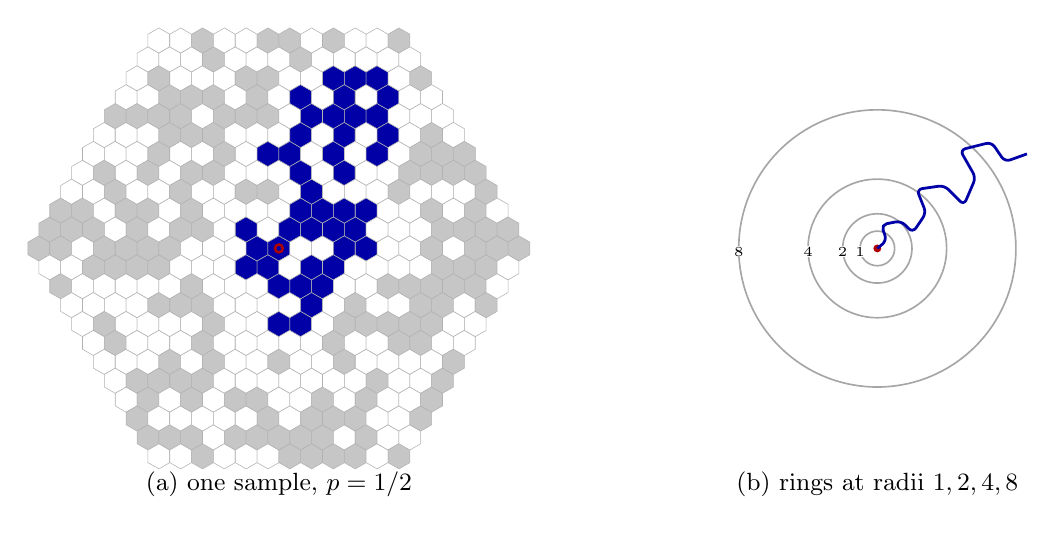
\begin{tikzpicture}
\begin{scope}
  \filldraw[fill=gray!45,draw=gray!60,line width=0.2pt] (-2.910,0.080) -- (-3.048,0.160) -- (-3.187,0.080) -- (-3.187,-0.080) -- (-3.048,-0.160) -- (-2.910,-0.080) -- cycle;
  \filldraw[fill=gray!45,draw=gray!60,line width=0.2pt] (-2.771,0.320) -- (-2.910,0.400) -- (-3.048,0.320) -- (-3.048,0.160) -- (-2.910,0.080) -- (-2.771,0.160) -- cycle;
  \filldraw[fill=gray!45,draw=gray!60,line width=0.2pt] (-2.633,0.560) -- (-2.771,0.640) -- (-2.910,0.560) -- (-2.910,0.400) -- (-2.771,0.320) -- (-2.633,0.400) -- cycle;
  \filldraw[fill=white,draw=gray!60,line width=0.2pt] (-2.494,0.800) -- (-2.633,0.880) -- (-2.771,0.800) -- (-2.771,0.640) -- (-2.633,0.560) -- (-2.494,0.640) -- cycle;
  \filldraw[fill=white,draw=gray!60,line width=0.2pt] (-2.356,1.040) -- (-2.494,1.120) -- (-2.633,1.040) -- (-2.633,0.880) -- (-2.494,0.800) -- (-2.356,0.880) -- cycle;
  \filldraw[fill=white,draw=gray!60,line width=0.2pt] (-2.217,1.280) -- (-2.356,1.360) -- (-2.494,1.280) -- (-2.494,1.120) -- (-2.356,1.040) -- (-2.217,1.120) -- cycle;
  \filldraw[fill=white,draw=gray!60,line width=0.2pt] (-2.078,1.520) -- (-2.217,1.600) -- (-2.356,1.520) -- (-2.356,1.360) -- (-2.217,1.280) -- (-2.078,1.360) -- cycle;
  \filldraw[fill=gray!45,draw=gray!60,line width=0.2pt] (-1.940,1.760) -- (-2.078,1.840) -- (-2.217,1.760) -- (-2.217,1.600) -- (-2.078,1.520) -- (-1.940,1.600) -- cycle;
  \filldraw[fill=white,draw=gray!60,line width=0.2pt] (-1.801,2.000) -- (-1.940,2.080) -- (-2.078,2.000) -- (-2.078,1.840) -- (-1.940,1.760) -- (-1.801,1.840) -- cycle;
  \filldraw[fill=white,draw=gray!60,line width=0.2pt] (-1.663,2.240) -- (-1.801,2.320) -- (-1.940,2.240) -- (-1.940,2.080) -- (-1.801,2.000) -- (-1.663,2.080) -- cycle;
  \filldraw[fill=white,draw=gray!60,line width=0.2pt] (-1.524,2.480) -- (-1.663,2.560) -- (-1.801,2.480) -- (-1.801,2.320) -- (-1.663,2.240) -- (-1.524,2.320) -- cycle;
  \filldraw[fill=white,draw=gray!60,line width=0.2pt] (-1.386,2.720) -- (-1.524,2.800) -- (-1.663,2.720) -- (-1.663,2.560) -- (-1.524,2.480) -- (-1.386,2.560) -- cycle;
  \filldraw[fill=white,draw=gray!60,line width=0.2pt] (-2.771,-0.160) -- (-2.910,-0.080) -- (-3.048,-0.160) -- (-3.048,-0.320) -- (-2.910,-0.400) -- (-2.771,-0.320) -- cycle;
  \filldraw[fill=gray!45,draw=gray!60,line width=0.2pt] (-2.633,0.080) -- (-2.771,0.160) -- (-2.910,0.080) -- (-2.910,-0.080) -- (-2.771,-0.160) -- (-2.633,-0.080) -- cycle;
  \filldraw[fill=gray!45,draw=gray!60,line width=0.2pt] (-2.494,0.320) -- (-2.633,0.400) -- (-2.771,0.320) -- (-2.771,0.160) -- (-2.633,0.080) -- (-2.494,0.160) -- cycle;
  \filldraw[fill=gray!45,draw=gray!60,line width=0.2pt] (-2.356,0.560) -- (-2.494,0.640) -- (-2.633,0.560) -- (-2.633,0.400) -- (-2.494,0.320) -- (-2.356,0.400) -- cycle;
  \filldraw[fill=white,draw=gray!60,line width=0.2pt] (-2.217,0.800) -- (-2.356,0.880) -- (-2.494,0.800) -- (-2.494,0.640) -- (-2.356,0.560) -- (-2.217,0.640) -- cycle;
  \filldraw[fill=gray!45,draw=gray!60,line width=0.2pt] (-2.078,1.040) -- (-2.217,1.120) -- (-2.356,1.040) -- (-2.356,0.880) -- (-2.217,0.800) -- (-2.078,0.880) -- cycle;
  \filldraw[fill=white,draw=gray!60,line width=0.2pt] (-1.940,1.280) -- (-2.078,1.360) -- (-2.217,1.280) -- (-2.217,1.120) -- (-2.078,1.040) -- (-1.940,1.120) -- cycle;
  \filldraw[fill=white,draw=gray!60,line width=0.2pt] (-1.801,1.520) -- (-1.940,1.600) -- (-2.078,1.520) -- (-2.078,1.360) -- (-1.940,1.280) -- (-1.801,1.360) -- cycle;
  \filldraw[fill=gray!45,draw=gray!60,line width=0.2pt] (-1.663,1.760) -- (-1.801,1.840) -- (-1.940,1.760) -- (-1.940,1.600) -- (-1.801,1.520) -- (-1.663,1.600) -- cycle;
  \filldraw[fill=white,draw=gray!60,line width=0.2pt] (-1.524,2.000) -- (-1.663,2.080) -- (-1.801,2.000) -- (-1.801,1.840) -- (-1.663,1.760) -- (-1.524,1.840) -- cycle;
  \filldraw[fill=gray!45,draw=gray!60,line width=0.2pt] (-1.386,2.240) -- (-1.524,2.320) -- (-1.663,2.240) -- (-1.663,2.080) -- (-1.524,2.000) -- (-1.386,2.080) -- cycle;
  \filldraw[fill=white,draw=gray!60,line width=0.2pt] (-1.247,2.480) -- (-1.386,2.560) -- (-1.524,2.480) -- (-1.524,2.320) -- (-1.386,2.240) -- (-1.247,2.320) -- cycle;
  \filldraw[fill=white,draw=gray!60,line width=0.2pt] (-1.109,2.720) -- (-1.247,2.800) -- (-1.386,2.720) -- (-1.386,2.560) -- (-1.247,2.480) -- (-1.109,2.560) -- cycle;
  \filldraw[fill=gray!45,draw=gray!60,line width=0.2pt] (-2.633,-0.400) -- (-2.771,-0.320) -- (-2.910,-0.400) -- (-2.910,-0.560) -- (-2.771,-0.640) -- (-2.633,-0.560) -- cycle;
  \filldraw[fill=white,draw=gray!60,line width=0.2pt] (-2.494,-0.160) -- (-2.633,-0.080) -- (-2.771,-0.160) -- (-2.771,-0.320) -- (-2.633,-0.400) -- (-2.494,-0.320) -- cycle;
  \filldraw[fill=white,draw=gray!60,line width=0.2pt] (-2.356,0.080) -- (-2.494,0.160) -- (-2.633,0.080) -- (-2.633,-0.080) -- (-2.494,-0.160) -- (-2.356,-0.080) -- cycle;
  \filldraw[fill=gray!45,draw=gray!60,line width=0.2pt] (-2.217,0.320) -- (-2.356,0.400) -- (-2.494,0.320) -- (-2.494,0.160) -- (-2.356,0.080) -- (-2.217,0.160) -- cycle;
  \filldraw[fill=white,draw=gray!60,line width=0.2pt] (-2.078,0.560) -- (-2.217,0.640) -- (-2.356,0.560) -- (-2.356,0.400) -- (-2.217,0.320) -- (-2.078,0.400) -- cycle;
  \filldraw[fill=gray!45,draw=gray!60,line width=0.2pt] (-1.940,0.800) -- (-2.078,0.880) -- (-2.217,0.800) -- (-2.217,0.640) -- (-2.078,0.560) -- (-1.940,0.640) -- cycle;
  \filldraw[fill=white,draw=gray!60,line width=0.2pt] (-1.801,1.040) -- (-1.940,1.120) -- (-2.078,1.040) -- (-2.078,0.880) -- (-1.940,0.800) -- (-1.801,0.880) -- cycle;
  \filldraw[fill=white,draw=gray!60,line width=0.2pt] (-1.663,1.280) -- (-1.801,1.360) -- (-1.940,1.280) -- (-1.940,1.120) -- (-1.801,1.040) -- (-1.663,1.120) -- cycle;
  \filldraw[fill=white,draw=gray!60,line width=0.2pt] (-1.524,1.520) -- (-1.663,1.600) -- (-1.801,1.520) -- (-1.801,1.360) -- (-1.663,1.280) -- (-1.524,1.360) -- cycle;
  \filldraw[fill=gray!45,draw=gray!60,line width=0.2pt] (-1.386,1.760) -- (-1.524,1.840) -- (-1.663,1.760) -- (-1.663,1.600) -- (-1.524,1.520) -- (-1.386,1.600) -- cycle;
  \filldraw[fill=gray!45,draw=gray!60,line width=0.2pt] (-1.247,2.000) -- (-1.386,2.080) -- (-1.524,2.000) -- (-1.524,1.840) -- (-1.386,1.760) -- (-1.247,1.840) -- cycle;
  \filldraw[fill=white,draw=gray!60,line width=0.2pt] (-1.109,2.240) -- (-1.247,2.320) -- (-1.386,2.240) -- (-1.386,2.080) -- (-1.247,2.000) -- (-1.109,2.080) -- cycle;
  \filldraw[fill=white,draw=gray!60,line width=0.2pt] (-0.970,2.480) -- (-1.109,2.560) -- (-1.247,2.480) -- (-1.247,2.320) -- (-1.109,2.240) -- (-0.970,2.320) -- cycle;
  \filldraw[fill=gray!45,draw=gray!60,line width=0.2pt] (-0.831,2.720) -- (-0.970,2.800) -- (-1.109,2.720) -- (-1.109,2.560) -- (-0.970,2.480) -- (-0.831,2.560) -- cycle;
  \filldraw[fill=white,draw=gray!60,line width=0.2pt] (-2.494,-0.640) -- (-2.633,-0.560) -- (-2.771,-0.640) -- (-2.771,-0.800) -- (-2.633,-0.880) -- (-2.494,-0.800) -- cycle;
  \filldraw[fill=white,draw=gray!60,line width=0.2pt] (-2.356,-0.400) -- (-2.494,-0.320) -- (-2.633,-0.400) -- (-2.633,-0.560) -- (-2.494,-0.640) -- (-2.356,-0.560) -- cycle;
  \filldraw[fill=gray!45,draw=gray!60,line width=0.2pt] (-2.217,-0.160) -- (-2.356,-0.080) -- (-2.494,-0.160) -- (-2.494,-0.320) -- (-2.356,-0.400) -- (-2.217,-0.320) -- cycle;
  \filldraw[fill=gray!45,draw=gray!60,line width=0.2pt] (-2.078,0.080) -- (-2.217,0.160) -- (-2.356,0.080) -- (-2.356,-0.080) -- (-2.217,-0.160) -- (-2.078,-0.080) -- cycle;
  \filldraw[fill=white,draw=gray!60,line width=0.2pt] (-1.940,0.320) -- (-2.078,0.400) -- (-2.217,0.320) -- (-2.217,0.160) -- (-2.078,0.080) -- (-1.940,0.160) -- cycle;
  \filldraw[fill=gray!45,draw=gray!60,line width=0.2pt] (-1.801,0.560) -- (-1.940,0.640) -- (-2.078,0.560) -- (-2.078,0.400) -- (-1.940,0.320) -- (-1.801,0.400) -- cycle;
  \filldraw[fill=white,draw=gray!60,line width=0.2pt] (-1.663,0.800) -- (-1.801,0.880) -- (-1.940,0.800) -- (-1.940,0.640) -- (-1.801,0.560) -- (-1.663,0.640) -- cycle;
  \filldraw[fill=gray!45,draw=gray!60,line width=0.2pt] (-1.524,1.040) -- (-1.663,1.120) -- (-1.801,1.040) -- (-1.801,0.880) -- (-1.663,0.800) -- (-1.524,0.880) -- cycle;
  \filldraw[fill=gray!45,draw=gray!60,line width=0.2pt] (-1.386,1.280) -- (-1.524,1.360) -- (-1.663,1.280) -- (-1.663,1.120) -- (-1.524,1.040) -- (-1.386,1.120) -- cycle;
  \filldraw[fill=gray!45,draw=gray!60,line width=0.2pt] (-1.247,1.520) -- (-1.386,1.600) -- (-1.524,1.520) -- (-1.524,1.360) -- (-1.386,1.280) -- (-1.247,1.360) -- cycle;
  \filldraw[fill=gray!45,draw=gray!60,line width=0.2pt] (-1.109,1.760) -- (-1.247,1.840) -- (-1.386,1.760) -- (-1.386,1.600) -- (-1.247,1.520) -- (-1.109,1.600) -- cycle;
  \filldraw[fill=gray!45,draw=gray!60,line width=0.2pt] (-0.970,2.000) -- (-1.109,2.080) -- (-1.247,2.000) -- (-1.247,1.840) -- (-1.109,1.760) -- (-0.970,1.840) -- cycle;
  \filldraw[fill=white,draw=gray!60,line width=0.2pt] (-0.831,2.240) -- (-0.970,2.320) -- (-1.109,2.240) -- (-1.109,2.080) -- (-0.970,2.000) -- (-0.831,2.080) -- cycle;
  \filldraw[fill=gray!45,draw=gray!60,line width=0.2pt] (-0.693,2.480) -- (-0.831,2.560) -- (-0.970,2.480) -- (-0.970,2.320) -- (-0.831,2.240) -- (-0.693,2.320) -- cycle;
  \filldraw[fill=white,draw=gray!60,line width=0.2pt] (-0.554,2.720) -- (-0.693,2.800) -- (-0.831,2.720) -- (-0.831,2.560) -- (-0.693,2.480) -- (-0.554,2.560) -- cycle;
  \filldraw[fill=white,draw=gray!60,line width=0.2pt] (-2.356,-0.880) -- (-2.494,-0.800) -- (-2.633,-0.880) -- (-2.633,-1.040) -- (-2.494,-1.120) -- (-2.356,-1.040) -- cycle;
  \filldraw[fill=white,draw=gray!60,line width=0.2pt] (-2.217,-0.640) -- (-2.356,-0.560) -- (-2.494,-0.640) -- (-2.494,-0.800) -- (-2.356,-0.880) -- (-2.217,-0.800) -- cycle;
  \filldraw[fill=white,draw=gray!60,line width=0.2pt] (-2.078,-0.400) -- (-2.217,-0.320) -- (-2.356,-0.400) -- (-2.356,-0.560) -- (-2.217,-0.640) -- (-2.078,-0.560) -- cycle;
  \filldraw[fill=gray!45,draw=gray!60,line width=0.2pt] (-1.940,-0.160) -- (-2.078,-0.080) -- (-2.217,-0.160) -- (-2.217,-0.320) -- (-2.078,-0.400) -- (-1.940,-0.320) -- cycle;
  \filldraw[fill=gray!45,draw=gray!60,line width=0.2pt] (-1.801,0.080) -- (-1.940,0.160) -- (-2.078,0.080) -- (-2.078,-0.080) -- (-1.940,-0.160) -- (-1.801,-0.080) -- cycle;
  \filldraw[fill=gray!45,draw=gray!60,line width=0.2pt] (-1.663,0.320) -- (-1.801,0.400) -- (-1.940,0.320) -- (-1.940,0.160) -- (-1.801,0.080) -- (-1.663,0.160) -- cycle;
  \filldraw[fill=gray!45,draw=gray!60,line width=0.2pt] (-1.524,0.560) -- (-1.663,0.640) -- (-1.801,0.560) -- (-1.801,0.400) -- (-1.663,0.320) -- (-1.524,0.400) -- cycle;
  \filldraw[fill=white,draw=gray!60,line width=0.2pt] (-1.386,0.800) -- (-1.524,0.880) -- (-1.663,0.800) -- (-1.663,0.640) -- (-1.524,0.560) -- (-1.386,0.640) -- cycle;
  \filldraw[fill=white,draw=gray!60,line width=0.2pt] (-1.247,1.040) -- (-1.386,1.120) -- (-1.524,1.040) -- (-1.524,0.880) -- (-1.386,0.800) -- (-1.247,0.880) -- cycle;
  \filldraw[fill=white,draw=gray!60,line width=0.2pt] (-1.109,1.280) -- (-1.247,1.360) -- (-1.386,1.280) -- (-1.386,1.120) -- (-1.247,1.040) -- (-1.109,1.120) -- cycle;
  \filldraw[fill=gray!45,draw=gray!60,line width=0.2pt] (-0.970,1.520) -- (-1.109,1.600) -- (-1.247,1.520) -- (-1.247,1.360) -- (-1.109,1.280) -- (-0.970,1.360) -- cycle;
  \filldraw[fill=white,draw=gray!60,line width=0.2pt] (-0.831,1.760) -- (-0.970,1.840) -- (-1.109,1.760) -- (-1.109,1.600) -- (-0.970,1.520) -- (-0.831,1.600) -- cycle;
  \filldraw[fill=gray!45,draw=gray!60,line width=0.2pt] (-0.693,2.000) -- (-0.831,2.080) -- (-0.970,2.000) -- (-0.970,1.840) -- (-0.831,1.760) -- (-0.693,1.840) -- cycle;
  \filldraw[fill=white,draw=gray!60,line width=0.2pt] (-0.554,2.240) -- (-0.693,2.320) -- (-0.831,2.240) -- (-0.831,2.080) -- (-0.693,2.000) -- (-0.554,2.080) -- cycle;
  \filldraw[fill=white,draw=gray!60,line width=0.2pt] (-0.416,2.480) -- (-0.554,2.560) -- (-0.693,2.480) -- (-0.693,2.320) -- (-0.554,2.240) -- (-0.416,2.320) -- cycle;
  \filldraw[fill=white,draw=gray!60,line width=0.2pt] (-0.277,2.720) -- (-0.416,2.800) -- (-0.554,2.720) -- (-0.554,2.560) -- (-0.416,2.480) -- (-0.277,2.560) -- cycle;
  \filldraw[fill=white,draw=gray!60,line width=0.2pt] (-2.217,-1.120) -- (-2.356,-1.040) -- (-2.494,-1.120) -- (-2.494,-1.280) -- (-2.356,-1.360) -- (-2.217,-1.280) -- cycle;
  \filldraw[fill=gray!45,draw=gray!60,line width=0.2pt] (-2.078,-0.880) -- (-2.217,-0.800) -- (-2.356,-0.880) -- (-2.356,-1.040) -- (-2.217,-1.120) -- (-2.078,-1.040) -- cycle;
  \filldraw[fill=white,draw=gray!60,line width=0.2pt] (-1.940,-0.640) -- (-2.078,-0.560) -- (-2.217,-0.640) -- (-2.217,-0.800) -- (-2.078,-0.880) -- (-1.940,-0.800) -- cycle;
  \filldraw[fill=white,draw=gray!60,line width=0.2pt] (-1.801,-0.400) -- (-1.940,-0.320) -- (-2.078,-0.400) -- (-2.078,-0.560) -- (-1.940,-0.640) -- (-1.801,-0.560) -- cycle;
  \filldraw[fill=gray!45,draw=gray!60,line width=0.2pt] (-1.663,-0.160) -- (-1.801,-0.080) -- (-1.940,-0.160) -- (-1.940,-0.320) -- (-1.801,-0.400) -- (-1.663,-0.320) -- cycle;
  \filldraw[fill=gray!45,draw=gray!60,line width=0.2pt] (-1.524,0.080) -- (-1.663,0.160) -- (-1.801,0.080) -- (-1.801,-0.080) -- (-1.663,-0.160) -- (-1.524,-0.080) -- cycle;
  \filldraw[fill=white,draw=gray!60,line width=0.2pt] (-1.386,0.320) -- (-1.524,0.400) -- (-1.663,0.320) -- (-1.663,0.160) -- (-1.524,0.080) -- (-1.386,0.160) -- cycle;
  \filldraw[fill=white,draw=gray!60,line width=0.2pt] (-1.247,0.560) -- (-1.386,0.640) -- (-1.524,0.560) -- (-1.524,0.400) -- (-1.386,0.320) -- (-1.247,0.400) -- cycle;
  \filldraw[fill=gray!45,draw=gray!60,line width=0.2pt] (-1.109,0.800) -- (-1.247,0.880) -- (-1.386,0.800) -- (-1.386,0.640) -- (-1.247,0.560) -- (-1.109,0.640) -- cycle;
  \filldraw[fill=gray!45,draw=gray!60,line width=0.2pt] (-0.970,1.040) -- (-1.109,1.120) -- (-1.247,1.040) -- (-1.247,0.880) -- (-1.109,0.800) -- (-0.970,0.880) -- cycle;
  \filldraw[fill=white,draw=gray!60,line width=0.2pt] (-0.831,1.280) -- (-0.970,1.360) -- (-1.109,1.280) -- (-1.109,1.120) -- (-0.970,1.040) -- (-0.831,1.120) -- cycle;
  \filldraw[fill=gray!45,draw=gray!60,line width=0.2pt] (-0.693,1.520) -- (-0.831,1.600) -- (-0.970,1.520) -- (-0.970,1.360) -- (-0.831,1.280) -- (-0.693,1.360) -- cycle;
  \filldraw[fill=gray!45,draw=gray!60,line width=0.2pt] (-0.554,1.760) -- (-0.693,1.840) -- (-0.831,1.760) -- (-0.831,1.600) -- (-0.693,1.520) -- (-0.554,1.600) -- cycle;
  \filldraw[fill=white,draw=gray!60,line width=0.2pt] (-0.416,2.000) -- (-0.554,2.080) -- (-0.693,2.000) -- (-0.693,1.840) -- (-0.554,1.760) -- (-0.416,1.840) -- cycle;
  \filldraw[fill=gray!45,draw=gray!60,line width=0.2pt] (-0.277,2.240) -- (-0.416,2.320) -- (-0.554,2.240) -- (-0.554,2.080) -- (-0.416,2.000) -- (-0.277,2.080) -- cycle;
  \filldraw[fill=white,draw=gray!60,line width=0.2pt] (-0.139,2.480) -- (-0.277,2.560) -- (-0.416,2.480) -- (-0.416,2.320) -- (-0.277,2.240) -- (-0.139,2.320) -- cycle;
  \filldraw[fill=gray!45,draw=gray!60,line width=0.2pt] (0.000,2.720) -- (-0.139,2.800) -- (-0.277,2.720) -- (-0.277,2.560) -- (-0.139,2.480) -- (-0.000,2.560) -- cycle;
  \filldraw[fill=white,draw=gray!60,line width=0.2pt] (-2.078,-1.360) -- (-2.217,-1.280) -- (-2.356,-1.360) -- (-2.356,-1.520) -- (-2.217,-1.600) -- (-2.078,-1.520) -- cycle;
  \filldraw[fill=gray!45,draw=gray!60,line width=0.2pt] (-1.940,-1.120) -- (-2.078,-1.040) -- (-2.217,-1.120) -- (-2.217,-1.280) -- (-2.078,-1.360) -- (-1.940,-1.280) -- cycle;
  \filldraw[fill=white,draw=gray!60,line width=0.2pt] (-1.801,-0.880) -- (-1.940,-0.800) -- (-2.078,-0.880) -- (-2.078,-1.040) -- (-1.940,-1.120) -- (-1.801,-1.040) -- cycle;
  \filldraw[fill=white,draw=gray!60,line width=0.2pt] (-1.663,-0.640) -- (-1.801,-0.560) -- (-1.940,-0.640) -- (-1.940,-0.800) -- (-1.801,-0.880) -- (-1.663,-0.800) -- cycle;
  \filldraw[fill=white,draw=gray!60,line width=0.2pt] (-1.524,-0.400) -- (-1.663,-0.320) -- (-1.801,-0.400) -- (-1.801,-0.560) -- (-1.663,-0.640) -- (-1.524,-0.560) -- cycle;
  \filldraw[fill=gray!45,draw=gray!60,line width=0.2pt] (-1.386,-0.160) -- (-1.524,-0.080) -- (-1.663,-0.160) -- (-1.663,-0.320) -- (-1.524,-0.400) -- (-1.386,-0.320) -- cycle;
  \filldraw[fill=gray!45,draw=gray!60,line width=0.2pt] (-1.247,0.080) -- (-1.386,0.160) -- (-1.524,0.080) -- (-1.524,-0.080) -- (-1.386,-0.160) -- (-1.247,-0.080) -- cycle;
  \filldraw[fill=gray!45,draw=gray!60,line width=0.2pt] (-1.109,0.320) -- (-1.247,0.400) -- (-1.386,0.320) -- (-1.386,0.160) -- (-1.247,0.080) -- (-1.109,0.160) -- cycle;
  \filldraw[fill=gray!45,draw=gray!60,line width=0.2pt] (-0.970,0.560) -- (-1.109,0.640) -- (-1.247,0.560) -- (-1.247,0.400) -- (-1.109,0.320) -- (-0.970,0.400) -- cycle;
  \filldraw[fill=white,draw=gray!60,line width=0.2pt] (-0.831,0.800) -- (-0.970,0.880) -- (-1.109,0.800) -- (-1.109,0.640) -- (-0.970,0.560) -- (-0.831,0.640) -- cycle;
  \filldraw[fill=gray!45,draw=gray!60,line width=0.2pt] (-0.693,1.040) -- (-0.831,1.120) -- (-0.970,1.040) -- (-0.970,0.880) -- (-0.831,0.800) -- (-0.693,0.880) -- cycle;
  \filldraw[fill=gray!45,draw=gray!60,line width=0.2pt] (-0.554,1.280) -- (-0.693,1.360) -- (-0.831,1.280) -- (-0.831,1.120) -- (-0.693,1.040) -- (-0.554,1.120) -- cycle;
  \filldraw[fill=white,draw=gray!60,line width=0.2pt] (-0.416,1.520) -- (-0.554,1.600) -- (-0.693,1.520) -- (-0.693,1.360) -- (-0.554,1.280) -- (-0.416,1.360) -- cycle;
  \filldraw[fill=gray!45,draw=gray!60,line width=0.2pt] (-0.277,1.760) -- (-0.416,1.840) -- (-0.554,1.760) -- (-0.554,1.600) -- (-0.416,1.520) -- (-0.277,1.600) -- cycle;
  \filldraw[fill=gray!45,draw=gray!60,line width=0.2pt] (-0.139,2.000) -- (-0.277,2.080) -- (-0.416,2.000) -- (-0.416,1.840) -- (-0.277,1.760) -- (-0.139,1.840) -- cycle;
  \filldraw[fill=gray!45,draw=gray!60,line width=0.2pt] (0.000,2.240) -- (-0.139,2.320) -- (-0.277,2.240) -- (-0.277,2.080) -- (-0.139,2.000) -- (-0.000,2.080) -- cycle;
  \filldraw[fill=white,draw=gray!60,line width=0.2pt] (0.139,2.480) -- (0.000,2.560) -- (-0.139,2.480) -- (-0.139,2.320) -- (-0.000,2.240) -- (0.139,2.320) -- cycle;
  \filldraw[fill=gray!45,draw=gray!60,line width=0.2pt] (0.277,2.720) -- (0.139,2.800) -- (0.000,2.720) -- (0.000,2.560) -- (0.139,2.480) -- (0.277,2.560) -- cycle;
  \filldraw[fill=white,draw=gray!60,line width=0.2pt] (-1.940,-1.600) -- (-2.078,-1.520) -- (-2.217,-1.600) -- (-2.217,-1.760) -- (-2.078,-1.840) -- (-1.940,-1.760) -- cycle;
  \filldraw[fill=white,draw=gray!60,line width=0.2pt] (-1.801,-1.360) -- (-1.940,-1.280) -- (-2.078,-1.360) -- (-2.078,-1.520) -- (-1.940,-1.600) -- (-1.801,-1.520) -- cycle;
  \filldraw[fill=white,draw=gray!60,line width=0.2pt] (-1.663,-1.120) -- (-1.801,-1.040) -- (-1.940,-1.120) -- (-1.940,-1.280) -- (-1.801,-1.360) -- (-1.663,-1.280) -- cycle;
  \filldraw[fill=white,draw=gray!60,line width=0.2pt] (-1.524,-0.880) -- (-1.663,-0.800) -- (-1.801,-0.880) -- (-1.801,-1.040) -- (-1.663,-1.120) -- (-1.524,-1.040) -- cycle;
  \filldraw[fill=gray!45,draw=gray!60,line width=0.2pt] (-1.386,-0.640) -- (-1.524,-0.560) -- (-1.663,-0.640) -- (-1.663,-0.800) -- (-1.524,-0.880) -- (-1.386,-0.800) -- cycle;
  \filldraw[fill=white,draw=gray!60,line width=0.2pt] (-1.247,-0.400) -- (-1.386,-0.320) -- (-1.524,-0.400) -- (-1.524,-0.560) -- (-1.386,-0.640) -- (-1.247,-0.560) -- cycle;
  \filldraw[fill=white,draw=gray!60,line width=0.2pt] (-1.109,-0.160) -- (-1.247,-0.080) -- (-1.386,-0.160) -- (-1.386,-0.320) -- (-1.247,-0.400) -- (-1.109,-0.320) -- cycle;
  \filldraw[fill=white,draw=gray!60,line width=0.2pt] (-0.970,0.080) -- (-1.109,0.160) -- (-1.247,0.080) -- (-1.247,-0.080) -- (-1.109,-0.160) -- (-0.970,-0.080) -- cycle;
  \filldraw[fill=gray!45,draw=gray!60,line width=0.2pt] (-0.831,0.320) -- (-0.970,0.400) -- (-1.109,0.320) -- (-1.109,0.160) -- (-0.970,0.080) -- (-0.831,0.160) -- cycle;
  \filldraw[fill=white,draw=gray!60,line width=0.2pt] (-0.693,0.560) -- (-0.831,0.640) -- (-0.970,0.560) -- (-0.970,0.400) -- (-0.831,0.320) -- (-0.693,0.400) -- cycle;
  \filldraw[fill=white,draw=gray!60,line width=0.2pt] (-0.554,0.800) -- (-0.693,0.880) -- (-0.831,0.800) -- (-0.831,0.640) -- (-0.693,0.560) -- (-0.554,0.640) -- cycle;
  \filldraw[fill=white,draw=gray!60,line width=0.2pt] (-0.416,1.040) -- (-0.554,1.120) -- (-0.693,1.040) -- (-0.693,0.880) -- (-0.554,0.800) -- (-0.416,0.880) -- cycle;
  \filldraw[fill=white,draw=gray!60,line width=0.2pt] (-0.277,1.280) -- (-0.416,1.360) -- (-0.554,1.280) -- (-0.554,1.120) -- (-0.416,1.040) -- (-0.277,1.120) -- cycle;
  \filldraw[fill=white,draw=gray!60,line width=0.2pt] (-0.139,1.520) -- (-0.277,1.600) -- (-0.416,1.520) -- (-0.416,1.360) -- (-0.277,1.280) -- (-0.139,1.360) -- cycle;
  \filldraw[fill=gray!45,draw=gray!60,line width=0.2pt] (0.000,1.760) -- (-0.139,1.840) -- (-0.277,1.760) -- (-0.277,1.600) -- (-0.139,1.520) -- (-0.000,1.600) -- cycle;
  \filldraw[fill=white,draw=gray!60,line width=0.2pt] (0.139,2.000) -- (0.000,2.080) -- (-0.139,2.000) -- (-0.139,1.840) -- (-0.000,1.760) -- (0.139,1.840) -- cycle;
  \filldraw[fill=white,draw=gray!60,line width=0.2pt] (0.277,2.240) -- (0.139,2.320) -- (0.000,2.240) -- (0.000,2.080) -- (0.139,2.000) -- (0.277,2.080) -- cycle;
  \filldraw[fill=gray!45,draw=gray!60,line width=0.2pt] (0.416,2.480) -- (0.277,2.560) -- (0.139,2.480) -- (0.139,2.320) -- (0.277,2.240) -- (0.416,2.320) -- cycle;
  \filldraw[fill=white,draw=gray!60,line width=0.2pt] (0.554,2.720) -- (0.416,2.800) -- (0.277,2.720) -- (0.277,2.560) -- (0.416,2.480) -- (0.554,2.560) -- cycle;
  \filldraw[fill=white,draw=gray!60,line width=0.2pt] (-1.801,-1.840) -- (-1.940,-1.760) -- (-2.078,-1.840) -- (-2.078,-2.000) -- (-1.940,-2.080) -- (-1.801,-2.000) -- cycle;
  \filldraw[fill=gray!45,draw=gray!60,line width=0.2pt] (-1.663,-1.600) -- (-1.801,-1.520) -- (-1.940,-1.600) -- (-1.940,-1.760) -- (-1.801,-1.840) -- (-1.663,-1.760) -- cycle;
  \filldraw[fill=white,draw=gray!60,line width=0.2pt] (-1.524,-1.360) -- (-1.663,-1.280) -- (-1.801,-1.360) -- (-1.801,-1.520) -- (-1.663,-1.600) -- (-1.524,-1.520) -- cycle;
  \filldraw[fill=white,draw=gray!60,line width=0.2pt] (-1.386,-1.120) -- (-1.524,-1.040) -- (-1.663,-1.120) -- (-1.663,-1.280) -- (-1.524,-1.360) -- (-1.386,-1.280) -- cycle;
  \filldraw[fill=white,draw=gray!60,line width=0.2pt] (-1.247,-0.880) -- (-1.386,-0.800) -- (-1.524,-0.880) -- (-1.524,-1.040) -- (-1.386,-1.120) -- (-1.247,-1.040) -- cycle;
  \filldraw[fill=gray!45,draw=gray!60,line width=0.2pt] (-1.109,-0.640) -- (-1.247,-0.560) -- (-1.386,-0.640) -- (-1.386,-0.800) -- (-1.247,-0.880) -- (-1.109,-0.800) -- cycle;
  \filldraw[fill=gray!45,draw=gray!60,line width=0.2pt] (-0.970,-0.400) -- (-1.109,-0.320) -- (-1.247,-0.400) -- (-1.247,-0.560) -- (-1.109,-0.640) -- (-0.970,-0.560) -- cycle;
  \filldraw[fill=white,draw=gray!60,line width=0.2pt] (-0.831,-0.160) -- (-0.970,-0.080) -- (-1.109,-0.160) -- (-1.109,-0.320) -- (-0.970,-0.400) -- (-0.831,-0.320) -- cycle;
  \filldraw[fill=white,draw=gray!60,line width=0.2pt] (-0.693,0.080) -- (-0.831,0.160) -- (-0.970,0.080) -- (-0.970,-0.080) -- (-0.831,-0.160) -- (-0.693,-0.080) -- cycle;
  \filldraw[fill=white,draw=gray!60,line width=0.2pt] (-0.554,0.320) -- (-0.693,0.400) -- (-0.831,0.320) -- (-0.831,0.160) -- (-0.693,0.080) -- (-0.554,0.160) -- cycle;
  \filldraw[fill=white,draw=gray!60,line width=0.2pt] (-0.416,0.560) -- (-0.554,0.640) -- (-0.693,0.560) -- (-0.693,0.400) -- (-0.554,0.320) -- (-0.416,0.400) -- cycle;
  \filldraw[fill=gray!45,draw=gray!60,line width=0.2pt] (-0.277,0.800) -- (-0.416,0.880) -- (-0.554,0.800) -- (-0.554,0.640) -- (-0.416,0.560) -- (-0.277,0.640) -- cycle;
  \filldraw[fill=white,draw=gray!60,line width=0.2pt] (-0.139,1.040) -- (-0.277,1.120) -- (-0.416,1.040) -- (-0.416,0.880) -- (-0.277,0.800) -- (-0.139,0.880) -- cycle;
  \filldraw[fill=blue!65!black,draw=gray!60,line width=0.2pt] (0.000,1.280) -- (-0.139,1.360) -- (-0.277,1.280) -- (-0.277,1.120) -- (-0.139,1.040) -- (-0.000,1.120) -- cycle;
  \filldraw[fill=white,draw=gray!60,line width=0.2pt] (0.139,1.520) -- (0.000,1.600) -- (-0.139,1.520) -- (-0.139,1.360) -- (-0.000,1.280) -- (0.139,1.360) -- cycle;
  \filldraw[fill=white,draw=gray!60,line width=0.2pt] (0.277,1.760) -- (0.139,1.840) -- (0.000,1.760) -- (0.000,1.600) -- (0.139,1.520) -- (0.277,1.600) -- cycle;
  \filldraw[fill=blue!65!black,draw=gray!60,line width=0.2pt] (0.416,2.000) -- (0.277,2.080) -- (0.139,2.000) -- (0.139,1.840) -- (0.277,1.760) -- (0.416,1.840) -- cycle;
  \filldraw[fill=white,draw=gray!60,line width=0.2pt] (0.554,2.240) -- (0.416,2.320) -- (0.277,2.240) -- (0.277,2.080) -- (0.416,2.000) -- (0.554,2.080) -- cycle;
  \filldraw[fill=white,draw=gray!60,line width=0.2pt] (0.693,2.480) -- (0.554,2.560) -- (0.416,2.480) -- (0.416,2.320) -- (0.554,2.240) -- (0.693,2.320) -- cycle;
  \filldraw[fill=gray!45,draw=gray!60,line width=0.2pt] (0.831,2.720) -- (0.693,2.800) -- (0.554,2.720) -- (0.554,2.560) -- (0.693,2.480) -- (0.831,2.560) -- cycle;
  \filldraw[fill=gray!45,draw=gray!60,line width=0.2pt] (-1.663,-2.080) -- (-1.801,-2.000) -- (-1.940,-2.080) -- (-1.940,-2.240) -- (-1.801,-2.320) -- (-1.663,-2.240) -- cycle;
  \filldraw[fill=gray!45,draw=gray!60,line width=0.2pt] (-1.524,-1.840) -- (-1.663,-1.760) -- (-1.801,-1.840) -- (-1.801,-2.000) -- (-1.663,-2.080) -- (-1.524,-2.000) -- cycle;
  \filldraw[fill=gray!45,draw=gray!60,line width=0.2pt] (-1.386,-1.600) -- (-1.524,-1.520) -- (-1.663,-1.600) -- (-1.663,-1.760) -- (-1.524,-1.840) -- (-1.386,-1.760) -- cycle;
  \filldraw[fill=gray!45,draw=gray!60,line width=0.2pt] (-1.247,-1.360) -- (-1.386,-1.280) -- (-1.524,-1.360) -- (-1.524,-1.520) -- (-1.386,-1.600) -- (-1.247,-1.520) -- cycle;
  \filldraw[fill=white,draw=gray!60,line width=0.2pt] (-1.109,-1.120) -- (-1.247,-1.040) -- (-1.386,-1.120) -- (-1.386,-1.280) -- (-1.247,-1.360) -- (-1.109,-1.280) -- cycle;
  \filldraw[fill=white,draw=gray!60,line width=0.2pt] (-0.970,-0.880) -- (-1.109,-0.800) -- (-1.247,-0.880) -- (-1.247,-1.040) -- (-1.109,-1.120) -- (-0.970,-1.040) -- cycle;
  \filldraw[fill=gray!45,draw=gray!60,line width=0.2pt] (-0.831,-0.640) -- (-0.970,-0.560) -- (-1.109,-0.640) -- (-1.109,-0.800) -- (-0.970,-0.880) -- (-0.831,-0.800) -- cycle;
  \filldraw[fill=white,draw=gray!60,line width=0.2pt] (-0.693,-0.400) -- (-0.831,-0.320) -- (-0.970,-0.400) -- (-0.970,-0.560) -- (-0.831,-0.640) -- (-0.693,-0.560) -- cycle;
  \filldraw[fill=white,draw=gray!60,line width=0.2pt] (-0.554,-0.160) -- (-0.693,-0.080) -- (-0.831,-0.160) -- (-0.831,-0.320) -- (-0.693,-0.400) -- (-0.554,-0.320) -- cycle;
  \filldraw[fill=white,draw=gray!60,line width=0.2pt] (-0.416,0.080) -- (-0.554,0.160) -- (-0.693,0.080) -- (-0.693,-0.080) -- (-0.554,-0.160) -- (-0.416,-0.080) -- cycle;
  \filldraw[fill=blue!65!black,draw=gray!60,line width=0.2pt] (-0.277,0.320) -- (-0.416,0.400) -- (-0.554,0.320) -- (-0.554,0.160) -- (-0.416,0.080) -- (-0.277,0.160) -- cycle;
  \filldraw[fill=white,draw=gray!60,line width=0.2pt] (-0.139,0.560) -- (-0.277,0.640) -- (-0.416,0.560) -- (-0.416,0.400) -- (-0.277,0.320) -- (-0.139,0.400) -- cycle;
  \filldraw[fill=gray!45,draw=gray!60,line width=0.2pt] (0.000,0.800) -- (-0.139,0.880) -- (-0.277,0.800) -- (-0.277,0.640) -- (-0.139,0.560) -- (-0.000,0.640) -- cycle;
  \filldraw[fill=white,draw=gray!60,line width=0.2pt] (0.139,1.040) -- (0.000,1.120) -- (-0.139,1.040) -- (-0.139,0.880) -- (-0.000,0.800) -- (0.139,0.880) -- cycle;
  \filldraw[fill=blue!65!black,draw=gray!60,line width=0.2pt] (0.277,1.280) -- (0.139,1.360) -- (0.000,1.280) -- (0.000,1.120) -- (0.139,1.040) -- (0.277,1.120) -- cycle;
  \filldraw[fill=blue!65!black,draw=gray!60,line width=0.2pt] (0.416,1.520) -- (0.277,1.600) -- (0.139,1.520) -- (0.139,1.360) -- (0.277,1.280) -- (0.416,1.360) -- cycle;
  \filldraw[fill=blue!65!black,draw=gray!60,line width=0.2pt] (0.554,1.760) -- (0.416,1.840) -- (0.277,1.760) -- (0.277,1.600) -- (0.416,1.520) -- (0.554,1.600) -- cycle;
  \filldraw[fill=white,draw=gray!60,line width=0.2pt] (0.693,2.000) -- (0.554,2.080) -- (0.416,2.000) -- (0.416,1.840) -- (0.554,1.760) -- (0.693,1.840) -- cycle;
  \filldraw[fill=blue!65!black,draw=gray!60,line width=0.2pt] (0.831,2.240) -- (0.693,2.320) -- (0.554,2.240) -- (0.554,2.080) -- (0.693,2.000) -- (0.831,2.080) -- cycle;
  \filldraw[fill=white,draw=gray!60,line width=0.2pt] (0.970,2.480) -- (0.831,2.560) -- (0.693,2.480) -- (0.693,2.320) -- (0.831,2.240) -- (0.970,2.320) -- cycle;
  \filldraw[fill=white,draw=gray!60,line width=0.2pt] (1.109,2.720) -- (0.970,2.800) -- (0.831,2.720) -- (0.831,2.560) -- (0.970,2.480) -- (1.109,2.560) -- cycle;
  \filldraw[fill=gray!45,draw=gray!60,line width=0.2pt] (-1.524,-2.320) -- (-1.663,-2.240) -- (-1.801,-2.320) -- (-1.801,-2.480) -- (-1.663,-2.560) -- (-1.524,-2.480) -- cycle;
  \filldraw[fill=white,draw=gray!60,line width=0.2pt] (-1.386,-2.080) -- (-1.524,-2.000) -- (-1.663,-2.080) -- (-1.663,-2.240) -- (-1.524,-2.320) -- (-1.386,-2.240) -- cycle;
  \filldraw[fill=white,draw=gray!60,line width=0.2pt] (-1.247,-1.840) -- (-1.386,-1.760) -- (-1.524,-1.840) -- (-1.524,-2.000) -- (-1.386,-2.080) -- (-1.247,-2.000) -- cycle;
  \filldraw[fill=gray!45,draw=gray!60,line width=0.2pt] (-1.109,-1.600) -- (-1.247,-1.520) -- (-1.386,-1.600) -- (-1.386,-1.760) -- (-1.247,-1.840) -- (-1.109,-1.760) -- cycle;
  \filldraw[fill=white,draw=gray!60,line width=0.2pt] (-0.970,-1.360) -- (-1.109,-1.280) -- (-1.247,-1.360) -- (-1.247,-1.520) -- (-1.109,-1.600) -- (-0.970,-1.520) -- cycle;
  \filldraw[fill=gray!45,draw=gray!60,line width=0.2pt] (-0.831,-1.120) -- (-0.970,-1.040) -- (-1.109,-1.120) -- (-1.109,-1.280) -- (-0.970,-1.360) -- (-0.831,-1.280) -- cycle;
  \filldraw[fill=gray!45,draw=gray!60,line width=0.2pt] (-0.693,-0.880) -- (-0.831,-0.800) -- (-0.970,-0.880) -- (-0.970,-1.040) -- (-0.831,-1.120) -- (-0.693,-1.040) -- cycle;
  \filldraw[fill=white,draw=gray!60,line width=0.2pt] (-0.554,-0.640) -- (-0.693,-0.560) -- (-0.831,-0.640) -- (-0.831,-0.800) -- (-0.693,-0.880) -- (-0.554,-0.800) -- cycle;
  \filldraw[fill=white,draw=gray!60,line width=0.2pt] (-0.416,-0.400) -- (-0.554,-0.320) -- (-0.693,-0.400) -- (-0.693,-0.560) -- (-0.554,-0.640) -- (-0.416,-0.560) -- cycle;
  \filldraw[fill=blue!65!black,draw=gray!60,line width=0.2pt] (-0.277,-0.160) -- (-0.416,-0.080) -- (-0.554,-0.160) -- (-0.554,-0.320) -- (-0.416,-0.400) -- (-0.277,-0.320) -- cycle;
  \filldraw[fill=blue!65!black,draw=gray!60,line width=0.2pt] (-0.139,0.080) -- (-0.277,0.160) -- (-0.416,0.080) -- (-0.416,-0.080) -- (-0.277,-0.160) -- (-0.139,-0.080) -- cycle;
  \filldraw[fill=white,draw=gray!60,line width=0.2pt] (0.000,0.320) -- (-0.139,0.400) -- (-0.277,0.320) -- (-0.277,0.160) -- (-0.139,0.080) -- (-0.000,0.160) -- cycle;
  \filldraw[fill=white,draw=gray!60,line width=0.2pt] (0.139,0.560) -- (0.000,0.640) -- (-0.139,0.560) -- (-0.139,0.400) -- (-0.000,0.320) -- (0.139,0.400) -- cycle;
  \filldraw[fill=white,draw=gray!60,line width=0.2pt] (0.277,0.800) -- (0.139,0.880) -- (0.000,0.800) -- (0.000,0.640) -- (0.139,0.560) -- (0.277,0.640) -- cycle;
  \filldraw[fill=blue!65!black,draw=gray!60,line width=0.2pt] (0.416,1.040) -- (0.277,1.120) -- (0.139,1.040) -- (0.139,0.880) -- (0.277,0.800) -- (0.416,0.880) -- cycle;
  \filldraw[fill=white,draw=gray!60,line width=0.2pt] (0.554,1.280) -- (0.416,1.360) -- (0.277,1.280) -- (0.277,1.120) -- (0.416,1.040) -- (0.554,1.120) -- cycle;
  \filldraw[fill=white,draw=gray!60,line width=0.2pt] (0.693,1.520) -- (0.554,1.600) -- (0.416,1.520) -- (0.416,1.360) -- (0.554,1.280) -- (0.693,1.360) -- cycle;
  \filldraw[fill=blue!65!black,draw=gray!60,line width=0.2pt] (0.831,1.760) -- (0.693,1.840) -- (0.554,1.760) -- (0.554,1.600) -- (0.693,1.520) -- (0.831,1.600) -- cycle;
  \filldraw[fill=blue!65!black,draw=gray!60,line width=0.2pt] (0.970,2.000) -- (0.831,2.080) -- (0.693,2.000) -- (0.693,1.840) -- (0.831,1.760) -- (0.970,1.840) -- cycle;
  \filldraw[fill=blue!65!black,draw=gray!60,line width=0.2pt] (1.109,2.240) -- (0.970,2.320) -- (0.831,2.240) -- (0.831,2.080) -- (0.970,2.000) -- (1.109,2.080) -- cycle;
  \filldraw[fill=white,draw=gray!60,line width=0.2pt] (1.247,2.480) -- (1.109,2.560) -- (0.970,2.480) -- (0.970,2.320) -- (1.109,2.240) -- (1.247,2.320) -- cycle;
  \filldraw[fill=white,draw=gray!60,line width=0.2pt] (1.386,2.720) -- (1.247,2.800) -- (1.109,2.720) -- (1.109,2.560) -- (1.247,2.480) -- (1.386,2.560) -- cycle;
  \filldraw[fill=white,draw=gray!60,line width=0.2pt] (-1.386,-2.560) -- (-1.524,-2.480) -- (-1.663,-2.560) -- (-1.663,-2.720) -- (-1.524,-2.800) -- (-1.386,-2.720) -- cycle;
  \filldraw[fill=gray!45,draw=gray!60,line width=0.2pt] (-1.247,-2.320) -- (-1.386,-2.240) -- (-1.524,-2.320) -- (-1.524,-2.480) -- (-1.386,-2.560) -- (-1.247,-2.480) -- cycle;
  \filldraw[fill=white,draw=gray!60,line width=0.2pt] (-1.109,-2.080) -- (-1.247,-2.000) -- (-1.386,-2.080) -- (-1.386,-2.240) -- (-1.247,-2.320) -- (-1.109,-2.240) -- cycle;
  \filldraw[fill=gray!45,draw=gray!60,line width=0.2pt] (-0.970,-1.840) -- (-1.109,-1.760) -- (-1.247,-1.840) -- (-1.247,-2.000) -- (-1.109,-2.080) -- (-0.970,-2.000) -- cycle;
  \filldraw[fill=gray!45,draw=gray!60,line width=0.2pt] (-0.831,-1.600) -- (-0.970,-1.520) -- (-1.109,-1.600) -- (-1.109,-1.760) -- (-0.970,-1.840) -- (-0.831,-1.760) -- cycle;
  \filldraw[fill=gray!45,draw=gray!60,line width=0.2pt] (-0.693,-1.360) -- (-0.831,-1.280) -- (-0.970,-1.360) -- (-0.970,-1.520) -- (-0.831,-1.600) -- (-0.693,-1.520) -- cycle;
  \filldraw[fill=white,draw=gray!60,line width=0.2pt] (-0.554,-1.120) -- (-0.693,-1.040) -- (-0.831,-1.120) -- (-0.831,-1.280) -- (-0.693,-1.360) -- (-0.554,-1.280) -- cycle;
  \filldraw[fill=white,draw=gray!60,line width=0.2pt] (-0.416,-0.880) -- (-0.554,-0.800) -- (-0.693,-0.880) -- (-0.693,-1.040) -- (-0.554,-1.120) -- (-0.416,-1.040) -- cycle;
  \filldraw[fill=white,draw=gray!60,line width=0.2pt] (-0.277,-0.640) -- (-0.416,-0.560) -- (-0.554,-0.640) -- (-0.554,-0.800) -- (-0.416,-0.880) -- (-0.277,-0.800) -- cycle;
  \filldraw[fill=white,draw=gray!60,line width=0.2pt] (-0.139,-0.400) -- (-0.277,-0.320) -- (-0.416,-0.400) -- (-0.416,-0.560) -- (-0.277,-0.640) -- (-0.139,-0.560) -- cycle;
  \filldraw[fill=blue!65!black,draw=gray!60,line width=0.2pt] (0.000,-0.160) -- (-0.139,-0.080) -- (-0.277,-0.160) -- (-0.277,-0.320) -- (-0.139,-0.400) -- (-0.000,-0.320) -- cycle;
  \filldraw[fill=blue!65!black,draw=gray!60,line width=0.2pt] (0.139,0.080) -- (0.000,0.160) -- (-0.139,0.080) -- (-0.139,-0.080) -- (-0.000,-0.160) -- (0.139,-0.080) -- cycle;
  \filldraw[fill=blue!65!black,draw=gray!60,line width=0.2pt] (0.277,0.320) -- (0.139,0.400) -- (0.000,0.320) -- (0.000,0.160) -- (0.139,0.080) -- (0.277,0.160) -- cycle;
  \filldraw[fill=blue!65!black,draw=gray!60,line width=0.2pt] (0.416,0.560) -- (0.277,0.640) -- (0.139,0.560) -- (0.139,0.400) -- (0.277,0.320) -- (0.416,0.400) -- cycle;
  \filldraw[fill=blue!65!black,draw=gray!60,line width=0.2pt] (0.554,0.800) -- (0.416,0.880) -- (0.277,0.800) -- (0.277,0.640) -- (0.416,0.560) -- (0.554,0.640) -- cycle;
  \filldraw[fill=white,draw=gray!60,line width=0.2pt] (0.693,1.040) -- (0.554,1.120) -- (0.416,1.040) -- (0.416,0.880) -- (0.554,0.800) -- (0.693,0.880) -- cycle;
  \filldraw[fill=blue!65!black,draw=gray!60,line width=0.2pt] (0.831,1.280) -- (0.693,1.360) -- (0.554,1.280) -- (0.554,1.120) -- (0.693,1.040) -- (0.831,1.120) -- cycle;
  \filldraw[fill=blue!65!black,draw=gray!60,line width=0.2pt] (0.970,1.520) -- (0.831,1.600) -- (0.693,1.520) -- (0.693,1.360) -- (0.831,1.280) -- (0.970,1.360) -- cycle;
  \filldraw[fill=blue!65!black,draw=gray!60,line width=0.2pt] (1.109,1.760) -- (0.970,1.840) -- (0.831,1.760) -- (0.831,1.600) -- (0.970,1.520) -- (1.109,1.600) -- cycle;
  \filldraw[fill=white,draw=gray!60,line width=0.2pt] (1.247,2.000) -- (1.109,2.080) -- (0.970,2.000) -- (0.970,1.840) -- (1.109,1.760) -- (1.247,1.840) -- cycle;
  \filldraw[fill=blue!65!black,draw=gray!60,line width=0.2pt] (1.386,2.240) -- (1.247,2.320) -- (1.109,2.240) -- (1.109,2.080) -- (1.247,2.000) -- (1.386,2.080) -- cycle;
  \filldraw[fill=white,draw=gray!60,line width=0.2pt] (1.524,2.480) -- (1.386,2.560) -- (1.247,2.480) -- (1.247,2.320) -- (1.386,2.240) -- (1.524,2.320) -- cycle;
  \filldraw[fill=gray!45,draw=gray!60,line width=0.2pt] (1.663,2.720) -- (1.524,2.800) -- (1.386,2.720) -- (1.386,2.560) -- (1.524,2.480) -- (1.663,2.560) -- cycle;
  \filldraw[fill=white,draw=gray!60,line width=0.2pt] (-1.109,-2.560) -- (-1.247,-2.480) -- (-1.386,-2.560) -- (-1.386,-2.720) -- (-1.247,-2.800) -- (-1.109,-2.720) -- cycle;
  \filldraw[fill=gray!45,draw=gray!60,line width=0.2pt] (-0.970,-2.320) -- (-1.109,-2.240) -- (-1.247,-2.320) -- (-1.247,-2.480) -- (-1.109,-2.560) -- (-0.970,-2.480) -- cycle;
  \filldraw[fill=white,draw=gray!60,line width=0.2pt] (-0.831,-2.080) -- (-0.970,-2.000) -- (-1.109,-2.080) -- (-1.109,-2.240) -- (-0.970,-2.320) -- (-0.831,-2.240) -- cycle;
  \filldraw[fill=white,draw=gray!60,line width=0.2pt] (-0.693,-1.840) -- (-0.831,-1.760) -- (-0.970,-1.840) -- (-0.970,-2.000) -- (-0.831,-2.080) -- (-0.693,-2.000) -- cycle;
  \filldraw[fill=white,draw=gray!60,line width=0.2pt] (-0.554,-1.600) -- (-0.693,-1.520) -- (-0.831,-1.600) -- (-0.831,-1.760) -- (-0.693,-1.840) -- (-0.554,-1.760) -- cycle;
  \filldraw[fill=white,draw=gray!60,line width=0.2pt] (-0.416,-1.360) -- (-0.554,-1.280) -- (-0.693,-1.360) -- (-0.693,-1.520) -- (-0.554,-1.600) -- (-0.416,-1.520) -- cycle;
  \filldraw[fill=white,draw=gray!60,line width=0.2pt] (-0.277,-1.120) -- (-0.416,-1.040) -- (-0.554,-1.120) -- (-0.554,-1.280) -- (-0.416,-1.360) -- (-0.277,-1.280) -- cycle;
  \filldraw[fill=white,draw=gray!60,line width=0.2pt] (-0.139,-0.880) -- (-0.277,-0.800) -- (-0.416,-0.880) -- (-0.416,-1.040) -- (-0.277,-1.120) -- (-0.139,-1.040) -- cycle;
  \filldraw[fill=white,draw=gray!60,line width=0.2pt] (0.000,-0.640) -- (-0.139,-0.560) -- (-0.277,-0.640) -- (-0.277,-0.800) -- (-0.139,-0.880) -- (-0.000,-0.800) -- cycle;
  \filldraw[fill=blue!65!black,draw=gray!60,line width=0.2pt] (0.139,-0.400) -- (0.000,-0.320) -- (-0.139,-0.400) -- (-0.139,-0.560) -- (-0.000,-0.640) -- (0.139,-0.560) -- cycle;
  \filldraw[fill=white,draw=gray!60,line width=0.2pt] (0.277,-0.160) -- (0.139,-0.080) -- (0.000,-0.160) -- (0.000,-0.320) -- (0.139,-0.400) -- (0.277,-0.320) -- cycle;
  \filldraw[fill=white,draw=gray!60,line width=0.2pt] (0.416,0.080) -- (0.277,0.160) -- (0.139,0.080) -- (0.139,-0.080) -- (0.277,-0.160) -- (0.416,-0.080) -- cycle;
  \filldraw[fill=blue!65!black,draw=gray!60,line width=0.2pt] (0.554,0.320) -- (0.416,0.400) -- (0.277,0.320) -- (0.277,0.160) -- (0.416,0.080) -- (0.554,0.160) -- cycle;
  \filldraw[fill=blue!65!black,draw=gray!60,line width=0.2pt] (0.693,0.560) -- (0.554,0.640) -- (0.416,0.560) -- (0.416,0.400) -- (0.554,0.320) -- (0.693,0.400) -- cycle;
  \filldraw[fill=white,draw=gray!60,line width=0.2pt] (0.831,0.800) -- (0.693,0.880) -- (0.554,0.800) -- (0.554,0.640) -- (0.693,0.560) -- (0.831,0.640) -- cycle;
  \filldraw[fill=blue!65!black,draw=gray!60,line width=0.2pt] (0.970,1.040) -- (0.831,1.120) -- (0.693,1.040) -- (0.693,0.880) -- (0.831,0.800) -- (0.970,0.880) -- cycle;
  \filldraw[fill=white,draw=gray!60,line width=0.2pt] (1.109,1.280) -- (0.970,1.360) -- (0.831,1.280) -- (0.831,1.120) -- (0.970,1.040) -- (1.109,1.120) -- cycle;
  \filldraw[fill=white,draw=gray!60,line width=0.2pt] (1.247,1.520) -- (1.109,1.600) -- (0.970,1.520) -- (0.970,1.360) -- (1.109,1.280) -- (1.247,1.360) -- cycle;
  \filldraw[fill=blue!65!black,draw=gray!60,line width=0.2pt] (1.386,1.760) -- (1.247,1.840) -- (1.109,1.760) -- (1.109,1.600) -- (1.247,1.520) -- (1.386,1.600) -- cycle;
  \filldraw[fill=blue!65!black,draw=gray!60,line width=0.2pt] (1.524,2.000) -- (1.386,2.080) -- (1.247,2.000) -- (1.247,1.840) -- (1.386,1.760) -- (1.524,1.840) -- cycle;
  \filldraw[fill=white,draw=gray!60,line width=0.2pt] (1.663,2.240) -- (1.524,2.320) -- (1.386,2.240) -- (1.386,2.080) -- (1.524,2.000) -- (1.663,2.080) -- cycle;
  \filldraw[fill=white,draw=gray!60,line width=0.2pt] (1.801,2.480) -- (1.663,2.560) -- (1.524,2.480) -- (1.524,2.320) -- (1.663,2.240) -- (1.801,2.320) -- cycle;
  \filldraw[fill=gray!45,draw=gray!60,line width=0.2pt] (-0.831,-2.560) -- (-0.970,-2.480) -- (-1.109,-2.560) -- (-1.109,-2.720) -- (-0.970,-2.800) -- (-0.831,-2.720) -- cycle;
  \filldraw[fill=white,draw=gray!60,line width=0.2pt] (-0.693,-2.320) -- (-0.831,-2.240) -- (-0.970,-2.320) -- (-0.970,-2.480) -- (-0.831,-2.560) -- (-0.693,-2.480) -- cycle;
  \filldraw[fill=white,draw=gray!60,line width=0.2pt] (-0.554,-2.080) -- (-0.693,-2.000) -- (-0.831,-2.080) -- (-0.831,-2.240) -- (-0.693,-2.320) -- (-0.554,-2.240) -- cycle;
  \filldraw[fill=gray!45,draw=gray!60,line width=0.2pt] (-0.416,-1.840) -- (-0.554,-1.760) -- (-0.693,-1.840) -- (-0.693,-2.000) -- (-0.554,-2.080) -- (-0.416,-2.000) -- cycle;
  \filldraw[fill=white,draw=gray!60,line width=0.2pt] (-0.277,-1.600) -- (-0.416,-1.520) -- (-0.554,-1.600) -- (-0.554,-1.760) -- (-0.416,-1.840) -- (-0.277,-1.760) -- cycle;
  \filldraw[fill=white,draw=gray!60,line width=0.2pt] (-0.139,-1.360) -- (-0.277,-1.280) -- (-0.416,-1.360) -- (-0.416,-1.520) -- (-0.277,-1.600) -- (-0.139,-1.520) -- cycle;
  \filldraw[fill=white,draw=gray!60,line width=0.2pt] (0.000,-1.120) -- (-0.139,-1.040) -- (-0.277,-1.120) -- (-0.277,-1.280) -- (-0.139,-1.360) -- (-0.000,-1.280) -- cycle;
  \filldraw[fill=blue!65!black,draw=gray!60,line width=0.2pt] (0.139,-0.880) -- (0.000,-0.800) -- (-0.139,-0.880) -- (-0.139,-1.040) -- (-0.000,-1.120) -- (0.139,-1.040) -- cycle;
  \filldraw[fill=white,draw=gray!60,line width=0.2pt] (0.277,-0.640) -- (0.139,-0.560) -- (0.000,-0.640) -- (0.000,-0.800) -- (0.139,-0.880) -- (0.277,-0.800) -- cycle;
  \filldraw[fill=blue!65!black,draw=gray!60,line width=0.2pt] (0.416,-0.400) -- (0.277,-0.320) -- (0.139,-0.400) -- (0.139,-0.560) -- (0.277,-0.640) -- (0.416,-0.560) -- cycle;
  \filldraw[fill=blue!65!black,draw=gray!60,line width=0.2pt] (0.554,-0.160) -- (0.416,-0.080) -- (0.277,-0.160) -- (0.277,-0.320) -- (0.416,-0.400) -- (0.554,-0.320) -- cycle;
  \filldraw[fill=white,draw=gray!60,line width=0.2pt] (0.693,0.080) -- (0.554,0.160) -- (0.416,0.080) -- (0.416,-0.080) -- (0.554,-0.160) -- (0.693,-0.080) -- cycle;
  \filldraw[fill=blue!65!black,draw=gray!60,line width=0.2pt] (0.831,0.320) -- (0.693,0.400) -- (0.554,0.320) -- (0.554,0.160) -- (0.693,0.080) -- (0.831,0.160) -- cycle;
  \filldraw[fill=blue!65!black,draw=gray!60,line width=0.2pt] (0.970,0.560) -- (0.831,0.640) -- (0.693,0.560) -- (0.693,0.400) -- (0.831,0.320) -- (0.970,0.400) -- cycle;
  \filldraw[fill=white,draw=gray!60,line width=0.2pt] (1.109,0.800) -- (0.970,0.880) -- (0.831,0.800) -- (0.831,0.640) -- (0.970,0.560) -- (1.109,0.640) -- cycle;
  \filldraw[fill=white,draw=gray!60,line width=0.2pt] (1.247,1.040) -- (1.109,1.120) -- (0.970,1.040) -- (0.970,0.880) -- (1.109,0.800) -- (1.247,0.880) -- cycle;
  \filldraw[fill=blue!65!black,draw=gray!60,line width=0.2pt] (1.386,1.280) -- (1.247,1.360) -- (1.109,1.280) -- (1.109,1.120) -- (1.247,1.040) -- (1.386,1.120) -- cycle;
  \filldraw[fill=blue!65!black,draw=gray!60,line width=0.2pt] (1.524,1.520) -- (1.386,1.600) -- (1.247,1.520) -- (1.247,1.360) -- (1.386,1.280) -- (1.524,1.360) -- cycle;
  \filldraw[fill=white,draw=gray!60,line width=0.2pt] (1.663,1.760) -- (1.524,1.840) -- (1.386,1.760) -- (1.386,1.600) -- (1.524,1.520) -- (1.663,1.600) -- cycle;
  \filldraw[fill=white,draw=gray!60,line width=0.2pt] (1.801,2.000) -- (1.663,2.080) -- (1.524,2.000) -- (1.524,1.840) -- (1.663,1.760) -- (1.801,1.840) -- cycle;
  \filldraw[fill=gray!45,draw=gray!60,line width=0.2pt] (1.940,2.240) -- (1.801,2.320) -- (1.663,2.240) -- (1.663,2.080) -- (1.801,2.000) -- (1.940,2.080) -- cycle;
  \filldraw[fill=white,draw=gray!60,line width=0.2pt] (-0.554,-2.560) -- (-0.693,-2.480) -- (-0.831,-2.560) -- (-0.831,-2.720) -- (-0.693,-2.800) -- (-0.554,-2.720) -- cycle;
  \filldraw[fill=gray!45,draw=gray!60,line width=0.2pt] (-0.416,-2.320) -- (-0.554,-2.240) -- (-0.693,-2.320) -- (-0.693,-2.480) -- (-0.554,-2.560) -- (-0.416,-2.480) -- cycle;
  \filldraw[fill=white,draw=gray!60,line width=0.2pt] (-0.277,-2.080) -- (-0.416,-2.000) -- (-0.554,-2.080) -- (-0.554,-2.240) -- (-0.416,-2.320) -- (-0.277,-2.240) -- cycle;
  \filldraw[fill=gray!45,draw=gray!60,line width=0.2pt] (-0.139,-1.840) -- (-0.277,-1.760) -- (-0.416,-1.840) -- (-0.416,-2.000) -- (-0.277,-2.080) -- (-0.139,-2.000) -- cycle;
  \filldraw[fill=white,draw=gray!60,line width=0.2pt] (0.000,-1.600) -- (-0.139,-1.520) -- (-0.277,-1.600) -- (-0.277,-1.760) -- (-0.139,-1.840) -- (-0.000,-1.760) -- cycle;
  \filldraw[fill=gray!45,draw=gray!60,line width=0.2pt] (0.139,-1.360) -- (0.000,-1.280) -- (-0.139,-1.360) -- (-0.139,-1.520) -- (-0.000,-1.600) -- (0.139,-1.520) -- cycle;
  \filldraw[fill=white,draw=gray!60,line width=0.2pt] (0.277,-1.120) -- (0.139,-1.040) -- (0.000,-1.120) -- (0.000,-1.280) -- (0.139,-1.360) -- (0.277,-1.280) -- cycle;
  \filldraw[fill=blue!65!black,draw=gray!60,line width=0.2pt] (0.416,-0.880) -- (0.277,-0.800) -- (0.139,-0.880) -- (0.139,-1.040) -- (0.277,-1.120) -- (0.416,-1.040) -- cycle;
  \filldraw[fill=blue!65!black,draw=gray!60,line width=0.2pt] (0.554,-0.640) -- (0.416,-0.560) -- (0.277,-0.640) -- (0.277,-0.800) -- (0.416,-0.880) -- (0.554,-0.800) -- cycle;
  \filldraw[fill=blue!65!black,draw=gray!60,line width=0.2pt] (0.693,-0.400) -- (0.554,-0.320) -- (0.416,-0.400) -- (0.416,-0.560) -- (0.554,-0.640) -- (0.693,-0.560) -- cycle;
  \filldraw[fill=blue!65!black,draw=gray!60,line width=0.2pt] (0.831,-0.160) -- (0.693,-0.080) -- (0.554,-0.160) -- (0.554,-0.320) -- (0.693,-0.400) -- (0.831,-0.320) -- cycle;
  \filldraw[fill=blue!65!black,draw=gray!60,line width=0.2pt] (0.970,0.080) -- (0.831,0.160) -- (0.693,0.080) -- (0.693,-0.080) -- (0.831,-0.160) -- (0.970,-0.080) -- cycle;
  \filldraw[fill=blue!65!black,draw=gray!60,line width=0.2pt] (1.109,0.320) -- (0.970,0.400) -- (0.831,0.320) -- (0.831,0.160) -- (0.970,0.080) -- (1.109,0.160) -- cycle;
  \filldraw[fill=blue!65!black,draw=gray!60,line width=0.2pt] (1.247,0.560) -- (1.109,0.640) -- (0.970,0.560) -- (0.970,0.400) -- (1.109,0.320) -- (1.247,0.400) -- cycle;
  \filldraw[fill=white,draw=gray!60,line width=0.2pt] (1.386,0.800) -- (1.247,0.880) -- (1.109,0.800) -- (1.109,0.640) -- (1.247,0.560) -- (1.386,0.640) -- cycle;
  \filldraw[fill=white,draw=gray!60,line width=0.2pt] (1.524,1.040) -- (1.386,1.120) -- (1.247,1.040) -- (1.247,0.880) -- (1.386,0.800) -- (1.524,0.880) -- cycle;
  \filldraw[fill=white,draw=gray!60,line width=0.2pt] (1.663,1.280) -- (1.524,1.360) -- (1.386,1.280) -- (1.386,1.120) -- (1.524,1.040) -- (1.663,1.120) -- cycle;
  \filldraw[fill=white,draw=gray!60,line width=0.2pt] (1.801,1.520) -- (1.663,1.600) -- (1.524,1.520) -- (1.524,1.360) -- (1.663,1.280) -- (1.801,1.360) -- cycle;
  \filldraw[fill=white,draw=gray!60,line width=0.2pt] (1.940,1.760) -- (1.801,1.840) -- (1.663,1.760) -- (1.663,1.600) -- (1.801,1.520) -- (1.940,1.600) -- cycle;
  \filldraw[fill=white,draw=gray!60,line width=0.2pt] (2.078,2.000) -- (1.940,2.080) -- (1.801,2.000) -- (1.801,1.840) -- (1.940,1.760) -- (2.078,1.840) -- cycle;
  \filldraw[fill=white,draw=gray!60,line width=0.2pt] (-0.277,-2.560) -- (-0.416,-2.480) -- (-0.554,-2.560) -- (-0.554,-2.720) -- (-0.416,-2.800) -- (-0.277,-2.720) -- cycle;
  \filldraw[fill=gray!45,draw=gray!60,line width=0.2pt] (-0.139,-2.320) -- (-0.277,-2.240) -- (-0.416,-2.320) -- (-0.416,-2.480) -- (-0.277,-2.560) -- (-0.139,-2.480) -- cycle;
  \filldraw[fill=gray!45,draw=gray!60,line width=0.2pt] (0.000,-2.080) -- (-0.139,-2.000) -- (-0.277,-2.080) -- (-0.277,-2.240) -- (-0.139,-2.320) -- (-0.000,-2.240) -- cycle;
  \filldraw[fill=white,draw=gray!60,line width=0.2pt] (0.139,-1.840) -- (0.000,-1.760) -- (-0.139,-1.840) -- (-0.139,-2.000) -- (-0.000,-2.080) -- (0.139,-2.000) -- cycle;
  \filldraw[fill=white,draw=gray!60,line width=0.2pt] (0.277,-1.600) -- (0.139,-1.520) -- (0.000,-1.600) -- (0.000,-1.760) -- (0.139,-1.840) -- (0.277,-1.760) -- cycle;
  \filldraw[fill=white,draw=gray!60,line width=0.2pt] (0.416,-1.360) -- (0.277,-1.280) -- (0.139,-1.360) -- (0.139,-1.520) -- (0.277,-1.600) -- (0.416,-1.520) -- cycle;
  \filldraw[fill=white,draw=gray!60,line width=0.2pt] (0.554,-1.120) -- (0.416,-1.040) -- (0.277,-1.120) -- (0.277,-1.280) -- (0.416,-1.360) -- (0.554,-1.280) -- cycle;
  \filldraw[fill=white,draw=gray!60,line width=0.2pt] (0.693,-0.880) -- (0.554,-0.800) -- (0.416,-0.880) -- (0.416,-1.040) -- (0.554,-1.120) -- (0.693,-1.040) -- cycle;
  \filldraw[fill=white,draw=gray!60,line width=0.2pt] (0.831,-0.640) -- (0.693,-0.560) -- (0.554,-0.640) -- (0.554,-0.800) -- (0.693,-0.880) -- (0.831,-0.800) -- cycle;
  \filldraw[fill=white,draw=gray!60,line width=0.2pt] (0.970,-0.400) -- (0.831,-0.320) -- (0.693,-0.400) -- (0.693,-0.560) -- (0.831,-0.640) -- (0.970,-0.560) -- cycle;
  \filldraw[fill=white,draw=gray!60,line width=0.2pt] (1.109,-0.160) -- (0.970,-0.080) -- (0.831,-0.160) -- (0.831,-0.320) -- (0.970,-0.400) -- (1.109,-0.320) -- cycle;
  \filldraw[fill=blue!65!black,draw=gray!60,line width=0.2pt] (1.247,0.080) -- (1.109,0.160) -- (0.970,0.080) -- (0.970,-0.080) -- (1.109,-0.160) -- (1.247,-0.080) -- cycle;
  \filldraw[fill=white,draw=gray!60,line width=0.2pt] (1.386,0.320) -- (1.247,0.400) -- (1.109,0.320) -- (1.109,0.160) -- (1.247,0.080) -- (1.386,0.160) -- cycle;
  \filldraw[fill=white,draw=gray!60,line width=0.2pt] (1.524,0.560) -- (1.386,0.640) -- (1.247,0.560) -- (1.247,0.400) -- (1.386,0.320) -- (1.524,0.400) -- cycle;
  \filldraw[fill=gray!45,draw=gray!60,line width=0.2pt] (1.663,0.800) -- (1.524,0.880) -- (1.386,0.800) -- (1.386,0.640) -- (1.524,0.560) -- (1.663,0.640) -- cycle;
  \filldraw[fill=gray!45,draw=gray!60,line width=0.2pt] (1.801,1.040) -- (1.663,1.120) -- (1.524,1.040) -- (1.524,0.880) -- (1.663,0.800) -- (1.801,0.880) -- cycle;
  \filldraw[fill=gray!45,draw=gray!60,line width=0.2pt] (1.940,1.280) -- (1.801,1.360) -- (1.663,1.280) -- (1.663,1.120) -- (1.801,1.040) -- (1.940,1.120) -- cycle;
  \filldraw[fill=gray!45,draw=gray!60,line width=0.2pt] (2.078,1.520) -- (1.940,1.600) -- (1.801,1.520) -- (1.801,1.360) -- (1.940,1.280) -- (2.078,1.360) -- cycle;
  \filldraw[fill=white,draw=gray!60,line width=0.2pt] (2.217,1.760) -- (2.078,1.840) -- (1.940,1.760) -- (1.940,1.600) -- (2.078,1.520) -- (2.217,1.600) -- cycle;
  \filldraw[fill=white,draw=gray!60,line width=0.2pt] (0.000,-2.560) -- (-0.139,-2.480) -- (-0.277,-2.560) -- (-0.277,-2.720) -- (-0.139,-2.800) -- (-0.000,-2.720) -- cycle;
  \filldraw[fill=gray!45,draw=gray!60,line width=0.2pt] (0.139,-2.320) -- (0.000,-2.240) -- (-0.139,-2.320) -- (-0.139,-2.480) -- (-0.000,-2.560) -- (0.139,-2.480) -- cycle;
  \filldraw[fill=white,draw=gray!60,line width=0.2pt] (0.277,-2.080) -- (0.139,-2.000) -- (0.000,-2.080) -- (0.000,-2.240) -- (0.139,-2.320) -- (0.277,-2.240) -- cycle;
  \filldraw[fill=white,draw=gray!60,line width=0.2pt] (0.416,-1.840) -- (0.277,-1.760) -- (0.139,-1.840) -- (0.139,-2.000) -- (0.277,-2.080) -- (0.416,-2.000) -- cycle;
  \filldraw[fill=white,draw=gray!60,line width=0.2pt] (0.554,-1.600) -- (0.416,-1.520) -- (0.277,-1.600) -- (0.277,-1.760) -- (0.416,-1.840) -- (0.554,-1.760) -- cycle;
  \filldraw[fill=white,draw=gray!60,line width=0.2pt] (0.693,-1.360) -- (0.554,-1.280) -- (0.416,-1.360) -- (0.416,-1.520) -- (0.554,-1.600) -- (0.693,-1.520) -- cycle;
  \filldraw[fill=gray!45,draw=gray!60,line width=0.2pt] (0.831,-1.120) -- (0.693,-1.040) -- (0.554,-1.120) -- (0.554,-1.280) -- (0.693,-1.360) -- (0.831,-1.280) -- cycle;
  \filldraw[fill=gray!45,draw=gray!60,line width=0.2pt] (0.970,-0.880) -- (0.831,-0.800) -- (0.693,-0.880) -- (0.693,-1.040) -- (0.831,-1.120) -- (0.970,-1.040) -- cycle;
  \filldraw[fill=gray!45,draw=gray!60,line width=0.2pt] (1.109,-0.640) -- (0.970,-0.560) -- (0.831,-0.640) -- (0.831,-0.800) -- (0.970,-0.880) -- (1.109,-0.800) -- cycle;
  \filldraw[fill=white,draw=gray!60,line width=0.2pt] (1.247,-0.400) -- (1.109,-0.320) -- (0.970,-0.400) -- (0.970,-0.560) -- (1.109,-0.640) -- (1.247,-0.560) -- cycle;
  \filldraw[fill=white,draw=gray!60,line width=0.2pt] (1.386,-0.160) -- (1.247,-0.080) -- (1.109,-0.160) -- (1.109,-0.320) -- (1.247,-0.400) -- (1.386,-0.320) -- cycle;
  \filldraw[fill=white,draw=gray!60,line width=0.2pt] (1.524,0.080) -- (1.386,0.160) -- (1.247,0.080) -- (1.247,-0.080) -- (1.386,-0.160) -- (1.524,-0.080) -- cycle;
  \filldraw[fill=white,draw=gray!60,line width=0.2pt] (1.663,0.320) -- (1.524,0.400) -- (1.386,0.320) -- (1.386,0.160) -- (1.524,0.080) -- (1.663,0.160) -- cycle;
  \filldraw[fill=white,draw=gray!60,line width=0.2pt] (1.801,0.560) -- (1.663,0.640) -- (1.524,0.560) -- (1.524,0.400) -- (1.663,0.320) -- (1.801,0.400) -- cycle;
  \filldraw[fill=white,draw=gray!60,line width=0.2pt] (1.940,0.800) -- (1.801,0.880) -- (1.663,0.800) -- (1.663,0.640) -- (1.801,0.560) -- (1.940,0.640) -- cycle;
  \filldraw[fill=gray!45,draw=gray!60,line width=0.2pt] (2.078,1.040) -- (1.940,1.120) -- (1.801,1.040) -- (1.801,0.880) -- (1.940,0.800) -- (2.078,0.880) -- cycle;
  \filldraw[fill=gray!45,draw=gray!60,line width=0.2pt] (2.217,1.280) -- (2.078,1.360) -- (1.940,1.280) -- (1.940,1.120) -- (2.078,1.040) -- (2.217,1.120) -- cycle;
  \filldraw[fill=white,draw=gray!60,line width=0.2pt] (2.356,1.520) -- (2.217,1.600) -- (2.078,1.520) -- (2.078,1.360) -- (2.217,1.280) -- (2.356,1.360) -- cycle;
  \filldraw[fill=gray!45,draw=gray!60,line width=0.2pt] (0.277,-2.560) -- (0.139,-2.480) -- (0.000,-2.560) -- (0.000,-2.720) -- (0.139,-2.800) -- (0.277,-2.720) -- cycle;
  \filldraw[fill=gray!45,draw=gray!60,line width=0.2pt] (0.416,-2.320) -- (0.277,-2.240) -- (0.139,-2.320) -- (0.139,-2.480) -- (0.277,-2.560) -- (0.416,-2.480) -- cycle;
  \filldraw[fill=gray!45,draw=gray!60,line width=0.2pt] (0.554,-2.080) -- (0.416,-2.000) -- (0.277,-2.080) -- (0.277,-2.240) -- (0.416,-2.320) -- (0.554,-2.240) -- cycle;
  \filldraw[fill=gray!45,draw=gray!60,line width=0.2pt] (0.693,-1.840) -- (0.554,-1.760) -- (0.416,-1.840) -- (0.416,-2.000) -- (0.554,-2.080) -- (0.693,-2.000) -- cycle;
  \filldraw[fill=white,draw=gray!60,line width=0.2pt] (0.831,-1.600) -- (0.693,-1.520) -- (0.554,-1.600) -- (0.554,-1.760) -- (0.693,-1.840) -- (0.831,-1.760) -- cycle;
  \filldraw[fill=gray!45,draw=gray!60,line width=0.2pt] (0.970,-1.360) -- (0.831,-1.280) -- (0.693,-1.360) -- (0.693,-1.520) -- (0.831,-1.600) -- (0.970,-1.520) -- cycle;
  \filldraw[fill=white,draw=gray!60,line width=0.2pt] (1.109,-1.120) -- (0.970,-1.040) -- (0.831,-1.120) -- (0.831,-1.280) -- (0.970,-1.360) -- (1.109,-1.280) -- cycle;
  \filldraw[fill=gray!45,draw=gray!60,line width=0.2pt] (1.247,-0.880) -- (1.109,-0.800) -- (0.970,-0.880) -- (0.970,-1.040) -- (1.109,-1.120) -- (1.247,-1.040) -- cycle;
  \filldraw[fill=white,draw=gray!60,line width=0.2pt] (1.386,-0.640) -- (1.247,-0.560) -- (1.109,-0.640) -- (1.109,-0.800) -- (1.247,-0.880) -- (1.386,-0.800) -- cycle;
  \filldraw[fill=gray!45,draw=gray!60,line width=0.2pt] (1.524,-0.400) -- (1.386,-0.320) -- (1.247,-0.400) -- (1.247,-0.560) -- (1.386,-0.640) -- (1.524,-0.560) -- cycle;
  \filldraw[fill=white,draw=gray!60,line width=0.2pt] (1.663,-0.160) -- (1.524,-0.080) -- (1.386,-0.160) -- (1.386,-0.320) -- (1.524,-0.400) -- (1.663,-0.320) -- cycle;
  \filldraw[fill=white,draw=gray!60,line width=0.2pt] (1.801,0.080) -- (1.663,0.160) -- (1.524,0.080) -- (1.524,-0.080) -- (1.663,-0.160) -- (1.801,-0.080) -- cycle;
  \filldraw[fill=white,draw=gray!60,line width=0.2pt] (1.940,0.320) -- (1.801,0.400) -- (1.663,0.320) -- (1.663,0.160) -- (1.801,0.080) -- (1.940,0.160) -- cycle;
  \filldraw[fill=gray!45,draw=gray!60,line width=0.2pt] (2.078,0.560) -- (1.940,0.640) -- (1.801,0.560) -- (1.801,0.400) -- (1.940,0.320) -- (2.078,0.400) -- cycle;
  \filldraw[fill=white,draw=gray!60,line width=0.2pt] (2.217,0.800) -- (2.078,0.880) -- (1.940,0.800) -- (1.940,0.640) -- (2.078,0.560) -- (2.217,0.640) -- cycle;
  \filldraw[fill=gray!45,draw=gray!60,line width=0.2pt] (2.356,1.040) -- (2.217,1.120) -- (2.078,1.040) -- (2.078,0.880) -- (2.217,0.800) -- (2.356,0.880) -- cycle;
  \filldraw[fill=gray!45,draw=gray!60,line width=0.2pt] (2.494,1.280) -- (2.356,1.360) -- (2.217,1.280) -- (2.217,1.120) -- (2.356,1.040) -- (2.494,1.120) -- cycle;
  \filldraw[fill=gray!45,draw=gray!60,line width=0.2pt] (0.554,-2.560) -- (0.416,-2.480) -- (0.277,-2.560) -- (0.277,-2.720) -- (0.416,-2.800) -- (0.554,-2.720) -- cycle;
  \filldraw[fill=gray!45,draw=gray!60,line width=0.2pt] (0.693,-2.320) -- (0.554,-2.240) -- (0.416,-2.320) -- (0.416,-2.480) -- (0.554,-2.560) -- (0.693,-2.480) -- cycle;
  \filldraw[fill=gray!45,draw=gray!60,line width=0.2pt] (0.831,-2.080) -- (0.693,-2.000) -- (0.554,-2.080) -- (0.554,-2.240) -- (0.693,-2.320) -- (0.831,-2.240) -- cycle;
  \filldraw[fill=white,draw=gray!60,line width=0.2pt] (0.970,-1.840) -- (0.831,-1.760) -- (0.693,-1.840) -- (0.693,-2.000) -- (0.831,-2.080) -- (0.970,-2.000) -- cycle;
  \filldraw[fill=white,draw=gray!60,line width=0.2pt] (1.109,-1.600) -- (0.970,-1.520) -- (0.831,-1.600) -- (0.831,-1.760) -- (0.970,-1.840) -- (1.109,-1.760) -- cycle;
  \filldraw[fill=white,draw=gray!60,line width=0.2pt] (1.247,-1.360) -- (1.109,-1.280) -- (0.970,-1.360) -- (0.970,-1.520) -- (1.109,-1.600) -- (1.247,-1.520) -- cycle;
  \filldraw[fill=white,draw=gray!60,line width=0.2pt] (1.386,-1.120) -- (1.247,-1.040) -- (1.109,-1.120) -- (1.109,-1.280) -- (1.247,-1.360) -- (1.386,-1.280) -- cycle;
  \filldraw[fill=gray!45,draw=gray!60,line width=0.2pt] (1.524,-0.880) -- (1.386,-0.800) -- (1.247,-0.880) -- (1.247,-1.040) -- (1.386,-1.120) -- (1.524,-1.040) -- cycle;
  \filldraw[fill=white,draw=gray!60,line width=0.2pt] (1.663,-0.640) -- (1.524,-0.560) -- (1.386,-0.640) -- (1.386,-0.800) -- (1.524,-0.880) -- (1.663,-0.800) -- cycle;
  \filldraw[fill=gray!45,draw=gray!60,line width=0.2pt] (1.801,-0.400) -- (1.663,-0.320) -- (1.524,-0.400) -- (1.524,-0.560) -- (1.663,-0.640) -- (1.801,-0.560) -- cycle;
  \filldraw[fill=white,draw=gray!60,line width=0.2pt] (1.940,-0.160) -- (1.801,-0.080) -- (1.663,-0.160) -- (1.663,-0.320) -- (1.801,-0.400) -- (1.940,-0.320) -- cycle;
  \filldraw[fill=gray!45,draw=gray!60,line width=0.2pt] (2.078,0.080) -- (1.940,0.160) -- (1.801,0.080) -- (1.801,-0.080) -- (1.940,-0.160) -- (2.078,-0.080) -- cycle;
  \filldraw[fill=gray!45,draw=gray!60,line width=0.2pt] (2.217,0.320) -- (2.078,0.400) -- (1.940,0.320) -- (1.940,0.160) -- (2.078,0.080) -- (2.217,0.160) -- cycle;
  \filldraw[fill=white,draw=gray!60,line width=0.2pt] (2.356,0.560) -- (2.217,0.640) -- (2.078,0.560) -- (2.078,0.400) -- (2.217,0.320) -- (2.356,0.400) -- cycle;
  \filldraw[fill=white,draw=gray!60,line width=0.2pt] (2.494,0.800) -- (2.356,0.880) -- (2.217,0.800) -- (2.217,0.640) -- (2.356,0.560) -- (2.494,0.640) -- cycle;
  \filldraw[fill=gray!45,draw=gray!60,line width=0.2pt] (2.633,1.040) -- (2.494,1.120) -- (2.356,1.040) -- (2.356,0.880) -- (2.494,0.800) -- (2.633,0.880) -- cycle;
  \filldraw[fill=gray!45,draw=gray!60,line width=0.2pt] (0.831,-2.560) -- (0.693,-2.480) -- (0.554,-2.560) -- (0.554,-2.720) -- (0.693,-2.800) -- (0.831,-2.720) -- cycle;
  \filldraw[fill=white,draw=gray!60,line width=0.2pt] (0.970,-2.320) -- (0.831,-2.240) -- (0.693,-2.320) -- (0.693,-2.480) -- (0.831,-2.560) -- (0.970,-2.480) -- cycle;
  \filldraw[fill=gray!45,draw=gray!60,line width=0.2pt] (1.109,-2.080) -- (0.970,-2.000) -- (0.831,-2.080) -- (0.831,-2.240) -- (0.970,-2.320) -- (1.109,-2.240) -- cycle;
  \filldraw[fill=gray!45,draw=gray!60,line width=0.2pt] (1.247,-1.840) -- (1.109,-1.760) -- (0.970,-1.840) -- (0.970,-2.000) -- (1.109,-2.080) -- (1.247,-2.000) -- cycle;
  \filldraw[fill=gray!45,draw=gray!60,line width=0.2pt] (1.386,-1.600) -- (1.247,-1.520) -- (1.109,-1.600) -- (1.109,-1.760) -- (1.247,-1.840) -- (1.386,-1.760) -- cycle;
  \filldraw[fill=white,draw=gray!60,line width=0.2pt] (1.524,-1.360) -- (1.386,-1.280) -- (1.247,-1.360) -- (1.247,-1.520) -- (1.386,-1.600) -- (1.524,-1.520) -- cycle;
  \filldraw[fill=gray!45,draw=gray!60,line width=0.2pt] (1.663,-1.120) -- (1.524,-1.040) -- (1.386,-1.120) -- (1.386,-1.280) -- (1.524,-1.360) -- (1.663,-1.280) -- cycle;
  \filldraw[fill=gray!45,draw=gray!60,line width=0.2pt] (1.801,-0.880) -- (1.663,-0.800) -- (1.524,-0.880) -- (1.524,-1.040) -- (1.663,-1.120) -- (1.801,-1.040) -- cycle;
  \filldraw[fill=gray!45,draw=gray!60,line width=0.2pt] (1.940,-0.640) -- (1.801,-0.560) -- (1.663,-0.640) -- (1.663,-0.800) -- (1.801,-0.880) -- (1.940,-0.800) -- cycle;
  \filldraw[fill=gray!45,draw=gray!60,line width=0.2pt] (2.078,-0.400) -- (1.940,-0.320) -- (1.801,-0.400) -- (1.801,-0.560) -- (1.940,-0.640) -- (2.078,-0.560) -- cycle;
  \filldraw[fill=gray!45,draw=gray!60,line width=0.2pt] (2.217,-0.160) -- (2.078,-0.080) -- (1.940,-0.160) -- (1.940,-0.320) -- (2.078,-0.400) -- (2.217,-0.320) -- cycle;
  \filldraw[fill=white,draw=gray!60,line width=0.2pt] (2.356,0.080) -- (2.217,0.160) -- (2.078,0.080) -- (2.078,-0.080) -- (2.217,-0.160) -- (2.356,-0.080) -- cycle;
  \filldraw[fill=gray!45,draw=gray!60,line width=0.2pt] (2.494,0.320) -- (2.356,0.400) -- (2.217,0.320) -- (2.217,0.160) -- (2.356,0.080) -- (2.494,0.160) -- cycle;
  \filldraw[fill=gray!45,draw=gray!60,line width=0.2pt] (2.633,0.560) -- (2.494,0.640) -- (2.356,0.560) -- (2.356,0.400) -- (2.494,0.320) -- (2.633,0.400) -- cycle;
  \filldraw[fill=gray!45,draw=gray!60,line width=0.2pt] (2.771,0.800) -- (2.633,0.880) -- (2.494,0.800) -- (2.494,0.640) -- (2.633,0.560) -- (2.771,0.640) -- cycle;
  \filldraw[fill=gray!45,draw=gray!60,line width=0.2pt] (1.109,-2.560) -- (0.970,-2.480) -- (0.831,-2.560) -- (0.831,-2.720) -- (0.970,-2.800) -- (1.109,-2.720) -- cycle;
  \filldraw[fill=gray!45,draw=gray!60,line width=0.2pt] (1.247,-2.320) -- (1.109,-2.240) -- (0.970,-2.320) -- (0.970,-2.480) -- (1.109,-2.560) -- (1.247,-2.480) -- cycle;
  \filldraw[fill=white,draw=gray!60,line width=0.2pt] (1.386,-2.080) -- (1.247,-2.000) -- (1.109,-2.080) -- (1.109,-2.240) -- (1.247,-2.320) -- (1.386,-2.240) -- cycle;
  \filldraw[fill=white,draw=gray!60,line width=0.2pt] (1.524,-1.840) -- (1.386,-1.760) -- (1.247,-1.840) -- (1.247,-2.000) -- (1.386,-2.080) -- (1.524,-2.000) -- cycle;
  \filldraw[fill=white,draw=gray!60,line width=0.2pt] (1.663,-1.600) -- (1.524,-1.520) -- (1.386,-1.600) -- (1.386,-1.760) -- (1.524,-1.840) -- (1.663,-1.760) -- cycle;
  \filldraw[fill=white,draw=gray!60,line width=0.2pt] (1.801,-1.360) -- (1.663,-1.280) -- (1.524,-1.360) -- (1.524,-1.520) -- (1.663,-1.600) -- (1.801,-1.520) -- cycle;
  \filldraw[fill=gray!45,draw=gray!60,line width=0.2pt] (1.940,-1.120) -- (1.801,-1.040) -- (1.663,-1.120) -- (1.663,-1.280) -- (1.801,-1.360) -- (1.940,-1.280) -- cycle;
  \filldraw[fill=gray!45,draw=gray!60,line width=0.2pt] (2.078,-0.880) -- (1.940,-0.800) -- (1.801,-0.880) -- (1.801,-1.040) -- (1.940,-1.120) -- (2.078,-1.040) -- cycle;
  \filldraw[fill=gray!45,draw=gray!60,line width=0.2pt] (2.217,-0.640) -- (2.078,-0.560) -- (1.940,-0.640) -- (1.940,-0.800) -- (2.078,-0.880) -- (2.217,-0.800) -- cycle;
  \filldraw[fill=gray!45,draw=gray!60,line width=0.2pt] (2.356,-0.400) -- (2.217,-0.320) -- (2.078,-0.400) -- (2.078,-0.560) -- (2.217,-0.640) -- (2.356,-0.560) -- cycle;
  \filldraw[fill=gray!45,draw=gray!60,line width=0.2pt] (2.494,-0.160) -- (2.356,-0.080) -- (2.217,-0.160) -- (2.217,-0.320) -- (2.356,-0.400) -- (2.494,-0.320) -- cycle;
  \filldraw[fill=gray!45,draw=gray!60,line width=0.2pt] (2.633,0.080) -- (2.494,0.160) -- (2.356,0.080) -- (2.356,-0.080) -- (2.494,-0.160) -- (2.633,-0.080) -- cycle;
  \filldraw[fill=gray!45,draw=gray!60,line width=0.2pt] (2.771,0.320) -- (2.633,0.400) -- (2.494,0.320) -- (2.494,0.160) -- (2.633,0.080) -- (2.771,0.160) -- cycle;
  \filldraw[fill=white,draw=gray!60,line width=0.2pt] (2.910,0.560) -- (2.771,0.640) -- (2.633,0.560) -- (2.633,0.400) -- (2.771,0.320) -- (2.910,0.400) -- cycle;
  \filldraw[fill=white,draw=gray!60,line width=0.2pt] (1.386,-2.560) -- (1.247,-2.480) -- (1.109,-2.560) -- (1.109,-2.720) -- (1.247,-2.800) -- (1.386,-2.720) -- cycle;
  \filldraw[fill=white,draw=gray!60,line width=0.2pt] (1.524,-2.320) -- (1.386,-2.240) -- (1.247,-2.320) -- (1.247,-2.480) -- (1.386,-2.560) -- (1.524,-2.480) -- cycle;
  \filldraw[fill=white,draw=gray!60,line width=0.2pt] (1.663,-2.080) -- (1.524,-2.000) -- (1.386,-2.080) -- (1.386,-2.240) -- (1.524,-2.320) -- (1.663,-2.240) -- cycle;
  \filldraw[fill=white,draw=gray!60,line width=0.2pt] (1.801,-1.840) -- (1.663,-1.760) -- (1.524,-1.840) -- (1.524,-2.000) -- (1.663,-2.080) -- (1.801,-2.000) -- cycle;
  \filldraw[fill=white,draw=gray!60,line width=0.2pt] (1.940,-1.600) -- (1.801,-1.520) -- (1.663,-1.600) -- (1.663,-1.760) -- (1.801,-1.840) -- (1.940,-1.760) -- cycle;
  \filldraw[fill=white,draw=gray!60,line width=0.2pt] (2.078,-1.360) -- (1.940,-1.280) -- (1.801,-1.360) -- (1.801,-1.520) -- (1.940,-1.600) -- (2.078,-1.520) -- cycle;
  \filldraw[fill=white,draw=gray!60,line width=0.2pt] (2.217,-1.120) -- (2.078,-1.040) -- (1.940,-1.120) -- (1.940,-1.280) -- (2.078,-1.360) -- (2.217,-1.280) -- cycle;
  \filldraw[fill=white,draw=gray!60,line width=0.2pt] (2.356,-0.880) -- (2.217,-0.800) -- (2.078,-0.880) -- (2.078,-1.040) -- (2.217,-1.120) -- (2.356,-1.040) -- cycle;
  \filldraw[fill=white,draw=gray!60,line width=0.2pt] (2.494,-0.640) -- (2.356,-0.560) -- (2.217,-0.640) -- (2.217,-0.800) -- (2.356,-0.880) -- (2.494,-0.800) -- cycle;
  \filldraw[fill=gray!45,draw=gray!60,line width=0.2pt] (2.633,-0.400) -- (2.494,-0.320) -- (2.356,-0.400) -- (2.356,-0.560) -- (2.494,-0.640) -- (2.633,-0.560) -- cycle;
  \filldraw[fill=gray!45,draw=gray!60,line width=0.2pt] (2.771,-0.160) -- (2.633,-0.080) -- (2.494,-0.160) -- (2.494,-0.320) -- (2.633,-0.400) -- (2.771,-0.320) -- cycle;
  \filldraw[fill=gray!45,draw=gray!60,line width=0.2pt] (2.910,0.080) -- (2.771,0.160) -- (2.633,0.080) -- (2.633,-0.080) -- (2.771,-0.160) -- (2.910,-0.080) -- cycle;
  \filldraw[fill=gray!45,draw=gray!60,line width=0.2pt] (3.048,0.320) -- (2.910,0.400) -- (2.771,0.320) -- (2.771,0.160) -- (2.910,0.080) -- (3.048,0.160) -- cycle;
  \filldraw[fill=gray!45,draw=gray!60,line width=0.2pt] (1.663,-2.560) -- (1.524,-2.480) -- (1.386,-2.560) -- (1.386,-2.720) -- (1.524,-2.800) -- (1.663,-2.720) -- cycle;
  \filldraw[fill=white,draw=gray!60,line width=0.2pt] (1.801,-2.320) -- (1.663,-2.240) -- (1.524,-2.320) -- (1.524,-2.480) -- (1.663,-2.560) -- (1.801,-2.480) -- cycle;
  \filldraw[fill=gray!45,draw=gray!60,line width=0.2pt] (1.940,-2.080) -- (1.801,-2.000) -- (1.663,-2.080) -- (1.663,-2.240) -- (1.801,-2.320) -- (1.940,-2.240) -- cycle;
  \filldraw[fill=gray!45,draw=gray!60,line width=0.2pt] (2.078,-1.840) -- (1.940,-1.760) -- (1.801,-1.840) -- (1.801,-2.000) -- (1.940,-2.080) -- (2.078,-2.000) -- cycle;
  \filldraw[fill=gray!45,draw=gray!60,line width=0.2pt] (2.217,-1.600) -- (2.078,-1.520) -- (1.940,-1.600) -- (1.940,-1.760) -- (2.078,-1.840) -- (2.217,-1.760) -- cycle;
  \filldraw[fill=gray!45,draw=gray!60,line width=0.2pt] (2.356,-1.360) -- (2.217,-1.280) -- (2.078,-1.360) -- (2.078,-1.520) -- (2.217,-1.600) -- (2.356,-1.520) -- cycle;
  \filldraw[fill=white,draw=gray!60,line width=0.2pt] (2.494,-1.120) -- (2.356,-1.040) -- (2.217,-1.120) -- (2.217,-1.280) -- (2.356,-1.360) -- (2.494,-1.280) -- cycle;
  \filldraw[fill=white,draw=gray!60,line width=0.2pt] (2.633,-0.880) -- (2.494,-0.800) -- (2.356,-0.880) -- (2.356,-1.040) -- (2.494,-1.120) -- (2.633,-1.040) -- cycle;
  \filldraw[fill=gray!45,draw=gray!60,line width=0.2pt] (2.771,-0.640) -- (2.633,-0.560) -- (2.494,-0.640) -- (2.494,-0.800) -- (2.633,-0.880) -- (2.771,-0.800) -- cycle;
  \filldraw[fill=white,draw=gray!60,line width=0.2pt] (2.910,-0.400) -- (2.771,-0.320) -- (2.633,-0.400) -- (2.633,-0.560) -- (2.771,-0.640) -- (2.910,-0.560) -- cycle;
  \filldraw[fill=white,draw=gray!60,line width=0.2pt] (3.048,-0.160) -- (2.910,-0.080) -- (2.771,-0.160) -- (2.771,-0.320) -- (2.910,-0.400) -- (3.048,-0.320) -- cycle;
  \filldraw[fill=gray!45,draw=gray!60,line width=0.2pt] (3.187,0.080) -- (3.048,0.160) -- (2.910,0.080) -- (2.910,-0.080) -- (3.048,-0.160) -- (3.187,-0.080) -- cycle;
  \draw[red!70!black,line width=0.9pt] (0,0) circle[radius=0.05];
\end{scope}
\begin{scope}[xshift=7.6cm]
  \draw[gray!70,line width=0.6pt] (0,0) circle[radius=0.22];
  \draw[gray!70,line width=0.6pt] (0,0) circle[radius=0.44];
  \draw[gray!70,line width=0.6pt] (0,0) circle[radius=0.88];
  \draw[gray!70,line width=0.6pt] (0,0) circle[radius=1.76];
  \fill[red!70!black] (0,0) circle[radius=0.05];
  \draw[blue!65!black,line width=1pt,rounded corners=2pt] (0,0) -- (0.12,0.1) -- (0.05,0.3) -- (0.3,0.35) -- (0.45,0.2) -- (0.62,0.45) -- (0.5,0.75) -- (0.85,0.8) -- (1.1,0.55) -- (1.25,0.9) -- (1.05,1.25) -- (1.45,1.35) -- (1.62,1.1) -- (1.9,1.2);
  \node[font=\tiny,fill=white,inner sep=0.5pt] at (-0.22,-0.04) {1};
  \node[font=\tiny,fill=white,inner sep=0.5pt] at (-0.44,-0.04) {2};
  \node[font=\tiny,fill=white,inner sep=0.5pt] at (-0.88,-0.04) {4};
  \node[font=\tiny,fill=white,inner sep=0.5pt] at (-1.76,-0.04) {8};
\end{scope}
\node[font=\small] at (0,-3.0) {(a) one sample, $p=1/2$};
\node[font=\small] at (7.6,-3.0) {(b) rings at radii $1,2,4,8$};
\end{tikzpicture}

\caption{(a) Percolation on a honeycomb: each hexagon is black (drawn gray) or white with
probability $1/2$; the cluster of the center hexagon is dark blue. (b) Kesten's idea: to reach
distance $R$, the cluster must cross every ring between radii $1,2,4,\ldots,R$. The rings look
alike after rescaling, so each crossing costs about the same factor, and crossings of different
rings are nearly independent.}
\label{fig:perc}
\end{figure}

\begin{enumerate}
\item \textbf{The exponent in the continuum.} Zoomed out, the boundaries of large clusters become
random curves, the member SLE$_6$ of the family of random curves met in Section~\ref{sec:limit}.
For these continuum curves, Lawler, Schramm and Werner computed exactly how likely it is to reach
far~\cite{LSW}. This is a calculation about the limit object only, like the continuum results of
Paper~D.
\item \textbf{Convergence.} Smirnov proved that the honeycomb picture really converges to those
curves when zoomed out~\cite{Smirnov}. For meanders, this is the conjecture of Borga, Gwynne and
Sun.
\item \textbf{Transfer of rare events.} Convergence says that the probability of an event that is
visible at the zoomed-out scale converges. But ``the cluster of one small hexagon reaches distance
$R$'' is not visible at a single scale: it is a rare event that involves every scale from the size
of a hexagon up to $R$. Kesten's idea is shown in Figure~\ref{fig:perc}(b). Draw rings between
radii $1,2,4,\ldots,R$. To reach distance $R$, the cluster has to cross every ring. Each ring looks
like every other ring after rescaling, so each crossing costs about the same factor, and the
crossings of different rings are nearly independent. The probability is therefore close to a
product of about $\log_2 R$ equal factors, which is a power of $R$, and that single factor can be
read off from the continuum. Intuitively, a rare event spread over many scales is a long chain of
ordinary events, one per scale~\cite{Kesten}.
\end{enumerate}
Together the three pieces give the theorem for the honeycomb~\cite{LSW,SW}. No single piece
proves anything about the honeycomb on its own.

\subsection{What is missing for meanders}

For meanders the three pieces stand as follows.
\begin{enumerate}
\item \textbf{The continuum exponent.} Partly done: Theorem~\ref{thm:nearsplit} has the predicted
exponent on the lower side, and $3.134$ on the upper side.
\item \textbf{Convergence.} Open. This is Conjecture~\ref{conj:bgs}, and even its weaker form,
about the order of crossings alone, is open.
\item \textbf{Transfer of rare events.} Barely started. The halving identity, stated in
the next subsection, is the meander counterpart of Kesten's rings: it writes
$\log M_n$ as a sum over the scales $n,2n,4n,\ldots$ of the cost of one halving, just as Kesten
writes the probability of reaching far as a product over rings. What is missing is the rest of
Kesten's argument: a proof that the halvings at different scales are nearly independent and cost
about the same. Meanders have no obvious independence between scales, since the two arch systems
interact at every scale. What is known is combinatorial (Papers~C and~D). A near-split at
tolerance below $1/(4n)$ is exactly a thin neck at the middle. Meanders in which at most $w$ arches
of the road pass over the middle of the river, so that the split is exact up to about $w$
crossings, are at most $e^{Kw}$ times as numerous as meanders with an exact neck there, for a
constant $K$. This costs only a factor $n^{o(1)}$ when $w$ is much smaller than $\log n$, that is,
at tolerances much smaller than $(\log n)/n$. The continuum sees much coarser tolerances.
\end{enumerate}

\subsection{What the missing pieces would give}

The pieces are stated so that each can be attacked separately. The first conditional statement
uses only the lower bound of Theorem~\ref{thm:nearsplit}.

\begin{proposition}[conditional lower bound, Paper~D~\cite{PaperD}]\label{prop:condlower}
Suppose that for some numbers $w_n\ge1$ with $w_n/\log n\to0$, and for every even $n$, the
probability of a near-split with tolerance $w_n/n$ in a uniformly random meander of order $n$ is at
least $n^{-o(1)}$ times $\Pr(E_{w_n/n})$. Then $M_n\ge \mu^n n^{-\alpha_*-o(1)}$ for all $n$.
\end{proposition}

The proof combines the lower bound $\Pr(E_\delta)\ge \kappa_1\delta^{\alpha_*}$, the factor $e^{Kw}$
for near-splits, and an exact identity: writing $D(m)=\log(M_{2m}/M_m^2)$,
\[ n\log\mu-\log M_n \;=\; \sum_{j\ge0} 2^{-(j+1)}\, D(2^j n) \]
(Paper~C). The identity holds because $D(m)=2L(m)-L(2m)$ with $L(m)=m\log\mu-\log M_m$, so the sum
telescopes, and $L(m)/m\to0$. Intuitively, it halves a meander again and again and adds up what
each halving costs. Here $e^{-D(m)}=M_m^2/M_{2m}$ is, up to constant factors, the probability of a
thin neck at the middle of a meander of order $2m$ (Section~\ref{sec:shape}), so the identity turns
a bound on that probability into a bound on $M_n$ for all $n$.

The second conditional statement goes in the other direction.

\begin{proposition}[conditional upper bound, Paper~D~\cite{PaperD}]\label{prop:condupper}
Suppose that for every large even $n$, the order of crossings of a uniformly random meander of
order $n$ and the limit object can be built on a common probability space so that, outside an
event of probability at most a constant times $n^{-\sigma}$, the following holds for every interval $I$ of positions along the river and every
interval $J$ of positions along the road: the fraction of crossings whose positions lie in $I$
and in $J$ differs from the corresponding fraction in the limit by at most $n^{-\tau}$. Here
$\sigma,\tau>0$ are fixed. Then for every $\theta<\min(\sigma,\,3.134\,\tau)$ there is a constant
$C_\theta$ with $M_n\le C_\theta\,\mu^n n^{-\theta}$ for all $n$.
\end{proposition}

Since $M_n\le\mu^{n+1}/(8n)$ is already known, this improves on Theorem~\ref{thm:sqrt} only when
$\sigma>1$ and $\tau>1/3.134$. The exponent $3.134$ enters through the upper bound of
Theorem~\ref{thm:nearsplit}, so improving it toward $\alpha_*$ would improve this statement too,
but only once such a coupling is available.

\subsection{Open problems}

\begin{enumerate}
\item \textbf{A polynomial lower bound.} Prove $M_n\ge\mu^n n^{-\chi}$ for some exponent $\chi$,
or equivalently $M_{2m}=O(m^{\chi'}M_m^2)$ for some exponent $\chi'$. This would be the
first lower bound for finite meanders that decays like a power of $n$.
\item \textbf{Beating the square root.} The square root in Theorem~\ref{thm:sqrt} would improve if
a not too small fraction of meanders had short separators, or if meanders whose arches are nested
only to a bounded depth were not too rare. Paper~C states both conditions precisely and gives a
heuristic reason to expect the second.
\item \textbf{Cuts away from the ends.} Show that cuts (the thin necks of
Section~\ref{sec:proved}) with both sides large carry vanishing total probability: when a large
meander has a cut, one side is almost always small. This is a different target from problem~1, and
it allows $u_n$ to decay faster than every power. In the
language of probability it says that the leftover factors $u_n$ form a \emph{subexponential}
sequence, that is, $\sum_{m=1}^{n-1}u_mu_{n-m}/u_n\to2\sum_k u_k$ (Paper~C). Paper~C explains why
it should then follow, by a standard theory of such sequences, that a positive fraction of
meanders is prime.
\item \textbf{A separation lemma.} Show that near-splits at moderate tolerances, much coarser than
$(\log n)/n$, are only a factor $n^{o(1)}$ more likely than exact ones. This is the meander analog
of Kesten's estimates, and it would allow the hypothesis of Proposition~\ref{prop:condlower} to be
checked at much coarser tolerances, closer to what the continuum sees.
\item \textbf{The sharp continuum exponent.} Prove $\Pr(E_\delta)\le\delta^{\alpha_*-o(1)}$, for
example by showing that a near-split of the two curves forces a short neck, which would let the
glued-disk calculation of Section~\ref{sec:twodisk} finish the argument.
\item \textbf{Convergence.} Prove Conjecture~\ref{conj:bgs}, or even its weaker form for the
order of crossings.
\end{enumerate}


\clearpage
\appendix
%%%%%%%%%%%%%%%%%%%%%%%%%%%%%%%%%%%%%%%%%%%%%%%%%%%%%%%%%%%%%%%%%%%%%%%%
\section{Where the proofs are}\label{app:repo}
%%%%%%%%%%%%%%%%%%%%%%%%%%%%%%%%%%%%%%%%%%%%%%%%%%%%%%%%%%%%%%%%%%%%%%%%

All proofs, programs and data are in the project repository~\cite{Repo}, folder
\texttt{meandric/research}. Below, a number such as \texttt{149} abbreviates the folder whose name
begins with it. Nothing has been reviewed outside the project.

Every result of Papers~B, C and~D quoted in this paper is listed, with the files that contain its
proof and the status of that proof, in the appendix ``Where the proofs are'' of the paper named at
the statement~\cite{PaperB,PaperC,PaperD}. This covers Theorems~\ref{thm:tape}, \ref{thm:band},
\ref{thm:sqrt}, \ref{thm:tail}, \ref{thm:apps} and~\ref{thm:nearsplit},
Propositions~\ref{prop:condlower} and~\ref{prop:condupper}, and the other statements attributed to
those papers. The table lists the remaining items, which appear only in this paper. ``Proved''
means that a complete proof is written but has not been checked by a separate, independent
reading. ``Data'' means exact computation, sampling or numerical fitting, with no claim of proof.

\begin{center}
\small
\renewcommand{\arraystretch}{1.1}
\begin{tabular}{>{\raggedright\arraybackslash}p{0.40\textwidth}>{\raggedright\arraybackslash}p{0.37\textwidth}>{\raggedright\arraybackslash}p{0.13\textwidth}}
\toprule
result & where & status\\
\midrule
Exponent $3/2$ for meandric systems with loop weight $q\ge167.6$ (Section~\ref{sec:shape}) &
\texttt{149}, \texttt{REPORT.md}, Theorem~2 & proved\\
Change of regime near $q\approx7.5$ (Section~\ref{sec:shape}) & first estimate $8.5\pm1$ in
\texttt{149}; corrected to $7.5\pm1$ in \texttt{222} & data\\
Correlations $-0.19$ and $-0.08$ in meanders of order $512$ (Section~\ref{sec:quarter}) &
\texttt{123} & data\\
Typical size $n^{0.52}$ of the quarter-plane walk (Section~\ref{sec:quarter}) & \texttt{112}
(exponent $0.520\pm0.004$); also \texttt{123} & data\\
Fit $\alpha\approx3.4205\pm0.0004$ from $40$ counts (Section~\ref{sec:estimate}) & \texttt{162},
\texttt{REPORT.md}, row for meanders; it uses the unchecked counts for $33\le n\le40$ & data\\
Table~\ref{tab:walks}, Figure~\ref{fig:readoff}, and the tape-machine counts for $n\le6$
(Section~\ref{sec:walks}) & \texttt{paper\_expository\_alpha/\allowbreak examples.py} & data\\
\bottomrule
\end{tabular}
\end{center}


\clearpage
\bibliographystyle{plain}
\bibliography{../common/refs}

\end{document}
